\documentclass[doublespace,nopageskip]{VTthesis} % nopageskip - Removes arbitrary blank pages.
%\documentclass[doublespace,draft,nopageskip]{VTthesis} % nopageskip - Removes arbitrary blank pages.
% Using the following header instead will create a draft copy of your thesis
%\documentclass[doublespace,draft]{VTthesis}

%%%%%%%%%%%%%%%%%%%%%%%%%%%%%%%%%%%%%%%%%%%%%%%%%%%%%%%%%%%%%%%%%%%%%
% Customized Definitions 
%%%%%%%%%%%%%%%%%%%%%%%%%%%%%%%%%%%%%%%%%%%%%%%%%%%%%%%%%%%%%%%%%%%%%
% Math 
\def\ket#1{| #1 \rangle}        %| >
\def\bra#1{\langle#1 |}         %< |
%\def\bm#1{\mbox{\boldmath$#1$}}
\def\bm#1{\mathbf{#1}}
\def\linresp#1#2{\langle\langle#1;#2\rangle\rangle}
\def\quadresp#1#2#3{\langle\langle#1;#2,#3\rangle\rangle}
\def\degrees{deg dm$^{-1}$ (g/mL)$^{-1}$}
\def\optrot{$[\alpha]$}
\def\crt#1{a_{#1}^{\dagger}}    % Creation operator
\def\ann#1{a_{#1}^{\ }}         % annihilation operator 
\def\cgs{($10^{-40}$ cgs)}      % units 
\def\selfolap#1{\langle#1|#1\rangle} % <i|i>
\def\olap#1#2{\langle#1|#2\rangle} %<i|j>
\def\partt#1{\frac{\partial#1}{\partial t}} % partial i / partial t
\def\piw{\bar\psi(t)} % phase-isolated wfn
%%%%%%%%%%%%%%%%%%%%%%%%%%%%%%%%%%%%%%%%%%%%%%%%%%%%%%%%%%%%%%%%%%%%%

%% ADDED PER RUHEE'S ADVICE
\usepackage[sort&compress,numbers,super]{natbib}

%% ADDED FOR PAPER 1
%\usepackage{caption}
%\usepackage{subcaption}
%\usepackage{graphicx}
%\usepackage{wrapfig}


\title{The Efficient Computation of Field-Dependent Molecular Properties in the Frequency and Time Domains}
\keywords{Electronic structure theory, machine learning, coupled cluster, local correlation}
\author{Benjamin G. Peyton}
\program{Chemistry} 
\degree{Doctor of Philosophy} 
\submitdate{April 13, 2022} 

\principaladvisor{T. Daniel Crawford}
\firstreader{Nicholas Mayhall}
\secondreader{Diego Troya}
\thirdreader{John Morris}

%\dedication{This is where you put your dedications.}
%\acknowledge{This is where you put your acknowledgments.}
%\abstract{Give a brief description of your thesis here.}
%\abstractgenaud{You are also required as of Spring 2016 to include a general audience abstract. This should be geared towards individuals outside of your field that may be reading seeking information about your work. You should avoid language that is particular to your field and clearly define any terms that may have special meaning in your discipline.}

\begin{document}
% The following lines set up the front matter of your thesis or dissertation and are required to ensure proper formatting per the VT ETD standards. 
  \frontmatter
  \maketitle
  \tableofcontents

% The list of figures and tables are now optional per the official ETD standards.  Unless you have a very good reason for removing them, you should leave these lists in the document. Comment them out to remove them.
	\listoffigures
	\listoftables

% The following sets up the document for the main part of the thesis or dissertation. Do not comment out or remove this line.
	\mainmatter
    % Introduction

\section{Introduction} \label{se:intro} Dynamic molecular properties induced
by the absorption, scattering, or refraction of an electromagnetic field
(EMF) give rise to a number of experimental techniques for the detailed
investigation and characterization of molecular light-matter interactions
and structure.\cite{Barron2004} Among these properties are absorbance,
circular dichroism (CD), birefringence, Raman scattering, and many more.
These techniques are essential for modern synthetic chemistry in both
research and industrial settings.

Theoretical chemistry has become a ``full partner with experiment''
\cite{Goddard1985} in this regard, providing high-quality benchmark
calculations for affirming or even predicting many molecular properties,
saving time, and increasing certainty in spectral assignments and
molecular structure determination. Computing dynamic properties with
current \textit{ab initio} methods generally involves frequency-domain
perturbation theory, referred to as response theory, to directly calculate
the quantity of interest. \cite{Crawford2006,Norman2011,Helgaker2012}
Coupled cluster (CC) response theory\cite{Koch1990,Pedersen1997} has
emerged as a robust solution to frequency-domain property calculations,
when its cost is not prohibitive.\cite{Crawford2018,Crawford2019} Many
techniques for circumventing the high-degree polynomial scaling of
coupled cluster methods exist, with extensions of these to property
calculations and response theory providing promising results.
\cite{McAlexander2016,Kumar2017,Howard2018,DCunha2021}

However, there are several drawbacks to the response
formalism.\cite{Langhoff,Goings2018,Li2020} First and foremost, the
perturbations must be ``small'' relative to the intramolecular forces
present in the system. This immediately precludes the possibility of
simulating high-energy experiments such as X-ray spectroscopy, which
have numerous applications in materials science and beyond. Second,
only broadband excitations can be modeled straightforwardly: response
theory typically assumes a single, uniform ``kick'' perturbation
across all frequencies. Experimental apparatus, on the other hand,
can make use of complex, multi-phase procedures involving tuned laser
pulses, pump-probe analysis, \textit{etc}.\cite{Maiuri2020} Finally,
temporally controlled multi-photon events such as high harmonic generation
(HHG)\cite{Lewenstein1994,Gorlach} lie outside the realm of the response
formalism. Together, these drawbacks mean a wide variety of experiments
cannot be predicted or supplemented with response theory calculations. To
overcome this, we must move to non-perturbative, time-domain electronic
structure theory, \cite{Goings2018,Crawford2019,Li2020} where there are
fewer limitations on the form of the perturbing EMF.

The alternative of real-time CC (RTCC) methods has been discussed
nearly as far back as the origins of CC itself in the realm of nuclear
physics.\cite{Hoodbhoy1978,Hoodbhoy1979,Gunnarsson78} More recently, a
renewed interest in real-time coupled cluster has developed for the reasons
discussed above. In the past 10 years, several implementations have been
reported, \cite{Huber2011,Kvaal2012,Nascimento2019,Pedersen2019,Park2019}
with new insights into the aspects of numerical
integration\cite{Pedersen2019,Kristiansen2020} and
interpretation\cite{Pedersen2019,Pedersen2021} as
well as applications for a number of spectral properties.
\cite{Nascimento2016,Nascimento2017,Nascimento2019,Park2019,Park2021b}
Orbital adaptive\cite{Kvaal2012} and orbital optimized\cite{Sato2018}
variants have also explored the limitations of unrelaxed canonical
Hartree Fock orbitals, and the effects of alternative reference
orbitals on the propagation of unphysical imaginary components to
energetics and electric dipole moments. 
Notably absent are studies
on the ability to \textit{reduce} the cost of real-time coupled
cluster methods. 
% TDC comment: "Wouldn't Padé approximants fall into this category?"  
% answer: yes, but no one has used Padé for CC yet (to my knowledge) 

Real-time time-dependent density functional theory
(RT-TDDFT) calculations, a cheaper alternative introduced in the 1990s
(then called the \textit{time-dependent local-density approximation}),
\cite{Yabana1996,Yabana1997,Yabana1999,Bertsch2000} have become routine.
\cite{Lopata2011,Castro2015,Tussupbayev2015,Goings2016a,Bruner2016,Goings2018,Sun2019a,Li2020}
Efforts to reduce the cost of RT-TDDFT have largely focused on reducing
simulation time, utilizing techniques such as Pad\'e approximants to
accelerate the convergence of the Fourier transform,\cite{Bruner2016}
and fitting schemes to avoid the Fourier transform all together,
eliminating the problem of short trajectories resulting in low-resolution
spectra.\cite{Ding2013} Repisky \textit{et al.} introduced the concept of 
dipole pair contributions,\cite{Repisky2015,Kadek2015}
which are typically less complicated than the total electric dipole,
and so these may be individually approximated efficiently using the 
techniques mentioned above.   
\cite{Bruner2016} However, the problems of frequency-domain DFT carry
over directly to the time domain, such as the underestimation of excited
state energies\cite{Peach2008} and difficulties arising from the adiabatic
approximation.\cite{Fuks2013,Fuks2015,Bruner2016} We refer the reader to
a recent, comprehensive review article\cite{Li2020} and citations therein
for a more complete discussion of these challenges. Regardless, the success
of RT-TDDFT under most conditions combined with its drastically reduced
computational cost make it the only viable method for large molecules
at present.

Borrowing from the vast literature of reduced-scaling ground-state or
frequency-domain CC, there are numerous potential candidates for reducing the
cost of RTCC, besides adapting the successful approaches implemented for RT-TDDFT.
First, the standard non-perturbative truncated approaches used
for properties such as CC2\cite{Christiansen1995} and CC3\cite{Koch1997}
are immediately possible, as are property-optimized basis sets.
\cite{Wolinski1990,Sadlej1977,Roos1985,Sadlej1991a,Benkova2005,Baranowska2010,Baranowska2013,Aharon2020a,Howard2018}
Further, details of implementation such as choice of intermediates, the
effects of single- or mixed-precision, or the use of graphical processing
units have only just begun to be explored. \cite{Wang2022} 
An alternative formulation developed by DePrince and Bartlett, 
dubbed the time-dependent equation-of-motion CC (TD-EOM-CC)
\cite{Nascimento2016,Nascimento2017,Nascimento2019,Park2019,Park2021b}
method, reduces the cost by targeting the difficulty of
numerical integration of multiple ``stiff'' coupled differential
equations. By selecting a given moment function to propagate in time,
the coupled sets of $t$- and $\lambda$-amplitude expressions do
not have to be propagated, reducing both the number and difficulty
of numerical integrations required. 

Absent from this list is the family of local correlation methods,\cite{Werner2006}
which have been wildly successful for reduced-scaling approaches to
ground state energies for correlated methods and selected properties.
\cite{Crawford2019,Aharon2020a,DCunha2021,Kodrycka2022} These methods seek to
build a reduced virtual orbital space based on lower-cost criteria, such
as (pair) energies from low-order perturbation theory or atomic orbital
charge analysis. While still only routine for ground-state calculations,
these methods and variants thereof have shown promise in the calculation
of selected response properties.

In this work, we report the first application of local correlation to 
RTCC. This is achieved through a simulation approach,\cite{Hampel1996} 
which forgoes computational savings in favor of algorithmic simplicity, 
for the purposes of rapid exploration and development. 
The effects of occupied and virtual space localization are considered for the simulations of small
hydrogen clusters in the presence of electric field perturbations. Absorption cross sections as
well as electronic CD (ECD) spectra are computed using successively smaller fractions of the canonical
orbital space using the popular 
projected atomic orbital (PAO)
\cite{Pulay1983,Saebo1985,Saebo1986,Saebo1993}
and pair natural orbital (PNO)
\cite{Neese2009,Neese2009a}
schemes. The results are analyzed with respect to full-space simulations. 
Finally, wave function amplitude dynamics are investigated
in order to determine the extent to which these schemes suppress or cause large amplitude 
deviations, which cause instabilities in numerical integration and spurious oscillations in the 
dipole trajectory.

    % Theory

\section{Theoretical Background} \label{se:theory}
\subsection{Real-Time Coupled Cluster Theory} \label{ss:rtcc}
Conventional RTCC implementations begin by computing the ground-state right- and left-hand
CC wave function amplitudes $t_{\mu}$ and $\lambda_{\mu}$ via the residual expressions
\begin{subequations}
    \begin{equation} \label{eq:t_res}
        \bra{\mu}\bar{H}\ket{\Phi} = 0
    \end{equation}
    \begin{equation} \label{eq:l_res}
        \bra{\Phi}(1 + \hat\Lambda)[\bar{H},\tau_\mu]\ket{\Phi} = 0
    \end{equation}
\end{subequations}
where $\ket{\Phi}$ is the Hartree-Fock ground state determinant and $\ket{\mu}$ 
are substituted determinants (singles, doubles, \textit{etc}.) obtained by the 
action of the second-quantized excitation and de-excitation operators $\tau_\mu$,
and $\bar{H}$ is the similarity transformed electronic Hamiltonian
\begin{equation}
    \bar{H} = e^{-\hat{T}}\hat{H}e^{\hat{T}}
\end{equation}
with right-hand cluster operators 
\begin{subequations}
    \begin{equation}
        \hat{T} = \sum_\mu^N \hat{T}_\mu
    \end{equation}
    \begin{equation} \label{eq:t_mu}
        \hat{T}_\mu = \sum_{\mu}\tau_\mu t_{\mu}
    \end{equation}
\end{subequations}
and left-hand cluster operators
\begin{subequations}
    \begin{equation}
        \hat{\Lambda} = \sum_\mu^N \hat{\Lambda}_\mu
    \end{equation}
    \begin{equation} \label{eq:l_mu}
        \hat{\Lambda}_\mu = \sum_{\mu}\tau_\mu^\dagger\lambda_\mu.
    \end{equation}
\end{subequations}

The time evolution of the amplitudes is governed by the nonlinear differential equations
obtained through the time-dependent Schr\"odinger equation (in atomic units)
\begin{subequations}
    \begin{equation} \label{eq:diff_t}
        i\frac{\partial t_\mu}{\partial{t}} = \bra{\mu}\bar{H}(t)\ket{\Phi}
    \end{equation}
    \begin{equation} \label{eq:diff_l}
        -i\frac{\partial \lambda_\mu(t)}{\partial{t}} = \bra{\Phi}(1 + \hat\Lambda(t))[\bar{H}(t),\tau_\mu]\ket{\Phi}.
    \end{equation}
\end{subequations}
The right-hand sides of Eqs.~(\ref{eq:diff_t}) and (\ref{eq:diff_l}) are simply the residual
expressions, where we have replaced the Hamiltonian with a time-dependent Hamiltonian. By 
including a field perturbation as a time-dependent addition to the Fock operator, the right-hand
sides may be computed by updating the Hamiltonian from time $t$ to time $t^\prime = t + h$ and 
recomputing the residual expressions. 
This is achieved using a numerical integrator, which produces solutions to equations 
of the form 
\begin{equation}
    \frac{dy(t)}{dt} = f(y,t).
\end{equation}
Here, $y$ is the amplitude tensor, and the function $f$ is the residual expression. 
Multiple integration schemes are possible; for simplicity, we adopt the popular
fourth-order Runge-Kutta integrator,\cite{rk} defined by 
\begin{equation}
\begin{aligned}
    k_1 &= f\left(y,t\right) \\
    k_2 &= f\left(y+\frac{1}{2}hk_1,t+\frac{1}{2}h\right) \\
    k_3 &= f\left(y+\frac{1}{2}hk_2,t+\frac{1}{2}h\right) \\
    k_4 &= f\left(y+hk_3,t+h\right)
\end{aligned}
\end{equation}
with time step $h$, and the propagated tensor is computed as
\begin{equation}
    y(t+h) = y(t) + \frac{1}{6}h(k_1 + 2k_2 + 2k_3 + k4).
\end{equation}
%Numerical integrators are sensitive to the time step $h$. If $h$ is too large, significant
%oscillations in the amplitudes may occur, causing unstable propagation of the amplitudes to 
%positive or negative infinity. 
%This may be tested by observing either the amplitude dynamics or the 
%unphysical imaginary component of the Lagrangian energy expectation value. 
%In our experience, time steps of $0.01$ to $0.1$a.u. are sufficient for most systems subjected
%to a Dirac delta pulse and fields having periods significantly larger than $h$.

\subsection{Properties} \label{ss:prop}
To within the dipole approximation, 
the complex time-domain response tensors 
$\boldsymbol{\alpha}$ and 
$\textbf{G}^\prime$ can be defined by low-order expansions 
of the time-dependent electric and magnetic dipole moment expectation values 
in an electric field $\textbf{E}$ with frequency $\omega$, \textit{viz.}
\begin{subequations} \label{eq:exps}
    \begin{equation} \label{eq:mu_exp}
        \langle\mu\rangle_i = \mu_0 + \alpha_{ij}E_j
    \end{equation}
    \begin{equation} \label{eq:m_exp}
        \langle m\rangle_i = -\frac{1}{\omega}\frac{\partial E_j}{\partial t}G^\prime_{ij}
    \end{equation}
\end{subequations}
where $i$ and $j$ are Cartesian coordinates, and we have suppressed 
the time dependence for clarity.  
%The absorption cross-section $\boldsymbol{\sigma}$ 
%in the time domain 
The dipole strength function $S$
is related to the 
imaginary component of $\boldsymbol{\alpha}$ by
\begin{equation} \label{eq:abs}
    S(t) \propto \textrm{Tr}\left[ \textrm{Im}\left( \boldsymbol{\alpha}(t) \right) \right]. 
\end{equation}
Fourier transformation of $S$ from the time to frequency domain
yields the broadband absorption spectrum. 
The differential molar extinction coefficient is proportional to the imaginary part
of the Rosenfeld $\textbf{G}^\prime$ tensor\cite{Rosenfeld1929} by
\begin{equation} \label{eq:ecd}
    \eta_i(t) \propto -\textrm{Tr}[\textrm{Im}(\textbf{G}^\prime(t))].
\end{equation}
The Fourier transform of Eq.~(\ref{eq:ecd}) yields the ECD spectrum.

We note here two important points. First, we could just as easily
define both $\boldsymbol{\alpha}$ and $\textbf{G}^\prime$ with respect
to the electric dipole expectation value; however, by expanding both
moments in an electric field, we may recover both properties by computing
expectation values of both the electric and magnetic dipole operators
along the same electric field-perturbed trajectory. In principle, we may
compute \textit{any} electric-field-perturbed expectation value from a
single propagation -- this is in contrast to the RT-EOM-CC method, which
propagates a single moment function. Additional expectation values
would require additional moment function propagations.

%Second, the resolution of the resulting Fourier transform is directly
%related to the excited-state lifetimes. As these simulations are
%adiabatic, artificial lifetimes are introduced using an exponential
%damping function (see Section \ref{se:comp}). Furthermore, stick spectra as predicted by EOM-CC
%either contain all three components of the dipole or must be separated by
%symmetry to include only the transitions desired (if possible). We focus on
%the dipole component oriented along the helical axis of spatially arranged
%hydrogen dimers, fixed to be the y-axis. This component is inseparable from
%the x-component by symmetry; thus, we provide comparisons to EOM for only
%a select set of parameters. [NOTE: this may may be relegated to the Comp
%Details] [NOTE: I could probably include all of the comparisons in the SI]

Second, we note that the low-order expansions in Eq.~(\ref{eq:exps}) are
an approximation. The total dipole moments will contain many higher-order
terms; however, at the field strengths used in this work, these effects
are expected to be negligible. These terms can be separated and have been
examined in the context of real-time simulations of X-ray absorption 
spectroscopy (XAS).\cite{Park2021b}
While very important to the advantages of the RTCC method, these effects
are beyond the scope of the current work.

\subsection{Local Correlation} \label{ss:local}
\subsubsection{Projected Atomic Orbitals} \label{sss:pao}
In the PAO method, the virtual space is localized using a linear combination of $N$ atom-centered 
atomic orbital (AO) basis functions. For every occupied orbital $i$, the contribution to the 
Mulliken charge $q$ from every atom $j$ is computed as:
\begin{equation}
    q_j = \sum_{\mu\in j}\sum_\lambda S_{\mu\lambda}C_{\lambda i}C_{\mu i}
\end{equation}
where $\mu$ is the set of atomic orbitals centered on atom $j$, and $\lambda$ runs over all AOs.
$\textbf{S}$ and $\textbf{C}$ are the AO overlap matrix and 
the Hartree-Fock molecular orbital (MO) coefficients, respectively.
Atoms (and their AO basis functions) are 
added to the domain of orbital $i$ one at a time based on decreasing charge contribution. 
Each time the domain is altered, new coefficients $\textbf{C}^{\prime}$ are computed by solving
\begin{equation}
    \sum_{\nu\in i}S_{\mu\nu}C^{\prime}_{\nu i} = \sum_{\lambda}S_{\mu\lambda}C_{\lambda i}
\end{equation}
where $\mu$ and $\nu$ are atomic orbitals belonging to domain ${i}$, and $\lambda$
runs over all AOs.
The Boughton-Pulay completeness value $b_i$ 
\begin{equation}
    b_i = 1 - \sum_{\mu}\sum_{\lambda}C^{\prime}_{\mu i}S_{\mu\lambda}C_{\lambda i}
\end{equation}
is then compared to a chosen cutoff, $\delta_{PAO}$. If $b_i$ is above the cutoff, the 
next atom is added to the domain of $i$, and the process is repeated until the cutoff value
is met. Orbitals with negligible norms less than another chosen parameter $\delta_{norm}$
(usually corresponding to contributions from core orbitals prone to linear dependencies)
are also removed from each domain.

Once the domains are assigned, occupied \textit{pairs} $ij$ are then assigned \textit{pair} 
domains, based on the union of the domains of the two occupied orbitals. 
An occupied-space projector $\tilde{\textbf{C}}^\prime$ is computed  
\begin{equation}
    \tilde{\textbf{C}}^\prime = \textbf{1} - \textbf{DS}
\end{equation}
where $\textbf{D}$ is (half of) the closed-shell Hartree-Fock one-particle density matrix. 
$\tilde{\textbf{C}}^\prime$ serves to remove contributions from the occupied orbital space, creating
the redundant PAO space. Linear dependencies are removed by diagonalizing the projected 
overlap matrix
\begin{equation}
    \tilde{\textbf{S}}_{ij} = \tilde{\textbf{C}}^{\prime T}_{ij}\textbf{S}\tilde{\textbf{C}}^{\prime}_{ij}
\end{equation}
where $\tilde{\textbf{C}}^\prime_{ij}$ contains only the columns for atomic orbitals belonging to
the domain of pair ${ij}$. PAOs which correspond to eigenvalues of $\tilde{\textbf{S}}_{ij}$ 
below one final parameter, 
$\delta_{lin}$, are then removed.
The orbitals are normalized to yield the non-redundant PAO basis for a given pair, 
$\tilde{\textbf{C}}_{ij}$.

Two matrices are required to transform MO-basis quantities 
into the PAO basis. The first, which rotates from the MO to the redundant PAO
basis for a given pair, is computed as
\begin{equation} \label{eq:Q_pao}
    \textbf{Q}^{PAO}_{ij} = \textbf{C}^{\dagger}_{ij}\textbf{S}\tilde{\textbf{C}}^\prime_{ij}.
\end{equation}
To facilitate the use of the usual orbital energy denominator terms during the update of the 
amplitude equations at every iteration, a semi-canonical virtual basis for pair $ij$,
$L^{PAO}_{ij} = \chi_{ij}\tilde{C}$,
is found by diagonalizing the Fock matrix in the space of non-redundant PAOs $\tilde{F}$:
\begin{equation} \label{eq:L_pao}
    \tilde{F}\chi_{ij} = \epsilon_{ij}\chi_{ij}
\end{equation}
where $\epsilon_{ij}$ are the semi-canonical orbital energies for the virtual space of 
occupied pair $ij$. 

\subsubsection{Pair Natural Orbitals}
PNOs are obtained by diagonalizing a pair density built in a space of localized occupied 
orbital pairs. The MP2-level pair density is defined as
\begin{equation} \label{eq:pair_D}
    \textbf{D}_{ij} = 2\frac{\textbf{T}_{ij}\tilde{\textbf{T}}_{ij}^\dagger + \textbf{T}_{ij}^\dagger\tilde{\textbf{T}}_{ij}}{1+\delta_{ij}}
\end{equation}
with $\tilde{\textbf{T}}_{ij} = 2\textbf{T}_{ij} - \textbf{T}_{ij}^\dagger$.
Diagonalizing $\textbf{D}_{ij}$ yields the transformation matrix from the MO to the PNO basis
$\textbf{Q}^{PNO}$:
\begin{equation} \label{eq:Q_pno}
    \textbf{D}_{ij}\textbf{Q}^{PNO}_{ij} = \textbf{D}_{ij}n_{ij}
\end{equation}
with occupation numbers $n_{ij}$. Truncation of the space is done by removing PNOs which 
correspond to occupation numbers below a cutoff, $\delta_{PNO}$. As before, the transformation
matrix from the PNO to a semi-canonical PNO basis is found by diagonalizing the Fock matrix
in the space of PNOs:
\begin{equation} \label{eq:L_pno}
    \tilde{\textbf{F}}\textbf{L}^{PNO}_{ij} = \epsilon_{ij}\textbf{L}^{PNO}_{ij}.
\end{equation}

    \chapter{Basis Set Superposition Errors in the Many-Body Expansion of Molecular Properties} \label{ch:p1}
Reprinted with permission from Peyton, B. G.; Crawford, T. D. \textit{J. Phys. Chem. A} \textbf{2019}, \textit{123}, 4500–4511. Copyright 2019 American Chemical Society.
% Introduction

\section{Introduction} \label{se:intro} Dynamic molecular properties induced
by the absorption, scattering, or refraction of an electromagnetic field
(EMF) give rise to a number of experimental techniques for the detailed
investigation and characterization of molecular light-matter interactions
and structure.\cite{Barron2004} Among these properties are absorbance,
circular dichroism (CD), birefringence, Raman scattering, and many more.
These techniques are essential for modern synthetic chemistry in both
research and industrial settings.

Theoretical chemistry has become a ``full partner with experiment''
\cite{Goddard1985} in this regard, providing high-quality benchmark
calculations for affirming or even predicting many molecular properties,
saving time, and increasing certainty in spectral assignments and
molecular structure determination. Computing dynamic properties with
current \textit{ab initio} methods generally involves frequency-domain
perturbation theory, referred to as response theory, to directly calculate
the quantity of interest. \cite{Crawford2006,Norman2011,Helgaker2012}
Coupled cluster (CC) response theory\cite{Koch1990,Pedersen1997} has
emerged as a robust solution to frequency-domain property calculations,
when its cost is not prohibitive.\cite{Crawford2018,Crawford2019} Many
techniques for circumventing the high-degree polynomial scaling of
coupled cluster methods exist, with extensions of these to property
calculations and response theory providing promising results.
\cite{McAlexander2016,Kumar2017,Howard2018,DCunha2021}

However, there are several drawbacks to the response
formalism.\cite{Langhoff,Goings2018,Li2020} First and foremost, the
perturbations must be ``small'' relative to the intramolecular forces
present in the system. This immediately precludes the possibility of
simulating high-energy experiments such as X-ray spectroscopy, which
have numerous applications in materials science and beyond. Second,
only broadband excitations can be modeled straightforwardly: response
theory typically assumes a single, uniform ``kick'' perturbation
across all frequencies. Experimental apparatus, on the other hand,
can make use of complex, multi-phase procedures involving tuned laser
pulses, pump-probe analysis, \textit{etc}.\cite{Maiuri2020} Finally,
temporally controlled multi-photon events such as high harmonic generation
(HHG)\cite{Lewenstein1994,Gorlach} lie outside the realm of the response
formalism. Together, these drawbacks mean a wide variety of experiments
cannot be predicted or supplemented with response theory calculations. To
overcome this, we must move to non-perturbative, time-domain electronic
structure theory, \cite{Goings2018,Crawford2019,Li2020} where there are
fewer limitations on the form of the perturbing EMF.

The alternative of real-time CC (RTCC) methods has been discussed
nearly as far back as the origins of CC itself in the realm of nuclear
physics.\cite{Hoodbhoy1978,Hoodbhoy1979,Gunnarsson78} More recently, a
renewed interest in real-time coupled cluster has developed for the reasons
discussed above. In the past 10 years, several implementations have been
reported, \cite{Huber2011,Kvaal2012,Nascimento2019,Pedersen2019,Park2019}
with new insights into the aspects of numerical
integration\cite{Pedersen2019,Kristiansen2020} and
interpretation\cite{Pedersen2019,Pedersen2021} as
well as applications for a number of spectral properties.
\cite{Nascimento2016,Nascimento2017,Nascimento2019,Park2019,Park2021b}
Orbital adaptive\cite{Kvaal2012} and orbital optimized\cite{Sato2018}
variants have also explored the limitations of unrelaxed canonical
Hartree Fock orbitals, and the effects of alternative reference
orbitals on the propagation of unphysical imaginary components to
energetics and electric dipole moments. 
Notably absent are studies
on the ability to \textit{reduce} the cost of real-time coupled
cluster methods. 
% TDC comment: "Wouldn't Padé approximants fall into this category?"  
% answer: yes, but no one has used Padé for CC yet (to my knowledge) 

Real-time time-dependent density functional theory
(RT-TDDFT) calculations, a cheaper alternative introduced in the 1990s
(then called the \textit{time-dependent local-density approximation}),
\cite{Yabana1996,Yabana1997,Yabana1999,Bertsch2000} have become routine.
\cite{Lopata2011,Castro2015,Tussupbayev2015,Goings2016a,Bruner2016,Goings2018,Sun2019a,Li2020}
Efforts to reduce the cost of RT-TDDFT have largely focused on reducing
simulation time, utilizing techniques such as Pad\'e approximants to
accelerate the convergence of the Fourier transform,\cite{Bruner2016}
and fitting schemes to avoid the Fourier transform all together,
eliminating the problem of short trajectories resulting in low-resolution
spectra.\cite{Ding2013} Repisky \textit{et al.} introduced the concept of 
dipole pair contributions,\cite{Repisky2015,Kadek2015}
which are typically less complicated than the total electric dipole,
and so these may be individually approximated efficiently using the 
techniques mentioned above.   
\cite{Bruner2016} However, the problems of frequency-domain DFT carry
over directly to the time domain, such as the underestimation of excited
state energies\cite{Peach2008} and difficulties arising from the adiabatic
approximation.\cite{Fuks2013,Fuks2015,Bruner2016} We refer the reader to
a recent, comprehensive review article\cite{Li2020} and citations therein
for a more complete discussion of these challenges. Regardless, the success
of RT-TDDFT under most conditions combined with its drastically reduced
computational cost make it the only viable method for large molecules
at present.

Borrowing from the vast literature of reduced-scaling ground-state or
frequency-domain CC, there are numerous potential candidates for reducing the
cost of RTCC, besides adapting the successful approaches implemented for RT-TDDFT.
First, the standard non-perturbative truncated approaches used
for properties such as CC2\cite{Christiansen1995} and CC3\cite{Koch1997}
are immediately possible, as are property-optimized basis sets.
\cite{Wolinski1990,Sadlej1977,Roos1985,Sadlej1991a,Benkova2005,Baranowska2010,Baranowska2013,Aharon2020a,Howard2018}
Further, details of implementation such as choice of intermediates, the
effects of single- or mixed-precision, or the use of graphical processing
units have only just begun to be explored. \cite{Wang2022} 
An alternative formulation developed by DePrince and Bartlett, 
dubbed the time-dependent equation-of-motion CC (TD-EOM-CC)
\cite{Nascimento2016,Nascimento2017,Nascimento2019,Park2019,Park2021b}
method, reduces the cost by targeting the difficulty of
numerical integration of multiple ``stiff'' coupled differential
equations. By selecting a given moment function to propagate in time,
the coupled sets of $t$- and $\lambda$-amplitude expressions do
not have to be propagated, reducing both the number and difficulty
of numerical integrations required. 

Absent from this list is the family of local correlation methods,\cite{Werner2006}
which have been wildly successful for reduced-scaling approaches to
ground state energies for correlated methods and selected properties.
\cite{Crawford2019,Aharon2020a,DCunha2021,Kodrycka2022} These methods seek to
build a reduced virtual orbital space based on lower-cost criteria, such
as (pair) energies from low-order perturbation theory or atomic orbital
charge analysis. While still only routine for ground-state calculations,
these methods and variants thereof have shown promise in the calculation
of selected response properties.

In this work, we report the first application of local correlation to 
RTCC. This is achieved through a simulation approach,\cite{Hampel1996} 
which forgoes computational savings in favor of algorithmic simplicity, 
for the purposes of rapid exploration and development. 
The effects of occupied and virtual space localization are considered for the simulations of small
hydrogen clusters in the presence of electric field perturbations. Absorption cross sections as
well as electronic CD (ECD) spectra are computed using successively smaller fractions of the canonical
orbital space using the popular 
projected atomic orbital (PAO)
\cite{Pulay1983,Saebo1985,Saebo1986,Saebo1993}
and pair natural orbital (PNO)
\cite{Neese2009,Neese2009a}
schemes. The results are analyzed with respect to full-space simulations. 
Finally, wave function amplitude dynamics are investigated
in order to determine the extent to which these schemes suppress or cause large amplitude 
deviations, which cause instabilities in numerical integration and spurious oscillations in the 
dipole trajectory.

% Computational details
\section{Computational Details} \label{se:comp}
The CC wave function for a helical H$_2$ tetramer was propagated
for 1000 a.u., with a time step of 0.02 a.u., in the presence of an explicit electric field. A short pulse
approximating a Dirac delta pulse was applied to generate all possible excited states. Atomic coordinates
are found in the supplementary information (SI).

To approximate a Dirac delta pulse, we apply a narrow time-dependent Gaussian field 
of the form
\begin{equation}
    E(t) = \textrm{F}e^{-\frac{(t-\nu)^{2}}{2\sigma^2}}
\end{equation}
with field strength $\textrm{F}$, center $\nu$, and standard deviation $\sigma$.
The field is propagated in the y-direction, which is along the helical axis of the system.
All calculations in this work use a field defined by $\textrm{F} = 1\times 10^{-3}$,
$\nu = 0.05$, and $\sigma = 0.01$, all in atomic units. Electric and magnetic 
dipole moments were damped using a damping function of the form $e^{-t\tau}$, 
with $\tau = 150$.

The reference simulation was performed in the MO space following a localization of the occupied
orbitals using the Pipek-Mezey procedure.\cite{Pipek1989} All PNO and PAO spaces were also 
built following the same occupied orbital localization. These simulations
were then repeated in both the PNO and PAO virtual spaces, with cutoffs
corresponding to average virtual orbital domains containing roughly 20\%, 40\%, 60\%,
80\%, and 90\% of the untruncated MO virtual space, as well as untruncated PNO- and PAO-basis
simulations to ascertain the effects of the virtual space localization on
the amplitude dynamics of the wave function. 

The effect of local correlation was computed using a simulation approach\cite{Hampel1996},
in which all tensor contractions are done in the MO basis. In every 
CC iteration, before the 
energy denominator is applied when computing an update to the amplitude tensors, the residuals
are transformed into the local basis using $\textbf{Q}$ and into the semi-canonical
basis using $\textbf{L}$. These matrices are computed from either Eqs.~(\ref{eq:Q_pno}) 
and (\ref{eq:L_pno}), respectively, for PNOs, or Eqs.~(\ref{eq:Q_pao}) and (\ref{eq:L_pao}),
respectively, for PAOs. The residuals in the localized basis $\tilde{r}_\mu$ are 
computed by
\begin{subequations} \label{eq:rotate}
\begin{equation} \label{eq:rotate_r1}
    \tilde{\textbf{r}}_i = \textbf{L}_{ii}^T\textbf{Q}_{ii}^T\textbf{r}_i
\end{equation}
\begin{equation} \label{eq:rotate_r2}
    \tilde{\textbf{r}}_{ij} = \textbf{L}_{ij}^T\textbf{Q}_{in}^T\textbf{r}_{ij}\textbf{Q}_{in}\textbf{L}_{ij}
\end{equation}
\end{subequations}
where $r_\mu$ are the residuals from Eqs.~(\ref{eq:t_res}) or (\ref{eq:l_res}). 
Once the energy denominator is applied, the resulting amplitude step is back-transformed
into the MO basis. This process is also applied to the residual, without the
application of the energy denominator, in every step of the time propagation.
To include 
adequately diffuse basis functions, the cc-pVDZ basis
set augmented with diffuse functions\cite{Dunning1989,Woon1994} was used throughout.  

For absorption spectra, 
the imaginary component of the Fourier transform of the \textit{induced} electric dipole 
$\tilde{\mu} = (\langle\mu\rangle - \mu_0)$ following an electric-field kick 
may be directly divided by the Fourier transform of the field strength to yield the spectrum. 
In the case of circular dichroism spectra, however, it is advantageous to first 
analyze the Fourier transform of the derivative of the field. 
For a Dirac delta pulse $E_\delta(t) = \kappa\delta(t)$, 
the Fourier transform of the derivative yields
\begin{equation}
    \textrm{FFT}[E_\delta] = i\omega\kappa.
\end{equation}
Therefore, for such a field, the CD is proportional to the negative of the 
\textit{real} part of the Fourier 
transform of the induced magnetic dipole. 
In practice, the assumption of a Dirac delta pulse is sufficient, provided
a thin Gaussian or Lorentzian pulse is used. 

Discrete Fourier transformation was done using a wrapper to the \texttt{fft} submodule
of the SciPy python library.\cite{scipy} 
All methods were implemented in the Python-based coupled
cluster package, PyCC\cite{pycc}, a NumPy-based\cite{numpy} open-source code developed 
in the Crawford group for the testing and implementation of novel coupled cluster methods. 
The code utilizes the Psi4 electronic
structure package\cite{Smith2020} for integral generation and computing reference 
wave functions. 
The RTCC code makes use of the \texttt{opt\_einsum} package\cite{opteinsum} for tensor contractions,
and time propagation is performed using an in-house suite of integrators. The integrator
used throughout this work was the fourth-order Runge-Kutta method.\cite{rk}


%results.tex

\section{Results and Discussion} \label{se:results} 
Here we present results from the first applications of local correlation to RTCC.
Results are examined
by the convergence of absorption and ECD spectra to the reference results
in Section \ref{ss:spectra}, followed by an analysis of the amplitude
dynamics in Section \ref{ss:amps}. 
%Section \ref{ss:ext} considers the
%effects of localization on orbital spatial extent between PAO and PNO
%virtual spaces, and contrasts these results with the amplitude data in
%an attempt to explain their performance. 
Section \ref{ss:alt} explores some potential solutions for building
appropriate virtual spaces for truncation, such as considerations
of orbital extent,
perturbation-aware virtual spaces\cite{Crawford2019,DCunha2021}, and 
including or focusing on the effects of the singles amplitudes. 
%Finally, we present an alternative solution dubbed ``Semi-static RTCC'' 
%(SS-RTCC) in Section \ref{ss:ssrtcc} in which the doubles amplitudes 
%($t_2$ and $\lambda_2$ in Eqs.~(\ref{eq:diff_t}) and (\ref{eq:diff_l}), 
%respectively) are frozen after the determination of the ground-state wave 
%function, and only the singles amplitudes are allowed to respond to the 
%incident perturbation. 

\subsection{Absorption and ECD Spectra} \label{ss:spectra}
\subsubsection{Absorption} \label{sss:abs}
Absorption spectra are obtained from the Fourier transform of Eq.~(\ref{eq:abs}).
Figure~\ref{fig:pno_abs} shows the normalized absorption spectrum obtained from
a reference propagation along with five PNO cutoffs. The average truncated virtual 
orbital spaces are from roughly 20\% to 90\% of the MO virtual space (see caption). 
\begin{figure} 
    \centering
    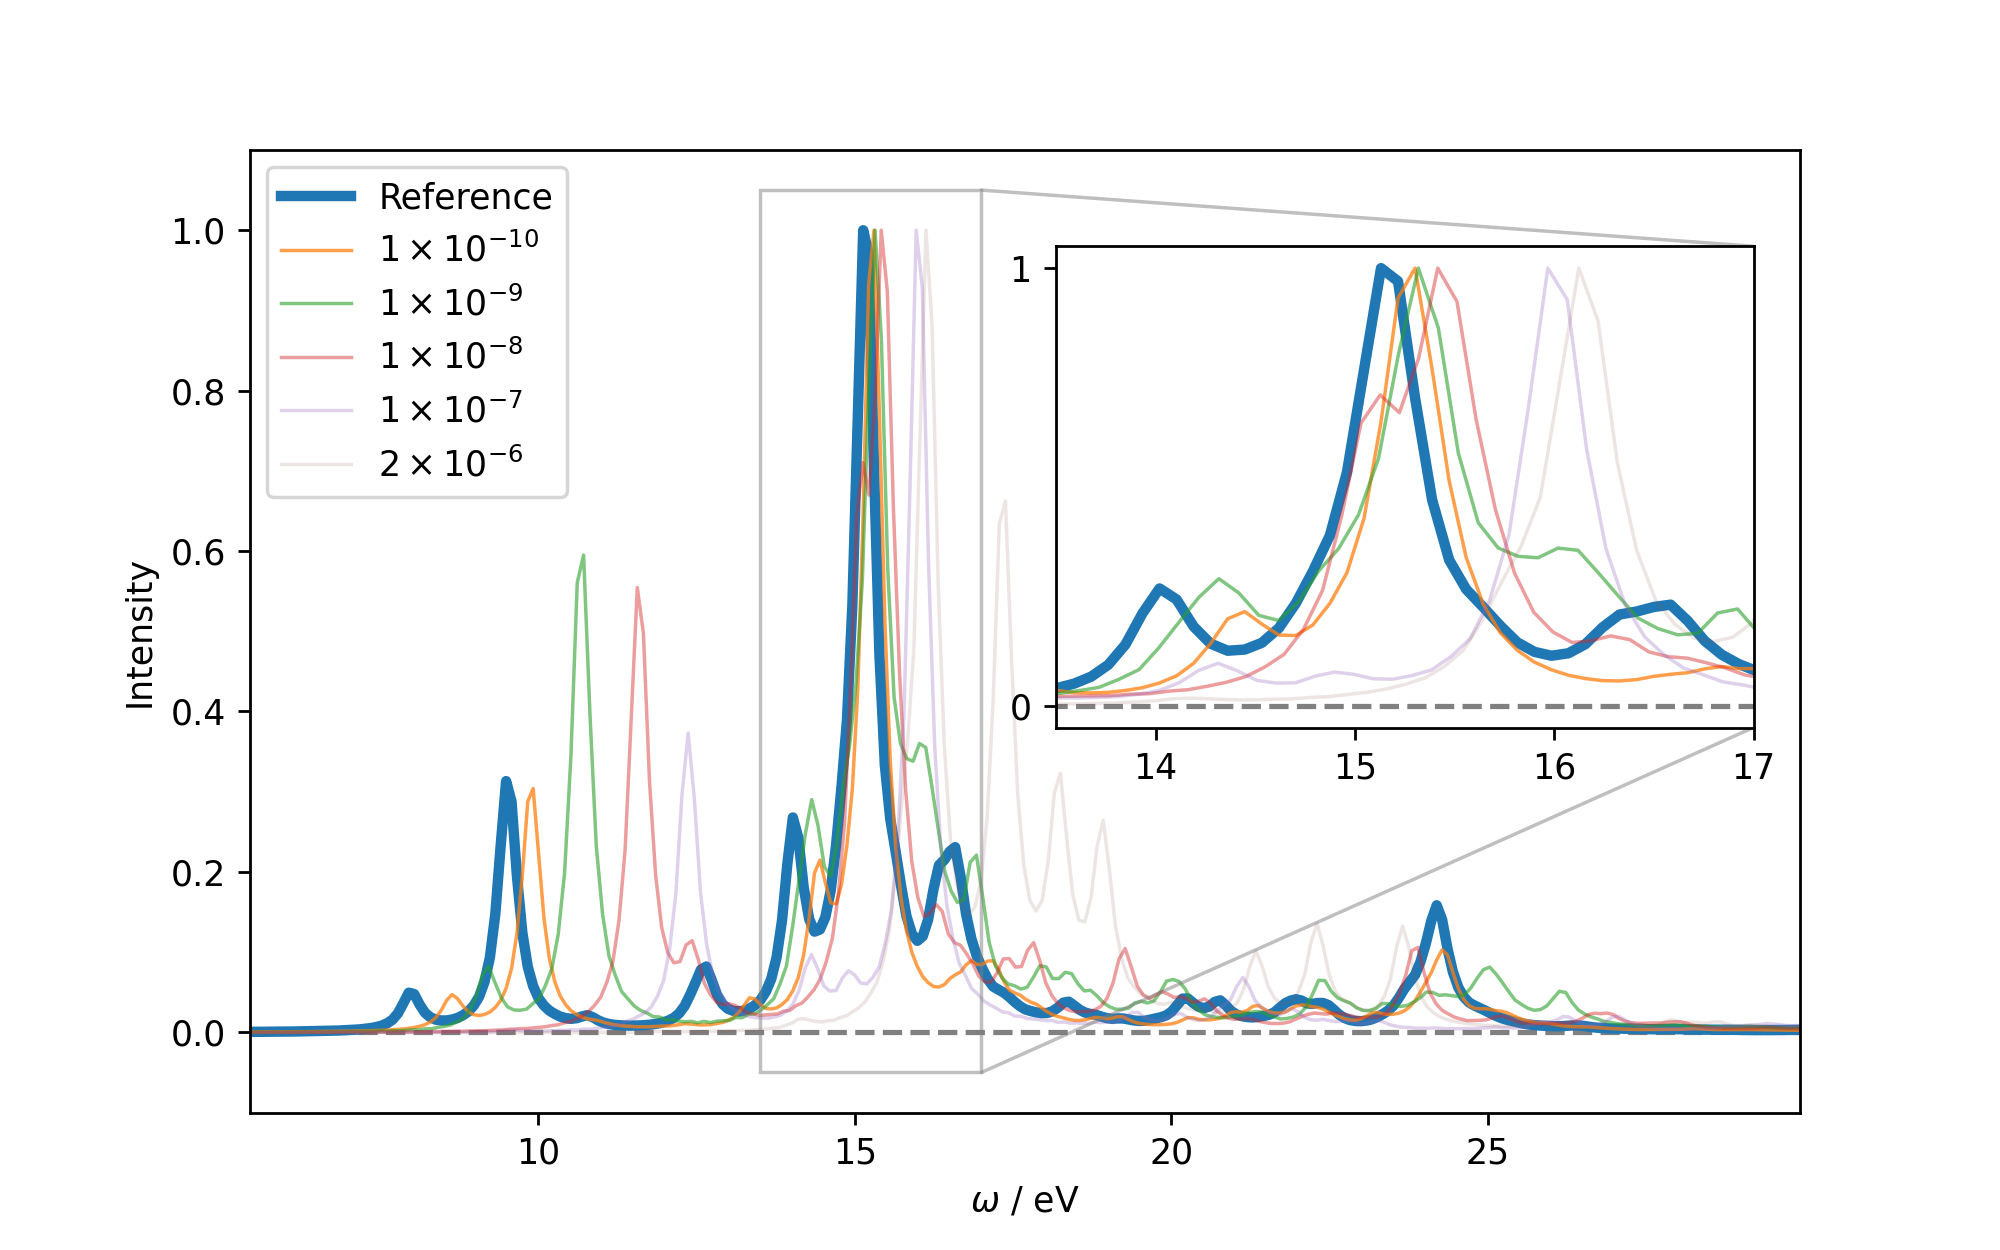
\includegraphics[scale=.6]{p3/figures/pno_abs.png}
    \caption{Reference and PNO absorption spectra for five cutoffs: 
    [$1\times 10^{-10}$, $1\times 10^{-9}$, $1\times 10^{-8}$, $1\times 10^{-7}$, 
    $2\times 10^{-6}$] corresponding to [$93\%$, $82\%$, $63\%$, $44\%$, $24\%$]
    of the MO virtual space, respectively.}
    \label{fig:pno_abs}
\end{figure}
%For all truncated PNO virtual spaces considered, the base peak appears to within 1.5 eV of the 
%reference. 
Overall, truncated PNO virtual spaces approximate the position of the base peak well,
with the smallest space predicting a base peak within 1.5 eV of the reference,
and the two largest spaces predict this peak to within 0.2 eV of the reference.
Convergence to the reference base peak occurs from the right, indicating
a lowering of excited state energies as the size of the virtual space increases. 
This trend can also be seen for the smaller peak near 10 eV. However, convergence of the shoulder 
peaks on either side of the base peak, indicated by the inset of 
Figure~\ref{fig:pno_abs}, is less predictable. Even the largest spaces considered
do not correctly predict the excitation energy, with no clear advantage to having
93\% of the virtual space as compared to just 83\% for predicting these peaks.
This trend continues into the higher-energy range of the spectrum, with the 
performance of each cutoff being nearly indistinguishable. 

Performance of the PAO space is shown in Figure~\ref{fig:pao_abs}. 
\begin{figure} 
    \centering
    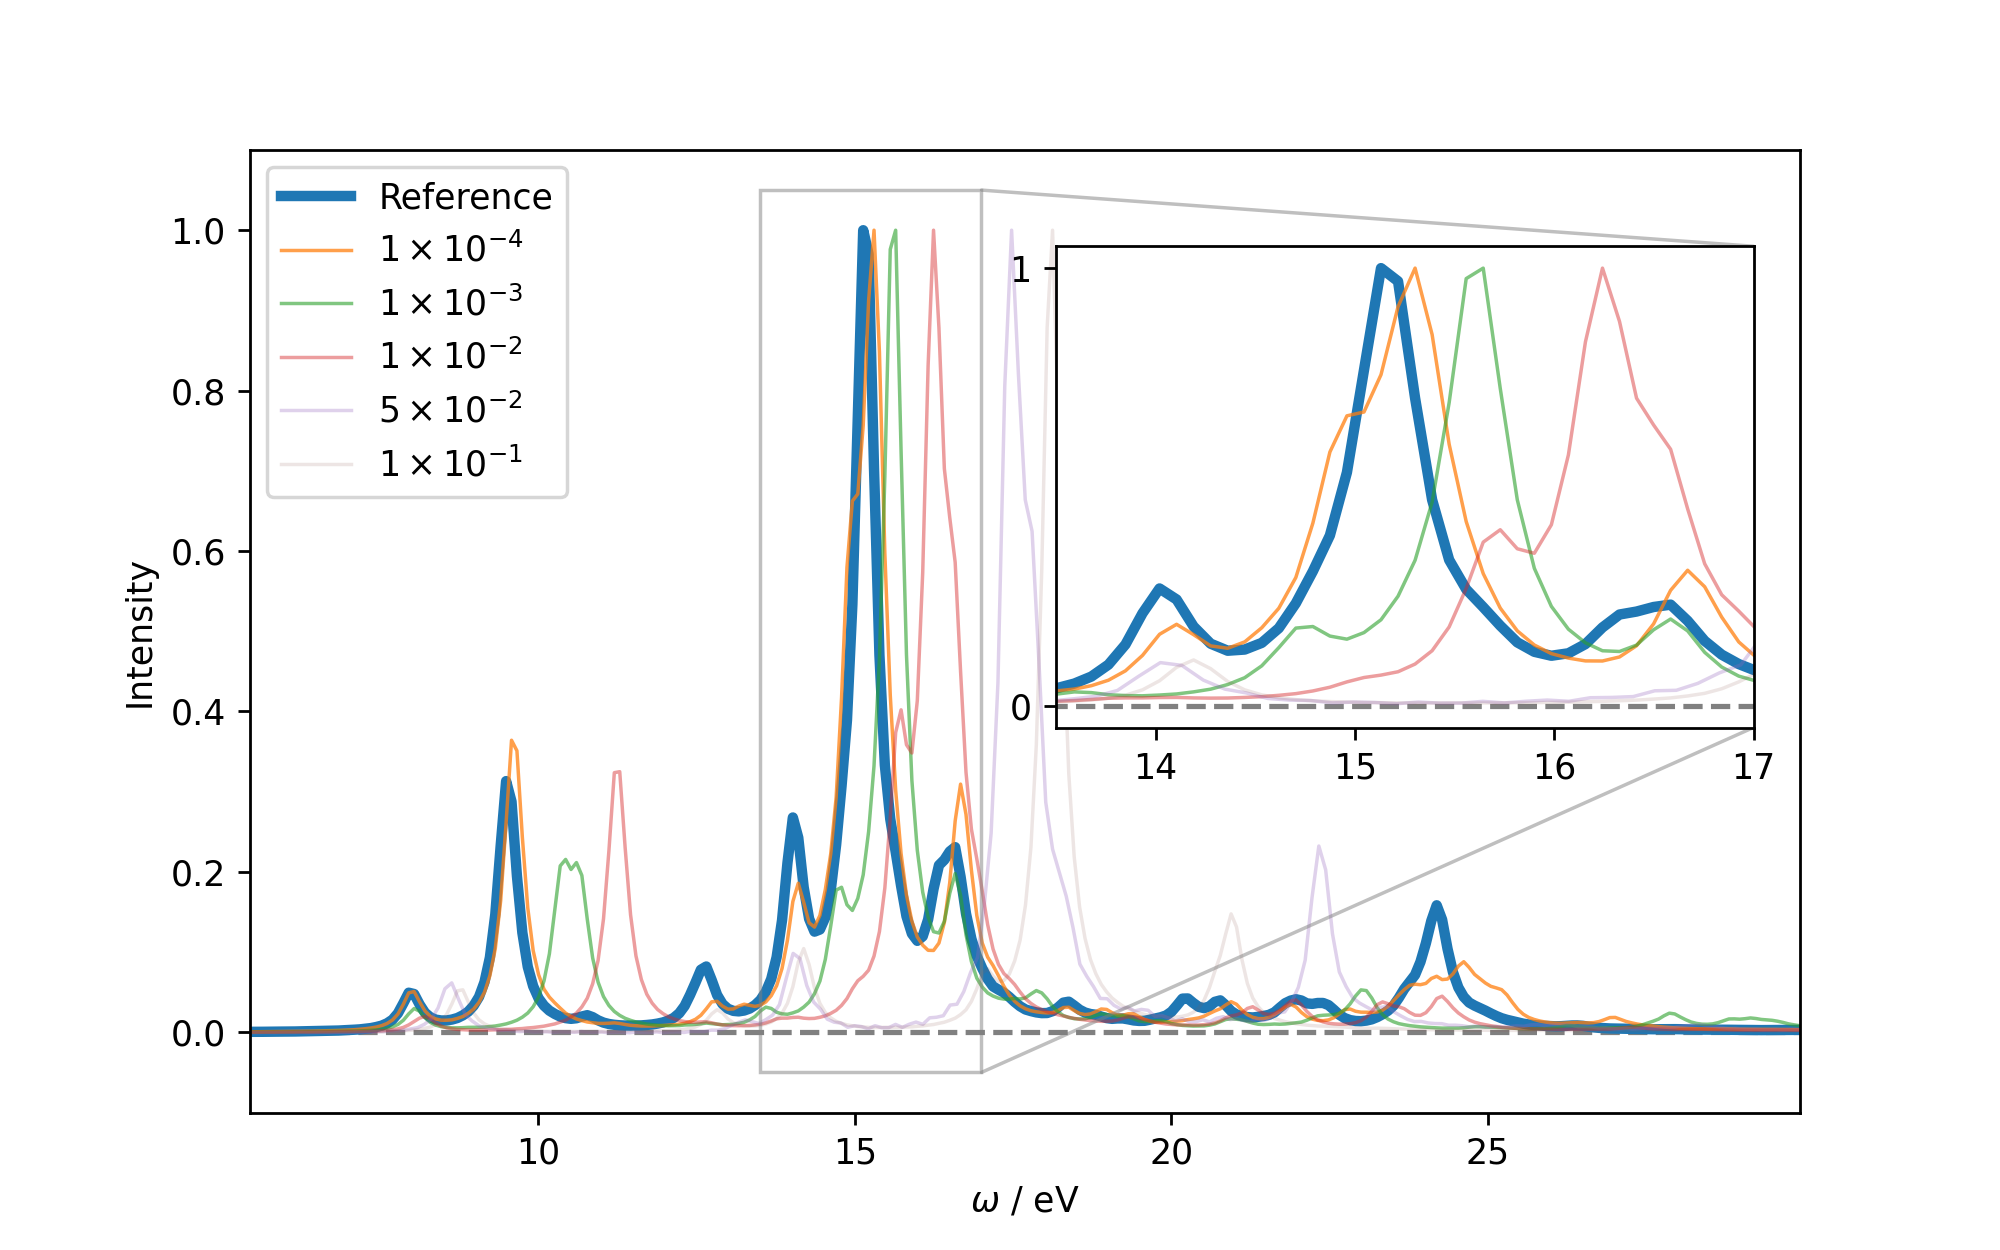
\includegraphics[scale=.6]{p3/figures/pao_abs.png}
    \caption{Reference and PAO absorption spectra for five cutoffs: 
    [$1\times 10^{-4}$, $1\times 10^{-3}$, $1\times 10^{-2}$, $5\times 10^{-2}$, 
    $1\times 10^{-6}$] corresponding to [$95\%$,$86\%$,$63\%$,$46\%$,$23\%$]
    of the MO virtual space, respectively.}
    \label{fig:pao_abs}
\end{figure}
The largest truncated PAO virtual space, on average 95\% of the MO space, accurately 
predicts the excitation energies for each major peak below 17 eV. Particularly around 10 eV, 
this is noticeably improved performance relative to the largest PNO space tested, 
with only a 2\% difference in the average size of the virtual space. 
However, accuracy rapidly declines even at 86\% of the virtual space, where the base peak
position is already worse than what was predicted with a PNO space of just 63\% of the 
MO space. Performance continues to degrade as energy increases and the average size of 
the PAO space decreases. For the final two cutoffs, at averages of 46\% and 23\% of the
MO space, the base peaks are 3 eV or more away from the reference, and no peak is 
exhibited near 25 eV. These spaces also fail to predict the second largest peak, the 
excitation just below 10 eV. 

\subsubsection{ECD} \label{sss:ecd}
Overall, neither scheme produced adequate results upon truncation of the virtual space. 
This result is not entirely surprising -- in studies of local correlation applied to 
response theory by Crawford \textit{et al}., 
\cite{McAlexander2016,Kumar2017,Crawford2019,DCunha2021} 
traditional schemes proved inaccurate for another 
electric dipole--electric dipole property, the electric polarizability.
In terms of response theory,
the polarizability (and the refractive index) is related to the \textit{real} part 
of the electric dipole--electric dipole linear response tensor 
($\boldsymbol{\alpha}_{ij}$ in Eq.~(\ref{eq:mu_exp})), 
while absorption
is related to the \textit{imaginary} part. Indeed, all linear absorptive properties
such as absorption and CD 
are related to the imaginary component of a linear response tensor, while dispersive 
properties such as refractive index and 
circular birefringence (also known as optical rotation)
are related to the real component.
\cite{Barron2004,Norman2011}
To continue, we will look at another absorptive property which is related to the mixed
electric dipole--magnetic dipole linear response tensor -- ECD.

The ECD spectrum is obtained from the Fourier transform of Eq.~(\ref{eq:ecd}).
Being a bisignate, mixed-response property, ECD is a considerable computational
challenge, similar to its dispersive counterpart circular birefringence. 
Figure~\ref{fig:pno_ecd} shows the results for an ECD spectrum in the same PNO 
orbital spaces used in the previous section.
\begin{figure} 
    \centering
    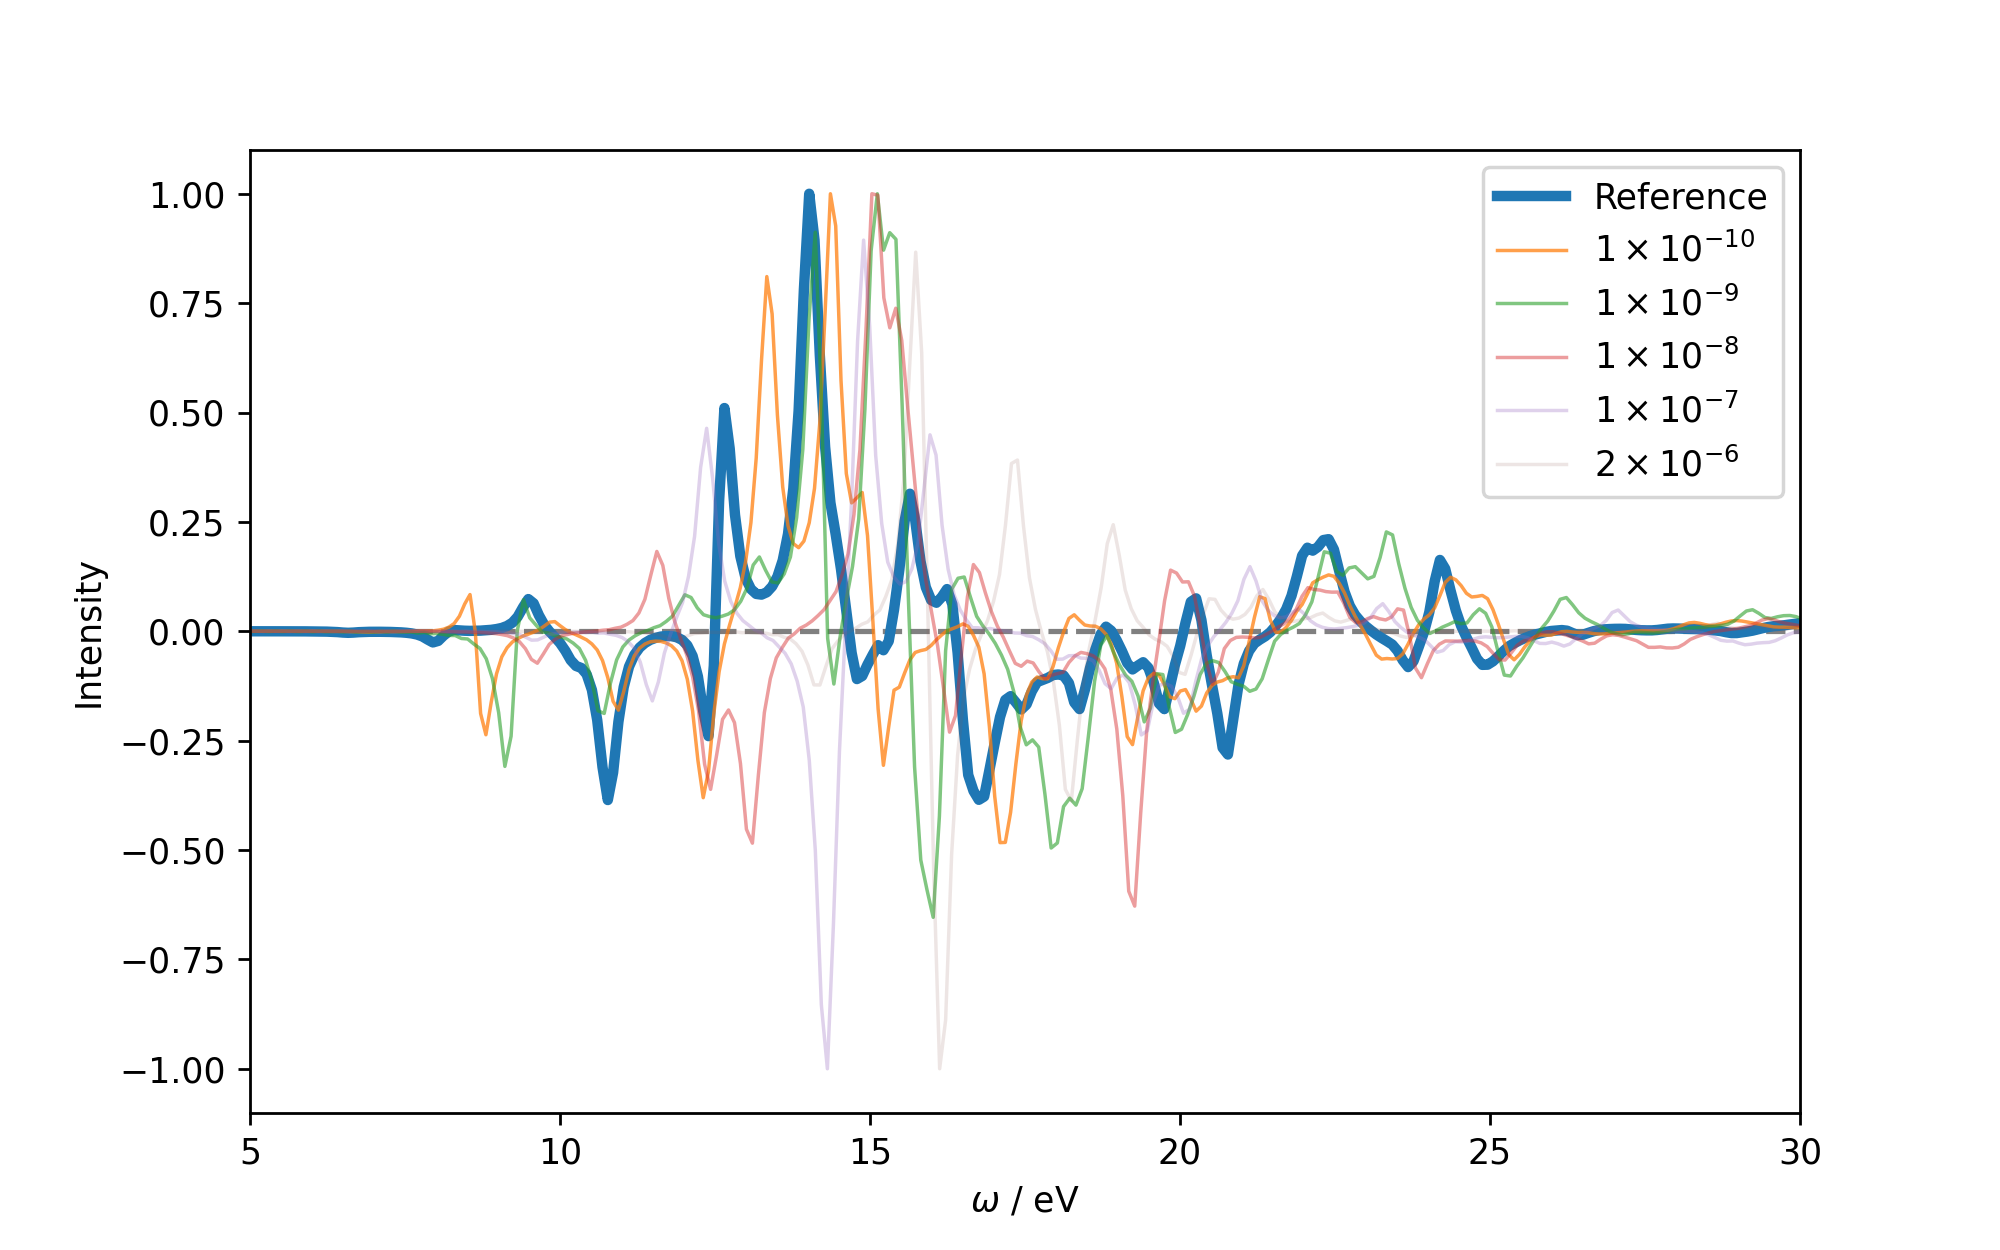
\includegraphics[scale=.6]{p3/figures/pno_ecd.png}
    \caption{Reference and PNO ECD spectra for five cutoffs: 
    [$1\times 10^{-10}$, $1\times 10^{-9}$, $1\times 10^{-8}$, $1\times 10^{-7}$, 
    $2\times 10^{-6}$] corresponding to [$93\%$,$82\%$,$63\%$,$44\%$,$24\%$]
    of the MO virtual space, respectively.}
    \label{fig:pno_ecd}
\end{figure}
The dynamic response of the magnetic dipole to the electric field in this frequency 
range is considerably more complicated than that of the electric dipole. Below 60\% of
the MO space, virtually all distinguishing characteristics of the reference 
spectrum are unidentifiable. Further, at 82\%, the base peak appears to be a pair of 
peaks, more resembling the pair of peaks appearing just above 15 eV in the 
reference spectrum, with the major peak just below 15 eV being the second strongest.
At an average of 93\%, the overall \textit{shape} of the spectrum in the 10 eV to 
20 eV range more closely resembles that of the reference; however, the excitation
energies are, in some cases, even less accurate than those of smaller PNO spaces.
The trend of lowering excited state energies with increased virtual space seen in 
Section~\ref{sss:ecd} is no longer discernible. 

As in the case of absorption, the PAO basis is not noticeably more efficient at
approximating the full MO space than the PNO space. Figure~\ref{fig:pao_ecd} 
shows the results using the same truncated PAO spaces as in Section~$\ref{sss:abs}$.
\begin{figure} 
    \centering
    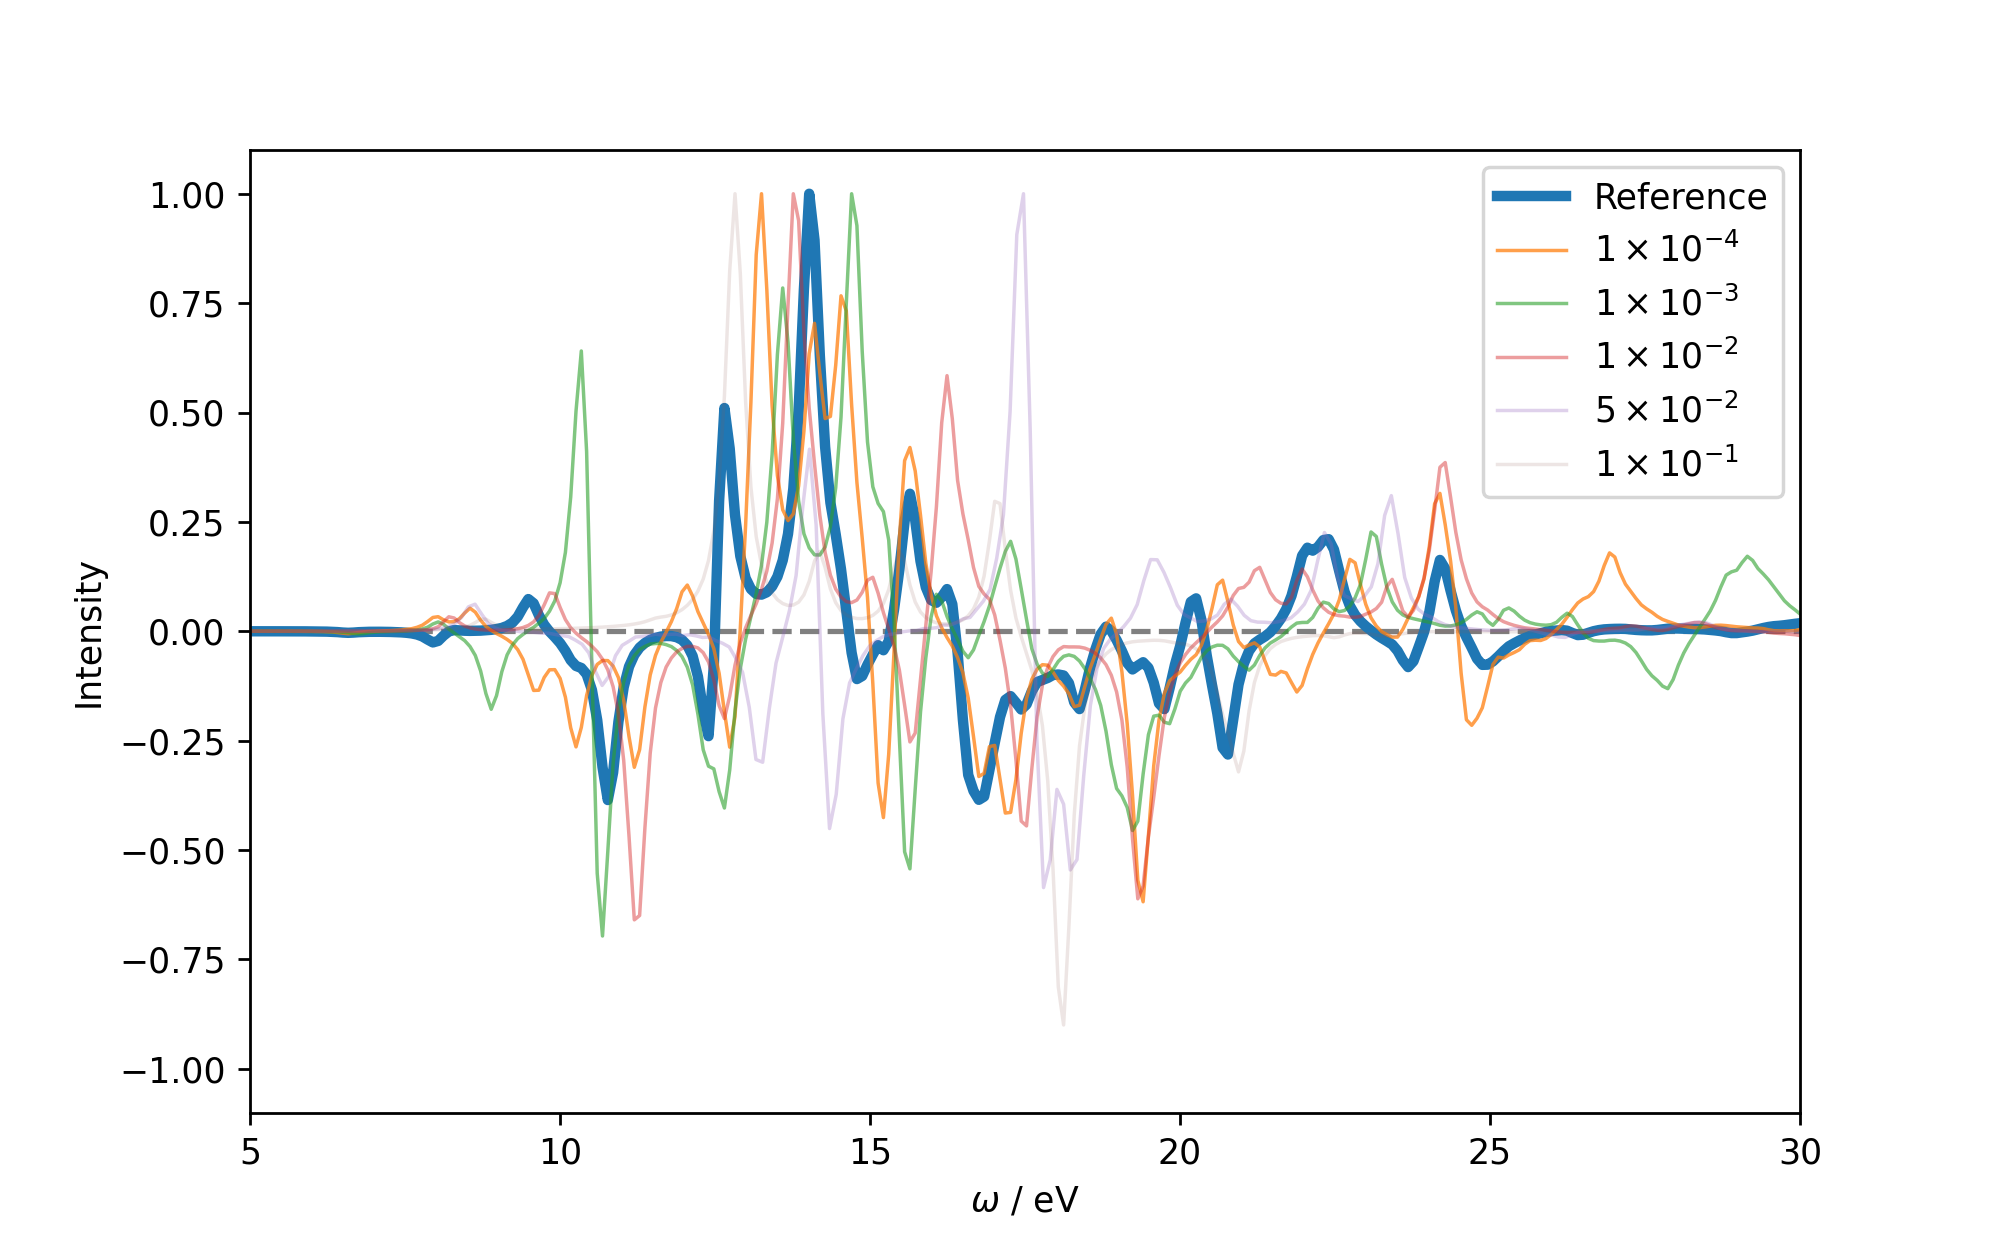
\includegraphics[scale=.6]{p3/figures/pao_ecd.png}
    \caption{Reference and PAO ECD spectra for five cutoffs: 
    [$1\times 10^{-4}$, $1\times 10^{-3}$, $1\times 10^{-2}$, $5\times 10^{-2}$, 
    $1\times 10^{-6}$] corresponding to [$95\%$,$86\%$,$63\%$,$46\%$,$23\%$]
    of the MO virtual space, respectively.}
    \label{fig:pao_ecd}
\end{figure}
The performance of the PAO basis near the base peak varies wildly with truncation,
as in the PNO case. In the low-frequency region, the PAO results are considerably 
worse -- see the two negative peaks between 10 eV and 15 eV. Curiously, the 
largest PAO spaces considered predict significant peaks above 25 eV that are not 
present in the reference, any of the PNO spaces tested, or the smaller PAO
spaces. This suggests a strong sensitivity of the response of the wave function
to the completeness threshold used for determining the occupied domains.
%fundamentally different electronic structure in the
%presence of the perturbing field, which is a direct result of the charge-based 
%completeness threshold used for determining the occupied domains.
%albeit at very large frequencies which are of little practical use.

\subsection{Amplitude Dynamics} \label{ss:amps}
As evidenced by the preceding data, the truncated PNO and PAO virtual spaces do not
efficiently model the wave function in the presence of a perturbing EMF. As noted in
Section~\ref{sss:abs}, these shortcomings are well-documented in the case of response
theory. However, a real-time formalism offers the opportunity to analyze the wave 
function in great detail over time, perhaps shedding light on \textit{where} and 
\textit{how} the locally correlated wave functions are deficient. The following
section will scrutinize the $t_\mu$ and $\lambda_\mu$ amplitudes of 
Eqs.~(\ref{eq:t_mu}) and (\ref{eq:l_mu}), respectively, in hopes of determining the 
important fluctuations in the wave function and whether these spaces sufficiently 
capture these changes.

Response to external perturbations by the CC amplitudes give rise to
dynamic energetics and properties. In the past, distributions of perturbed amplitudes
(relative to their ground-state counterparts) have been used to justify the 
difficulty in computing response functions with local correlation methods in the 
frequency domain. 
\cite{McAlexander2016,Crawford2019,DCunha2021} 
However, initial findings show that in RTCC, the relative distribution of amplitudes 
by magnitude is not significantly impacted.\cite{Crawford2019} 
Despite this, typical means of exploiting amplitude
sparsity have been shown to be inefficient by the preceding sections. 
First, to understand the response of 
the amplitudes to the external perturbation, we plot the 
change in the norm of the amplitude tensors relative to the ground-state amplitudes 
as a function of time in Figure~\ref{fig:norm}.
\begin{figure} 
    \centering
    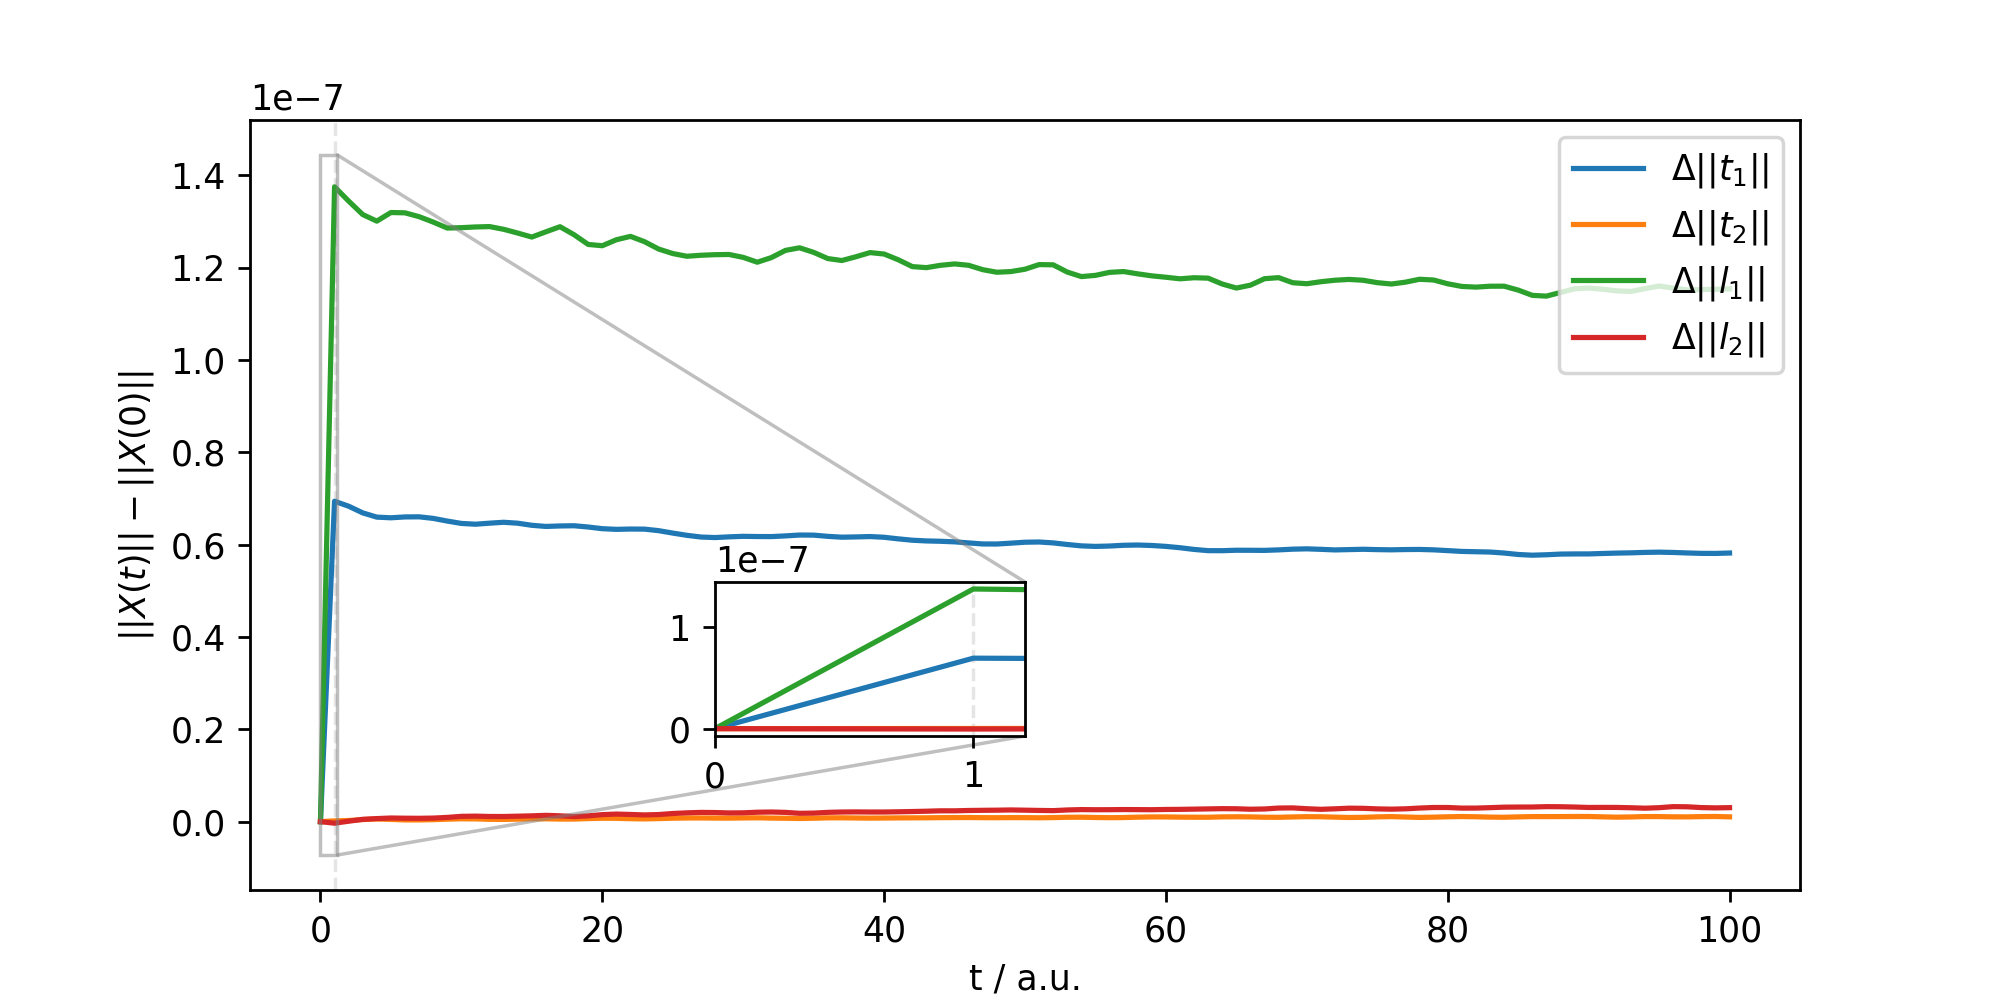
\includegraphics[scale=.6]{p3/figures/amp_norm.png}
    \caption{Time-dependent change in the norm of the amplitude 
    tensors relative to the ground-state amplitudes.
    (Field and step parameters remain unchanged, and 
    the amplitude norm is taken at every 1 a.u.)}
    \label{fig:norm}
\end{figure}
Results for the untruncated PNO and PAO spaces are identical to those
for the MO space, as the unitary transformations resulting from untruncated localized virtual spaces
in Eqs.~(\ref{eq:rotate}) preserves the tensor norm.
Amplitude norms from propagations carried out in truncated PNO and PAO spaces
are nearly indistinguishable (see SI).

Figure~\ref{fig:norm} shows that the magnitude of the response by the wave function
is predominantly within the singles amplitudes $t_1$ and $\lambda_1$. This is 
consistent with the notion that singles are paramount for the computation of 
response properties.\cite{Christiansen1995,Koch1997} However, the form of Eq.~(\ref{eq:pair_D})
does not include any contributions by singles, due to being built from MP2-level
amplitudes where singles do not contribute until at least the second order 
in the wave function and fourth order in the energy. This suggests that even in schemes
which seek to include the EMF perturbation in the construction of the reduced virtual space,
such as PNO++,\cite{DCunha2021} response of the singles should be considered.

Aside from the matrix norm, we can also inspect the individual amplitudes to track
their evolution in time. The heat maps in Figure~\ref{fig:amps} show the difference 
in $t_1$ amplitudes, relative to the ground state, for three time steps selected 
from the first 100 a.u. of the simulation.
\begin{figure}
    \begin{subfigure}{.5\textwidth}
        \centering
        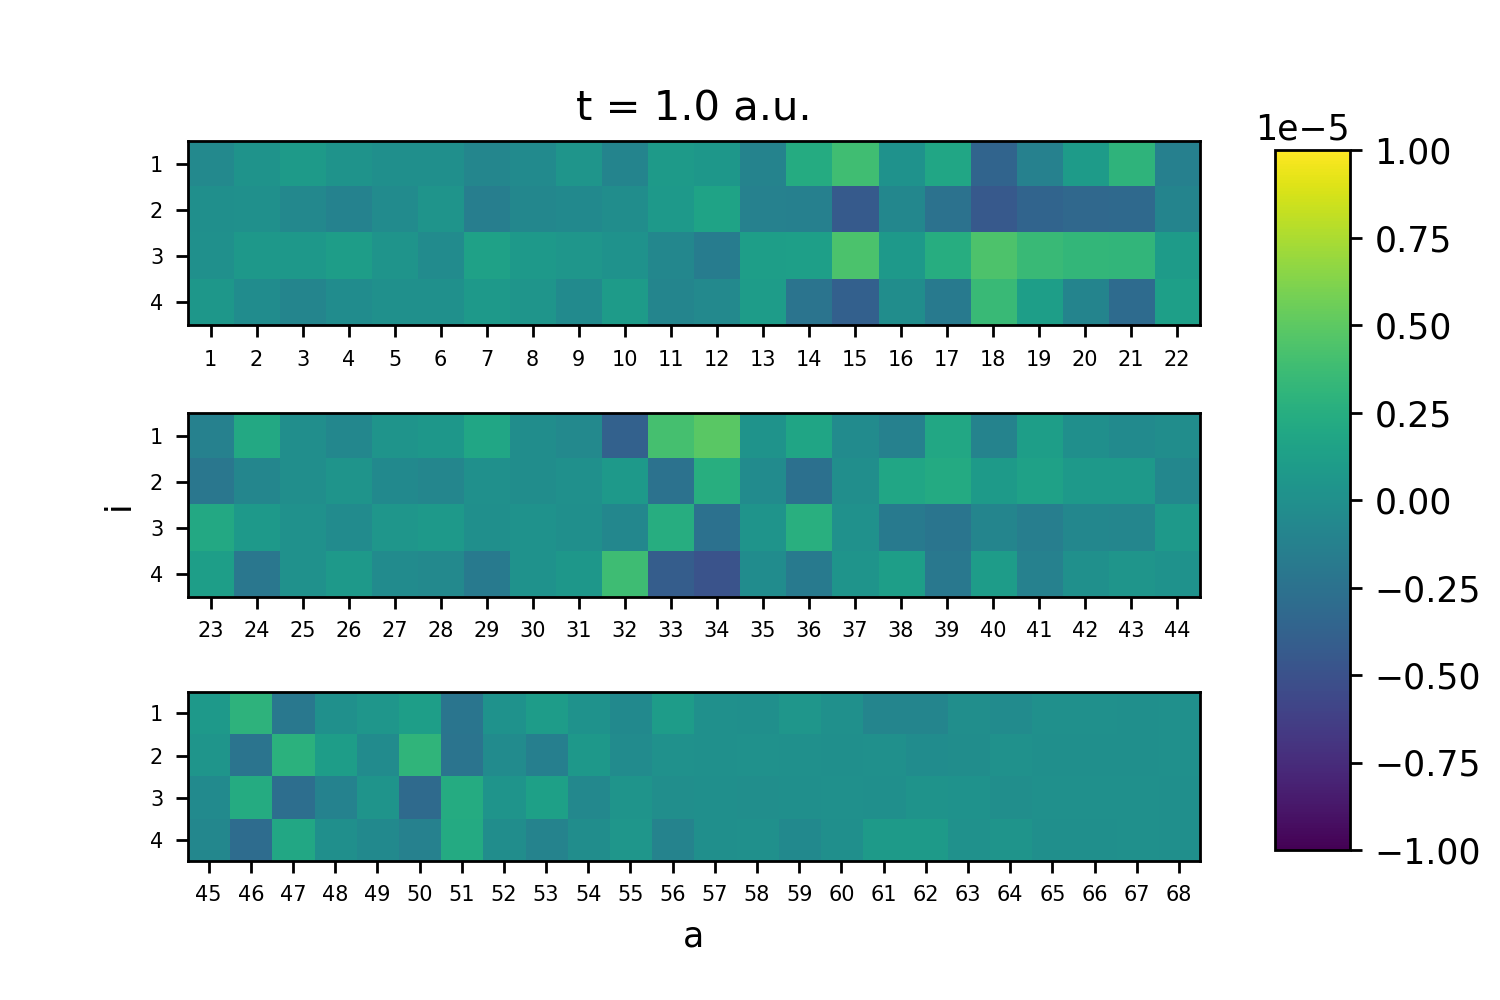
\includegraphics[scale=0.5]{p3/figures/MO_delta_t1_1.png}
        \caption{}
        \label{fig:MO_t1_1}
    \end{subfigure}%
    \begin{subfigure}{.5\textwidth}
        \centering
        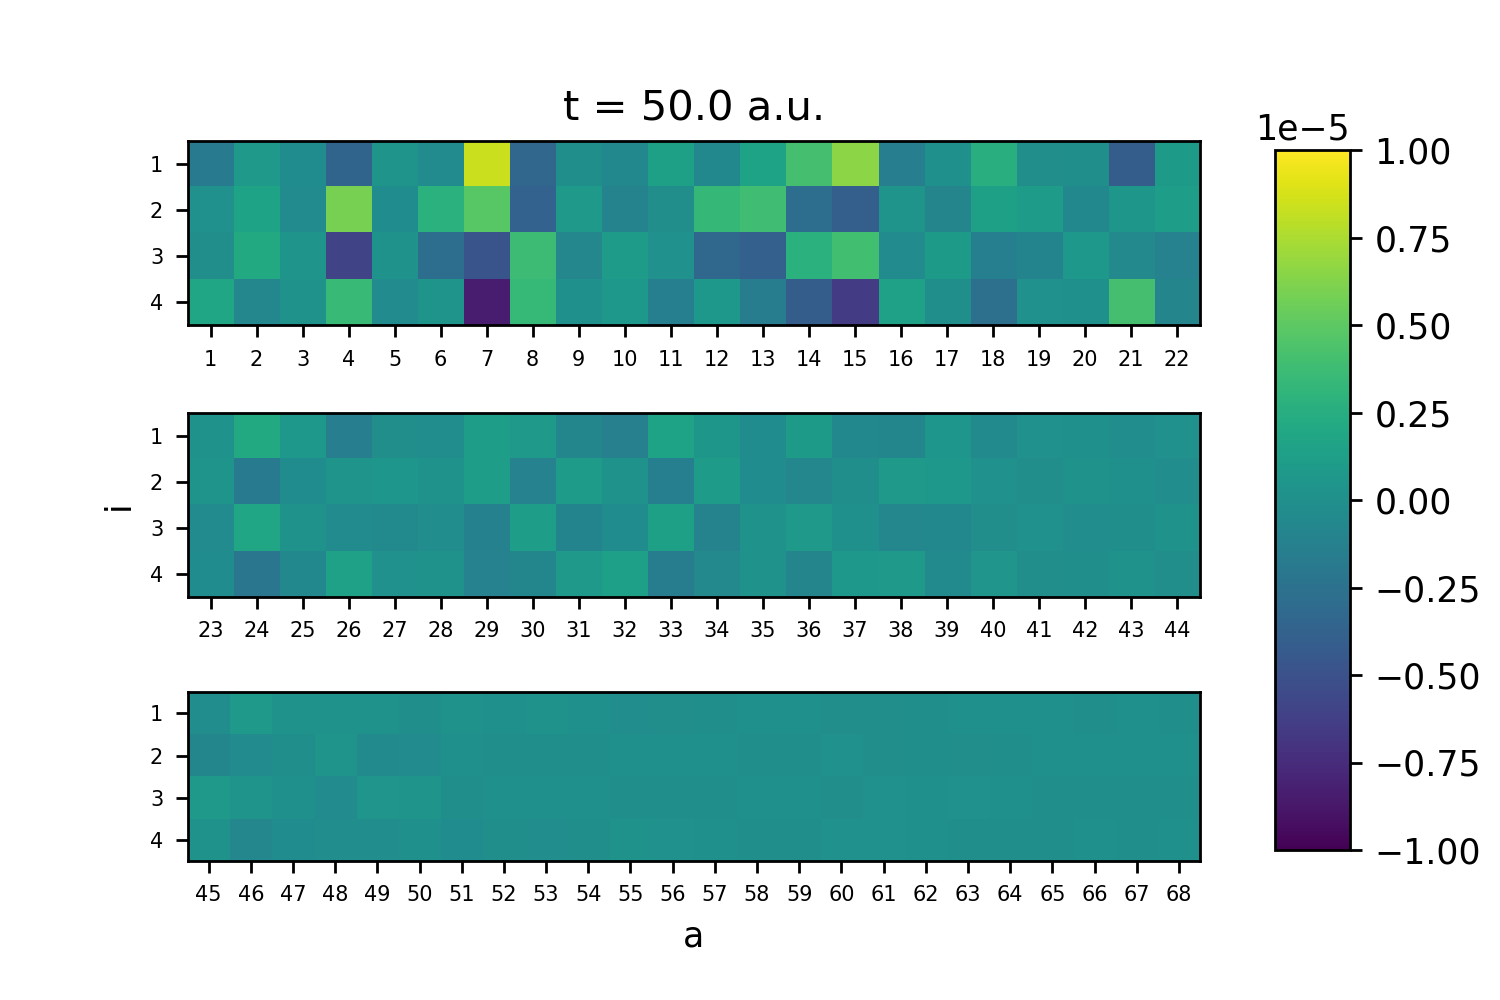
\includegraphics[scale=0.5]{p3/figures/MO_delta_t1_50.png}
        \caption{}
        \label{fig:MO_t1_50}
    \end{subfigure}
    \begin{subfigure}{.5\textwidth}
        \centering
        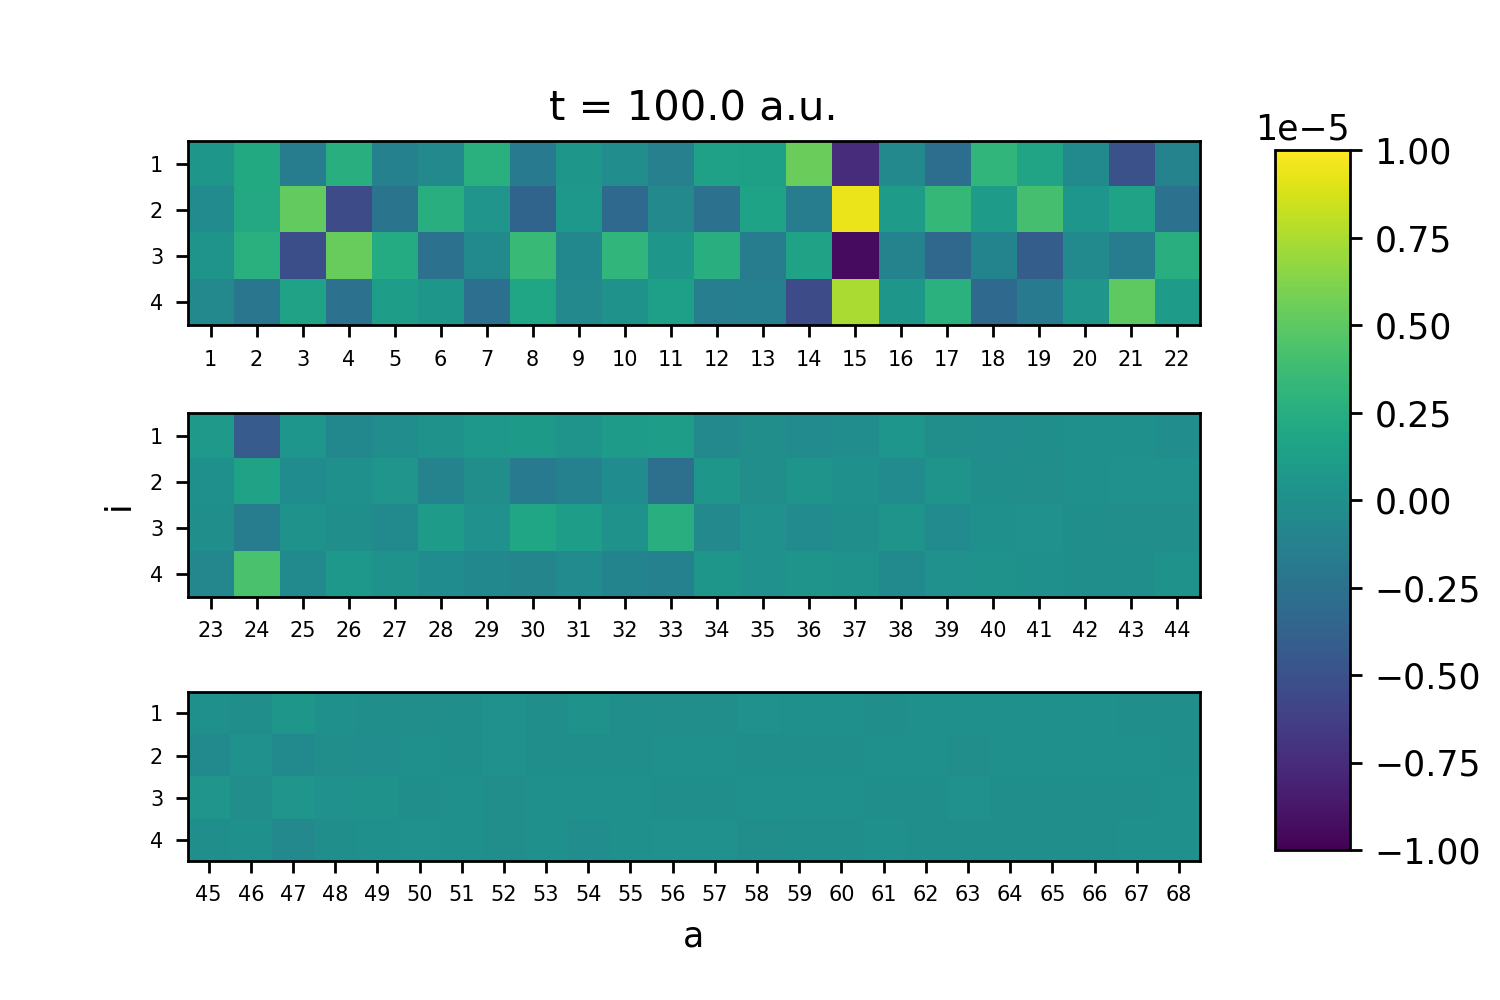
\includegraphics[scale=0.5]{p3/figures/MO_delta_t1_100.png}
        \caption{}
        \label{fig:MO_t1_100}
    \end{subfigure}
    \caption{MO-basis $t_1$ amplitude deviations from $t = 0$ after (a) 1 a.u., (b) 50 a.u., and 
    (c) 100 a.u. of time propagation. Each row contains the same four occupied orbital indices
    and a subset of virtual indices as indicated by the x-axis labels.}
    \label{fig:amps}
\end{figure}
The amplitudes are ordered by the orbital energies of the associated MOs. 
The amplitudes which experience significant oscillations vary throughout the simulation,
though there are several discernible trends. First, most large amplitude deviations
are associated with all occupied orbitals simultaneously. This is due to the relatively small size of 
the system, with only four occupied orbitals, all of which are likely important in the
description of the ground- and excited-state wave functions. Secondly, 
at any given time during the propagation,
a large number of amplitudes have not significantly deviated from their ground state values.
This supports the notion
that relative sparsity is maintained within the amplitudes throughout the simulation,
but this sparsity is distributed differently throughout the amplitude tensors as
the wave function is propagated.  

A third trend is that amplitudes which respond strongly tend to be associated with 
low-energy virtual orbitals. Chemical intuition would suggest that energetically 
low-lying molecular orbitals will be the most involved in electronic excitations.
However, while amplitude responses are indeed larger for lower-energy virtual orbitals, 
smaller amplitude 
deviations in Figure~\ref{fig:amps} extend far into the virtual space. This explains
the difficulty of simply truncating with respect to orbital energy: the 
high-energy MOs are still important to the time-evolution of the wave function 
in the presence of an EMF. 

Figure~\ref{fig:pno_amps} shows the $t_1$ amplitudes for the same simulation,
rotated into the untruncated PNO basis using $Q_{ii}$ as defined in
Eq.~(\ref{eq:Q_pno}).
\begin{figure}
    \begin{subfigure}{.5\textwidth}
        \centering
        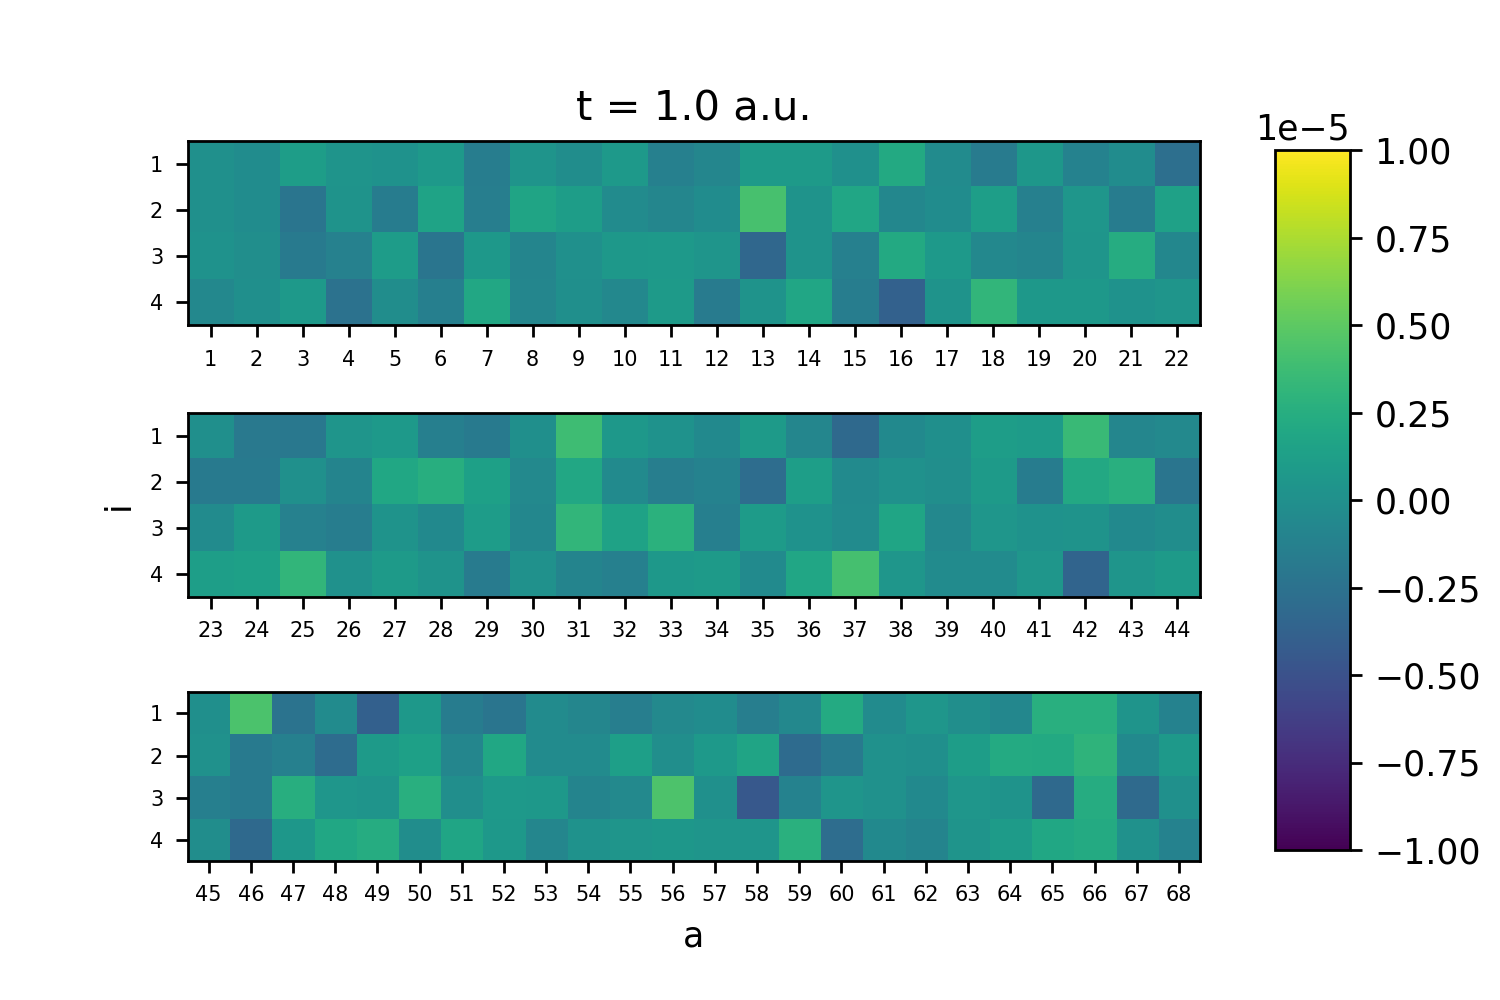
\includegraphics[scale=0.5]{p3/figures/PNO_delta_t1_1.png}
        \caption{}
        \label{fig:PNO_t1_1}
    \end{subfigure}%
    \begin{subfigure}{.5\textwidth}
        \centering
        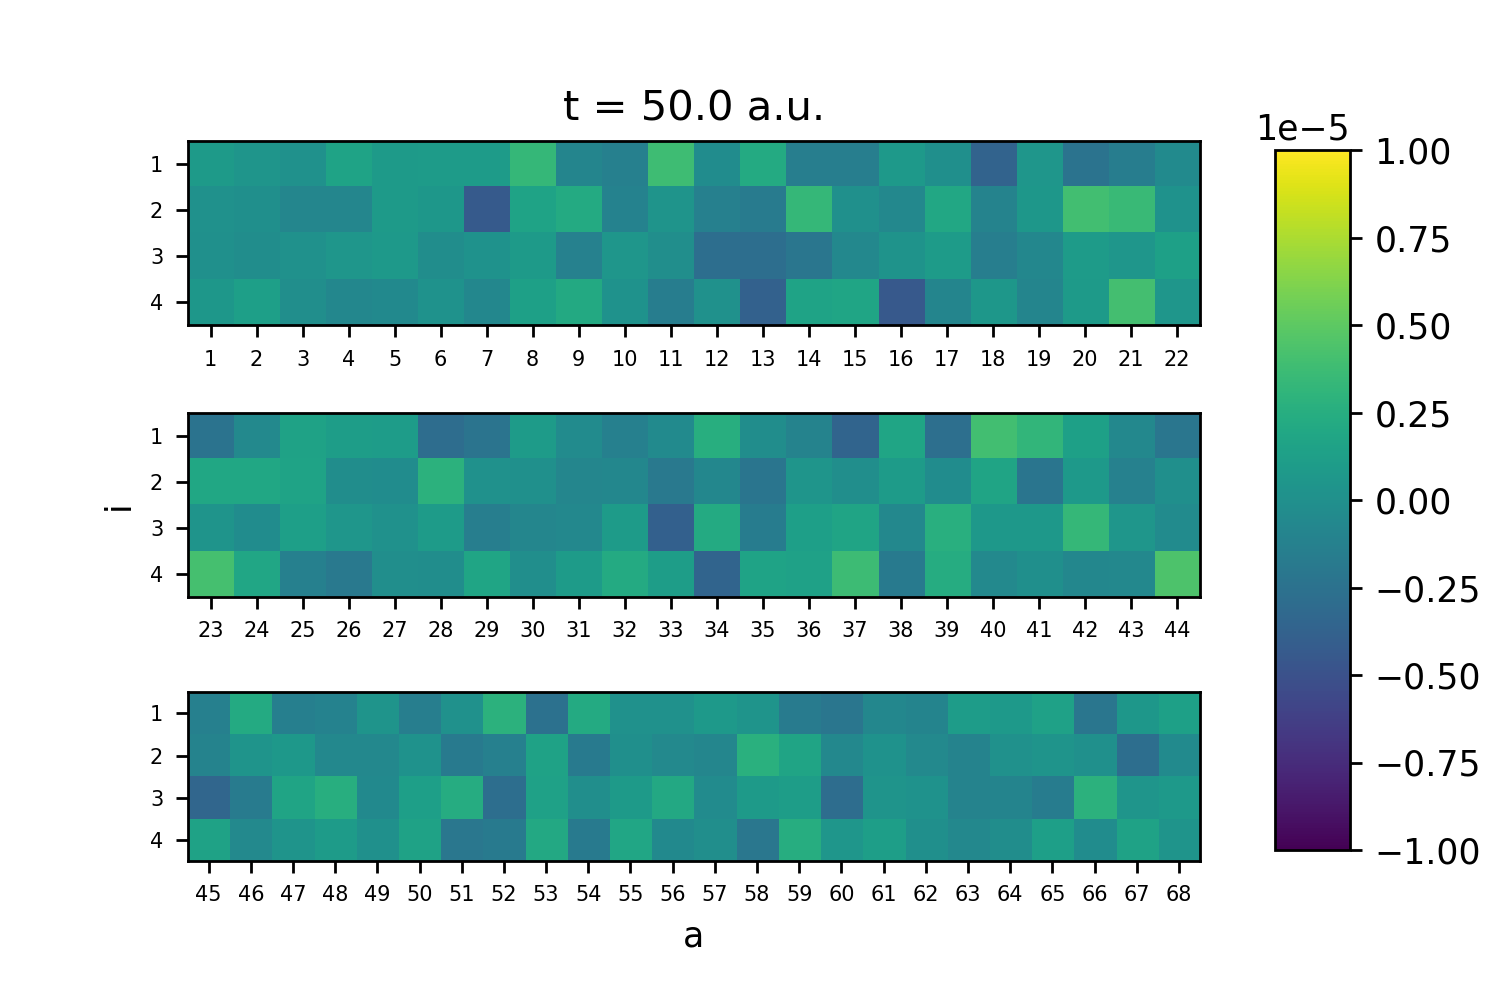
\includegraphics[scale=0.5]{p3/figures/PNO_delta_t1_50.png}
        \caption{}
        \label{fig:PNO_t1_50}
    \end{subfigure}
    \begin{subfigure}{.5\textwidth}
        \centering
        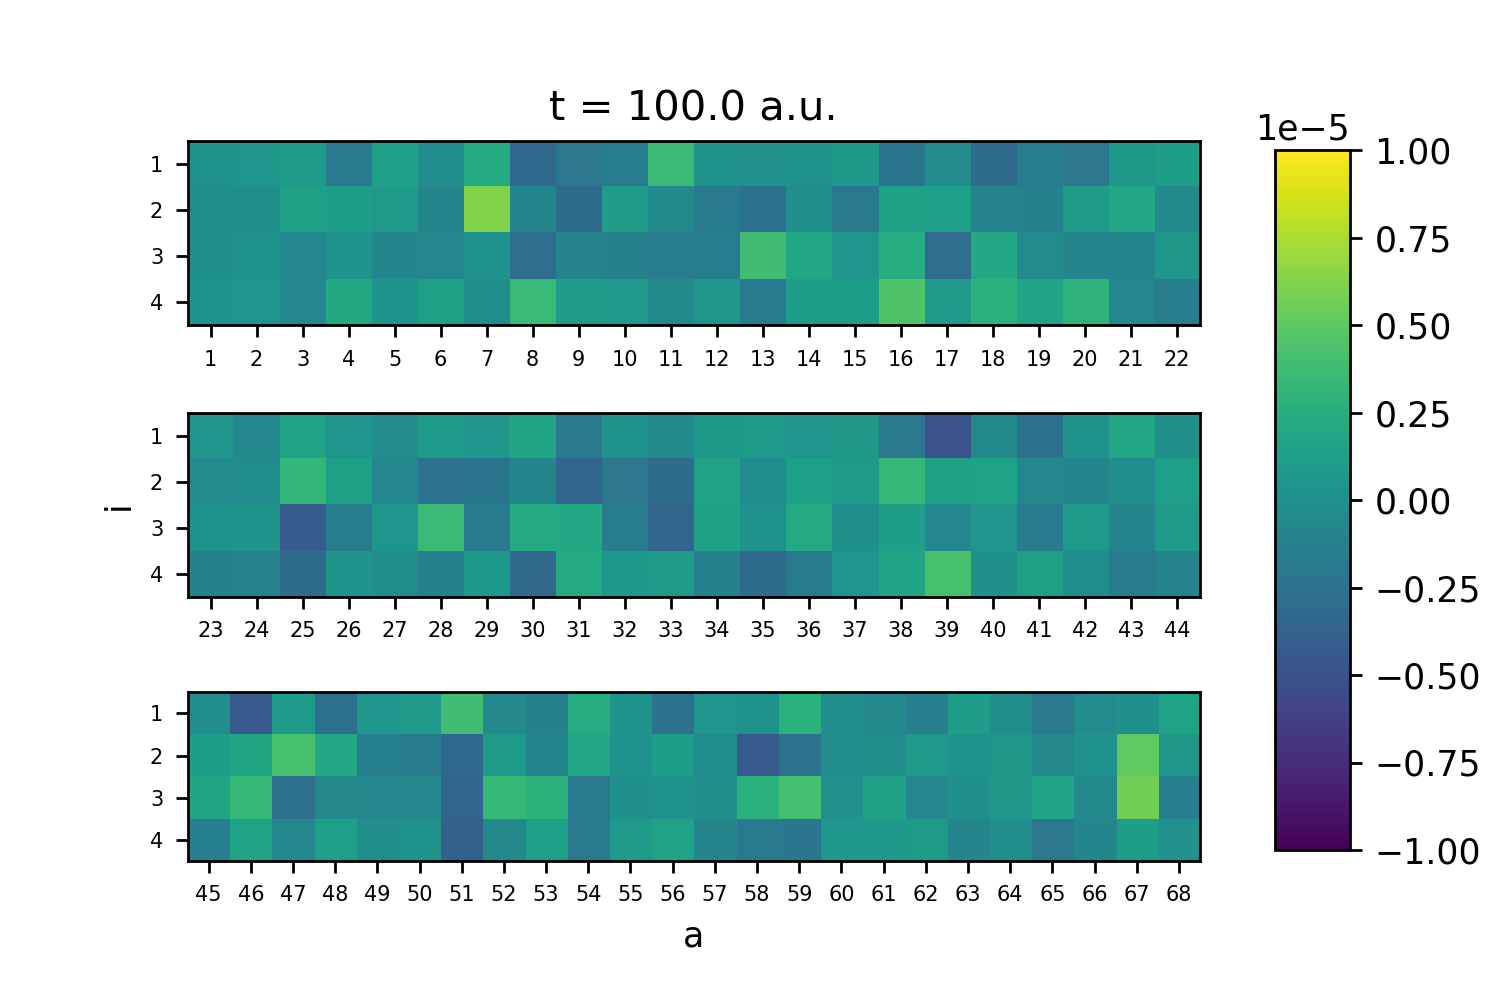
\includegraphics[scale=0.5]{p3/figures/PNO_delta_t1_100.png}
        \caption{}
        \label{fig:PNO_t1_100}
    \end{subfigure}
    \caption{PNO-basis $t_1$ amplitude deviations from $t = 0$ after (a) 1 a.u., (b) 50 a.u., and 
    (c) 100 a.u. of time propagation. Each row contains the same four occupied orbital indices
    and a subset of virtual indices as indicated by the x-axis labels.}
    \label{fig:pno_amps}
\end{figure}
(It should be noted that, due to redundancy in the AO-based virtual 
spaces for each pair, PAO-basis amplitudes cannot be compared directly in 
this manner.)
It can be immediately seen that the amplitude deviations
are less sparse in the PNO basis after the application of the EMF. 
Many more amplitudes exhibit
perceivable differences, and strong deviations (magnitudes approaching 
$1\times 10^{-5}$) are no longer present. This is a clear demonstration
of the issue with truncating orbital spaces based on the present criterion ---
rather than exploiting sparsity, the amplitude tensors have become less sparse.
It may also suggest a recipe for building a more appropriate 
virtual space for truncation. 
In the following section, we propose some alternative schemes based on the 
literature and the results of this study.
%In the following section, we compare a selection
%of orbitals which correspond to strong amplitude deviations in the MO basis 
%(specifically virtuals 3, 4, 7, and 15)
%based on orbital spatial extent to determine if this may be a possible criterion 
%for truncation of the virtual space.

\subsection{Possible Alternatives} \label{ss:alt}
\begin{figure}
    \centering
    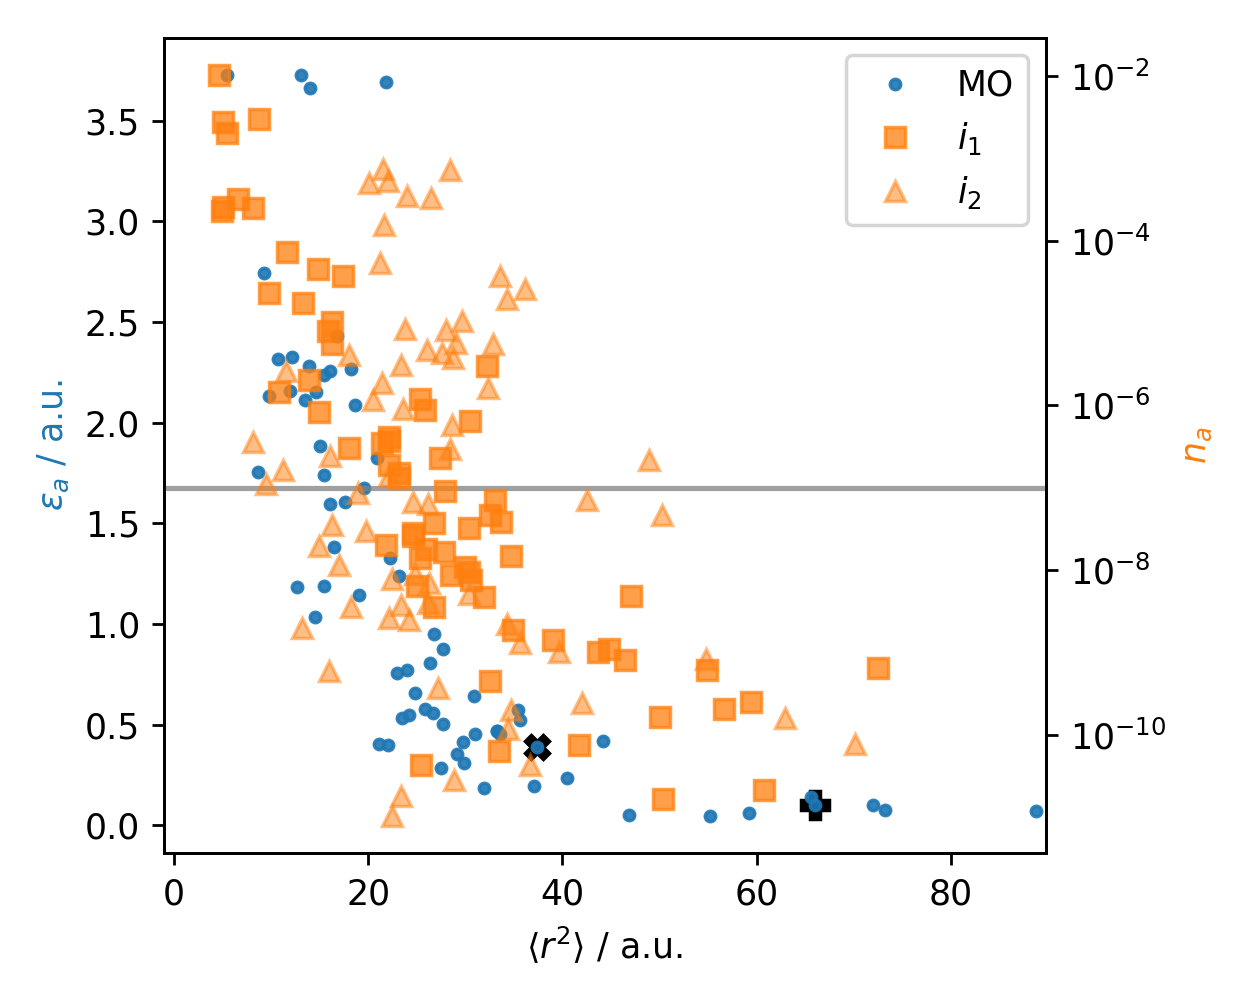
\includegraphics[scale=0.75]{p3/figures/extent.png}
    \caption{Virtual MO energy $\epsilon_a$ and the
    occupation number $n_a$ (plotted on a log scale)
    for unique PNO spaces $i_1$ and $i_2$ 
    versus orbital extent in arbitrary units.
    Virtual MOs 7 and 15 are denoted by a solid $\boldsymbol{+}$ 
    and $\boldsymbol{\times}$, respectively.
    The horizontal line denotes a PNO cutoff 
    of $1\times 10^{-7}$.}
    \label{fig:extent}
\end{figure}
Figure~\ref{fig:extent} shows the virtual MO energy $\epsilon_a$ and the 
PNO occupation number $n_a$ plotted against the orbital extent
$\langle r^2 \rangle$ in arbitrary units. 
In the PNO basis, a unique virtual space is prepared
for every occupied pair, resulting in 16 unique spaces for the four occupied
spatial orbitals $i$. However, for transforming
a single orbital index, we only require the diagonal rotation matrices,
\textit{i.e.}, $Q_{ii}$. There are four such spaces; however, by symmetry,
only two are unique. Both are included in Figure~\ref{fig:extent}. 

Truncation of the PNO space begins from the bottom of Figure~\ref{fig:extent}. 
At an occupation number cutoff of $1\times 10^{-7}$ (indicated by a horizontal
line), all orbitals below this line are neglected in the PNO space. Roughly
66\% of the virtual space lies in this region. From these data, it is clear
that even modest truncation of the virtual space neglects the diffuse 
regions of the wave function, which are important for excited-state
properties in systems with significantly delocalized characteristics,
such as systems containing Rydberg-type excitations.

%Table~\ref{ta:ext} reports the orbital extent $\langle r\rangle$ for virtual orbitals $a$
%corresponding to four of the strongest deviations in Figure~\ref{fig:amps}. 
%These orbitals are labeled 4, 7, 8, and 15, in
%both the MO and PNO basis. In the PNO basis, a unique virtual space is prepared
%for every occupied pair, resulting in 16 unique spaces for the four occupied
%spatial orbitals $i$. However, for transforming
%a single orbital index, we only require the diagonal rotation matrices,
%\textit{i.e.}, $Q_{ii}$. There are four such spaces; however, by symmetry, the domains of occupied
%orbitals 1 and 4 are the same, as are 2 and 3. Thus, orbital extents for only those
%two unique orbital spaces $i_1$ and $i_2$  are shown.
%\begin{table}
%    \centering
%    \begin{tabular}{|c|c|c|c|}
%        \hline
%%        $a$ &   MO  &   PNO   &        \\  
%        $a$ &  MO  &   \multicolumn{2}{c|}{PNO} \\  
%        \hline
%%        \multicolumn{2}{|c|}{}  & $i_1$   & $i_2$  \\ 
%            &       & $i_1$   & $i_2$  \\
%        \hline
%%         3  & 59.23 & 7.9     & -24.67 \\ 
%%        \hline
%         4  & 88.76 & -13.08  & -3.13  \\ 
%        \hline
%         7  & 66.00 & 0.73    & -0.07  \\ 
%        \hline
%         8  & 65.56 & -3.91   & -10.35 \\ 
%        \hline
%         15 & 37.39 & -15.11  &  1.32  \\
%        \hline
%    \end{tabular}
%    \caption{Orbital spatial extent of four selected virtual orbitals in the MO
%    and PNO spaces.}
%    \label{ta:ext}
%\end{table}
%A full table of virtual orbital extents can be found in the SI. 
%In the MO basis, the orbitals in Table~\ref{ta:ext} 
%correspond to the strongest amplitude deviations in Figure~\ref{fig:amps}.
%These are also some of the most diffuse orbitals in this basis,
%far larger than the average orbital extent of 26.62.
%As expected, the spatial extent of the PNOs built upon the MOs
%are much more localized. This shows that, in the MO basis,
%strong deviations are predominantly exhibited by amplitudes 
%corresponding to virtual orbitals with a larger spatial extent,
%creating sparsity. In the PNO basis, however, the deviations 
%are evenly spread across a large number of amplitudes corresponding
%to orbitals with relatively small spatial extent, resulting in 
%less sparsity in the amplitude tensor. 
%These findings suggest that virtual domains built for excited state
%properties should seek to include orbitals with large spatial extent,
%and any truncation criterion should preserve these orbitals.

Spatial extent alone may not be a suitable criterion for truncation -- 
this would have obvious a negative impact on the accuracy of the 
correlation energy, which is inherently local in nature. 
Additionally, Figure~\ref{fig:extent} highlights virtual MOs 7 
($\boldsymbol{+}$) and 15 ($\boldsymbol{\times}$),
which correspond to the strongest deviations in 
Figures~\ref{fig:MO_t1_50} and \ref{fig:MO_t1_100}, respectively.
That these orbitals are of varying extent
demonstrates that both diffuse and contracted orbitals play a role in 
the wave function dynamics.
In order to attain a balanced description of wave function components 
important for both energy and property calculations, the combination 
of appropriately determined spaces such as the combined PNO++ approach
has been fruitful. Still neglected in this approach
are the singles amplitudes, which are absent in the MP2 wave functions
used to approximate the occupied pair domains. Schemes to include 
these effects, such as approximate CC2-level $t_1$ guess amplitudes,
may further improve the space and allow greater flexibility for 
truncation. The prospect of utilizing these 
methodologies within the current framework is promising, and work is 
underway to explore their efficiency.

%conc.tex

\section{Conclusions} \label{conc} Here we present the first application
of local correlation to RTCC simulations. The popular PNO and PAO virtual
space localization schemes are applied to the calculation of dynamic electric
and magnetic dipole moments in the presence of an explicit electric field,
providing absorption and ECD spectra, respectively. 
For a helical H$_2$ tetramer, truncation of the
localized virtual space to successively larger fractions of the canonical
virtual space resulted in convergence to the canonical result; however, this
convergence is slow, and errors in excitation energies and intensity are
present even in some of the largest spaces tested, especially for ECD. This
corroborates the results of recent studies applying locally correlated
methods to the prediction of dynamic properties in the frequency domain
using response theory.

%As in the frequency domain, there are a number of possible approaches
%to building a more appropriate virtual space which preserves accuracy in
%response properties upon aggressive truncation. 
Examining the amplitude
dynamics during the propagation, it is shown that the $t_1$ and $\lambda_1$
amplitudes respond most strongly to the field -- a large increase in the
norm of these matrices is observed upon application of the field, followed
by a steady oscillation. The $t_2$ and $\lambda_2$ tensors, by comparison,
remain relatively static throughout. 
These oscillations are largely, but not completely, localized to a selection 
of only a few orbitals, as evidenced by consideration of 
time-dependent deviations in the $t_1$ amplitudes from the ground-state.
In the localized virtual spaces tested,
these oscillations are delocalized throughout the $t_1$ and $\lambda_1$
matrices. 

Orbital extent alone cannot explain the shortcomings of 
the PNO space; however, its effect is significant. 
These results provide an insight into the importance of 
singly-substituted determinants in the time-dependent wave function in the 
presence of an electric field, as well as a potential metric to gauge the 
performance of new localization schemes for frequency- or time-domain 
calculations of dynamic response properties.
In order to attain a balanced description of wave function components 
important for both energy and property calculations, the combination 
of appropriately determined spaces such as the combined PNO++ approach
has been fruitful.\cite{DCunha2021} 
Still neglected in this approach
are the singles amplitudes, which are absent in the MP2 wave functions
used to approximate the occupied pair domains. Schemes to include 
these effects, such as approximate CC2-level $t_1$ guess amplitudes,
may further improve the space and allow greater flexibility for 
truncation. The prospect of utilizing these 
methodologies within the current framework is promising, and work is 
underway to explore their efficiency.


    \chapter{Machine-Learning Coupled Cluster Properties through a Density Tensor Representation} \label{ch:p2}
% Introduction

\section{Introduction} \label{se:intro} Dynamic molecular properties induced
by the absorption, scattering, or refraction of an electromagnetic field
(EMF) give rise to a number of experimental techniques for the detailed
investigation and characterization of molecular light-matter interactions
and structure.\cite{Barron2004} Among these properties are absorbance,
circular dichroism (CD), birefringence, Raman scattering, and many more.
These techniques are essential for modern synthetic chemistry in both
research and industrial settings.

Theoretical chemistry has become a ``full partner with experiment''
\cite{Goddard1985} in this regard, providing high-quality benchmark
calculations for affirming or even predicting many molecular properties,
saving time, and increasing certainty in spectral assignments and
molecular structure determination. Computing dynamic properties with
current \textit{ab initio} methods generally involves frequency-domain
perturbation theory, referred to as response theory, to directly calculate
the quantity of interest. \cite{Crawford2006,Norman2011,Helgaker2012}
Coupled cluster (CC) response theory\cite{Koch1990,Pedersen1997} has
emerged as a robust solution to frequency-domain property calculations,
when its cost is not prohibitive.\cite{Crawford2018,Crawford2019} Many
techniques for circumventing the high-degree polynomial scaling of
coupled cluster methods exist, with extensions of these to property
calculations and response theory providing promising results.
\cite{McAlexander2016,Kumar2017,Howard2018,DCunha2021}

However, there are several drawbacks to the response
formalism.\cite{Langhoff,Goings2018,Li2020} First and foremost, the
perturbations must be ``small'' relative to the intramolecular forces
present in the system. This immediately precludes the possibility of
simulating high-energy experiments such as X-ray spectroscopy, which
have numerous applications in materials science and beyond. Second,
only broadband excitations can be modeled straightforwardly: response
theory typically assumes a single, uniform ``kick'' perturbation
across all frequencies. Experimental apparatus, on the other hand,
can make use of complex, multi-phase procedures involving tuned laser
pulses, pump-probe analysis, \textit{etc}.\cite{Maiuri2020} Finally,
temporally controlled multi-photon events such as high harmonic generation
(HHG)\cite{Lewenstein1994,Gorlach} lie outside the realm of the response
formalism. Together, these drawbacks mean a wide variety of experiments
cannot be predicted or supplemented with response theory calculations. To
overcome this, we must move to non-perturbative, time-domain electronic
structure theory, \cite{Goings2018,Crawford2019,Li2020} where there are
fewer limitations on the form of the perturbing EMF.

The alternative of real-time CC (RTCC) methods has been discussed
nearly as far back as the origins of CC itself in the realm of nuclear
physics.\cite{Hoodbhoy1978,Hoodbhoy1979,Gunnarsson78} More recently, a
renewed interest in real-time coupled cluster has developed for the reasons
discussed above. In the past 10 years, several implementations have been
reported, \cite{Huber2011,Kvaal2012,Nascimento2019,Pedersen2019,Park2019}
with new insights into the aspects of numerical
integration\cite{Pedersen2019,Kristiansen2020} and
interpretation\cite{Pedersen2019,Pedersen2021} as
well as applications for a number of spectral properties.
\cite{Nascimento2016,Nascimento2017,Nascimento2019,Park2019,Park2021b}
Orbital adaptive\cite{Kvaal2012} and orbital optimized\cite{Sato2018}
variants have also explored the limitations of unrelaxed canonical
Hartree Fock orbitals, and the effects of alternative reference
orbitals on the propagation of unphysical imaginary components to
energetics and electric dipole moments. 
Notably absent are studies
on the ability to \textit{reduce} the cost of real-time coupled
cluster methods. 
% TDC comment: "Wouldn't Padé approximants fall into this category?"  
% answer: yes, but no one has used Padé for CC yet (to my knowledge) 

Real-time time-dependent density functional theory
(RT-TDDFT) calculations, a cheaper alternative introduced in the 1990s
(then called the \textit{time-dependent local-density approximation}),
\cite{Yabana1996,Yabana1997,Yabana1999,Bertsch2000} have become routine.
\cite{Lopata2011,Castro2015,Tussupbayev2015,Goings2016a,Bruner2016,Goings2018,Sun2019a,Li2020}
Efforts to reduce the cost of RT-TDDFT have largely focused on reducing
simulation time, utilizing techniques such as Pad\'e approximants to
accelerate the convergence of the Fourier transform,\cite{Bruner2016}
and fitting schemes to avoid the Fourier transform all together,
eliminating the problem of short trajectories resulting in low-resolution
spectra.\cite{Ding2013} Repisky \textit{et al.} introduced the concept of 
dipole pair contributions,\cite{Repisky2015,Kadek2015}
which are typically less complicated than the total electric dipole,
and so these may be individually approximated efficiently using the 
techniques mentioned above.   
\cite{Bruner2016} However, the problems of frequency-domain DFT carry
over directly to the time domain, such as the underestimation of excited
state energies\cite{Peach2008} and difficulties arising from the adiabatic
approximation.\cite{Fuks2013,Fuks2015,Bruner2016} We refer the reader to
a recent, comprehensive review article\cite{Li2020} and citations therein
for a more complete discussion of these challenges. Regardless, the success
of RT-TDDFT under most conditions combined with its drastically reduced
computational cost make it the only viable method for large molecules
at present.

Borrowing from the vast literature of reduced-scaling ground-state or
frequency-domain CC, there are numerous potential candidates for reducing the
cost of RTCC, besides adapting the successful approaches implemented for RT-TDDFT.
First, the standard non-perturbative truncated approaches used
for properties such as CC2\cite{Christiansen1995} and CC3\cite{Koch1997}
are immediately possible, as are property-optimized basis sets.
\cite{Wolinski1990,Sadlej1977,Roos1985,Sadlej1991a,Benkova2005,Baranowska2010,Baranowska2013,Aharon2020a,Howard2018}
Further, details of implementation such as choice of intermediates, the
effects of single- or mixed-precision, or the use of graphical processing
units have only just begun to be explored. \cite{Wang2022} 
An alternative formulation developed by DePrince and Bartlett, 
dubbed the time-dependent equation-of-motion CC (TD-EOM-CC)
\cite{Nascimento2016,Nascimento2017,Nascimento2019,Park2019,Park2021b}
method, reduces the cost by targeting the difficulty of
numerical integration of multiple ``stiff'' coupled differential
equations. By selecting a given moment function to propagate in time,
the coupled sets of $t$- and $\lambda$-amplitude expressions do
not have to be propagated, reducing both the number and difficulty
of numerical integrations required. 

Absent from this list is the family of local correlation methods,\cite{Werner2006}
which have been wildly successful for reduced-scaling approaches to
ground state energies for correlated methods and selected properties.
\cite{Crawford2019,Aharon2020a,DCunha2021,Kodrycka2022} These methods seek to
build a reduced virtual orbital space based on lower-cost criteria, such
as (pair) energies from low-order perturbation theory or atomic orbital
charge analysis. While still only routine for ground-state calculations,
these methods and variants thereof have shown promise in the calculation
of selected response properties.

In this work, we report the first application of local correlation to 
RTCC. This is achieved through a simulation approach,\cite{Hampel1996} 
which forgoes computational savings in favor of algorithmic simplicity, 
for the purposes of rapid exploration and development. 
The effects of occupied and virtual space localization are considered for the simulations of small
hydrogen clusters in the presence of electric field perturbations. Absorption cross sections as
well as electronic CD (ECD) spectra are computed using successively smaller fractions of the canonical
orbital space using the popular 
projected atomic orbital (PAO)
\cite{Pulay1983,Saebo1985,Saebo1986,Saebo1993}
and pair natural orbital (PNO)
\cite{Neese2009,Neese2009a}
schemes. The results are analyzed with respect to full-space simulations. 
Finally, wave function amplitude dynamics are investigated
in order to determine the extent to which these schemes suppress or cause large amplitude 
deviations, which cause instabilities in numerical integration and spurious oscillations in the 
dipole trajectory.

% Theory

\section{Theoretical Background} \label{se:theory}
\subsection{Real-Time Coupled Cluster Theory} \label{ss:rtcc}
Conventional RTCC implementations begin by computing the ground-state right- and left-hand
CC wave function amplitudes $t_{\mu}$ and $\lambda_{\mu}$ via the residual expressions
\begin{subequations}
    \begin{equation} \label{eq:t_res}
        \bra{\mu}\bar{H}\ket{\Phi} = 0
    \end{equation}
    \begin{equation} \label{eq:l_res}
        \bra{\Phi}(1 + \hat\Lambda)[\bar{H},\tau_\mu]\ket{\Phi} = 0
    \end{equation}
\end{subequations}
where $\ket{\Phi}$ is the Hartree-Fock ground state determinant and $\ket{\mu}$ 
are substituted determinants (singles, doubles, \textit{etc}.) obtained by the 
action of the second-quantized excitation and de-excitation operators $\tau_\mu$,
and $\bar{H}$ is the similarity transformed electronic Hamiltonian
\begin{equation}
    \bar{H} = e^{-\hat{T}}\hat{H}e^{\hat{T}}
\end{equation}
with right-hand cluster operators 
\begin{subequations}
    \begin{equation}
        \hat{T} = \sum_\mu^N \hat{T}_\mu
    \end{equation}
    \begin{equation} \label{eq:t_mu}
        \hat{T}_\mu = \sum_{\mu}\tau_\mu t_{\mu}
    \end{equation}
\end{subequations}
and left-hand cluster operators
\begin{subequations}
    \begin{equation}
        \hat{\Lambda} = \sum_\mu^N \hat{\Lambda}_\mu
    \end{equation}
    \begin{equation} \label{eq:l_mu}
        \hat{\Lambda}_\mu = \sum_{\mu}\tau_\mu^\dagger\lambda_\mu.
    \end{equation}
\end{subequations}

The time evolution of the amplitudes is governed by the nonlinear differential equations
obtained through the time-dependent Schr\"odinger equation (in atomic units)
\begin{subequations}
    \begin{equation} \label{eq:diff_t}
        i\frac{\partial t_\mu}{\partial{t}} = \bra{\mu}\bar{H}(t)\ket{\Phi}
    \end{equation}
    \begin{equation} \label{eq:diff_l}
        -i\frac{\partial \lambda_\mu(t)}{\partial{t}} = \bra{\Phi}(1 + \hat\Lambda(t))[\bar{H}(t),\tau_\mu]\ket{\Phi}.
    \end{equation}
\end{subequations}
The right-hand sides of Eqs.~(\ref{eq:diff_t}) and (\ref{eq:diff_l}) are simply the residual
expressions, where we have replaced the Hamiltonian with a time-dependent Hamiltonian. By 
including a field perturbation as a time-dependent addition to the Fock operator, the right-hand
sides may be computed by updating the Hamiltonian from time $t$ to time $t^\prime = t + h$ and 
recomputing the residual expressions. 
This is achieved using a numerical integrator, which produces solutions to equations 
of the form 
\begin{equation}
    \frac{dy(t)}{dt} = f(y,t).
\end{equation}
Here, $y$ is the amplitude tensor, and the function $f$ is the residual expression. 
Multiple integration schemes are possible; for simplicity, we adopt the popular
fourth-order Runge-Kutta integrator,\cite{rk} defined by 
\begin{equation}
\begin{aligned}
    k_1 &= f\left(y,t\right) \\
    k_2 &= f\left(y+\frac{1}{2}hk_1,t+\frac{1}{2}h\right) \\
    k_3 &= f\left(y+\frac{1}{2}hk_2,t+\frac{1}{2}h\right) \\
    k_4 &= f\left(y+hk_3,t+h\right)
\end{aligned}
\end{equation}
with time step $h$, and the propagated tensor is computed as
\begin{equation}
    y(t+h) = y(t) + \frac{1}{6}h(k_1 + 2k_2 + 2k_3 + k4).
\end{equation}
%Numerical integrators are sensitive to the time step $h$. If $h$ is too large, significant
%oscillations in the amplitudes may occur, causing unstable propagation of the amplitudes to 
%positive or negative infinity. 
%This may be tested by observing either the amplitude dynamics or the 
%unphysical imaginary component of the Lagrangian energy expectation value. 
%In our experience, time steps of $0.01$ to $0.1$a.u. are sufficient for most systems subjected
%to a Dirac delta pulse and fields having periods significantly larger than $h$.

\subsection{Properties} \label{ss:prop}
To within the dipole approximation, 
the complex time-domain response tensors 
$\boldsymbol{\alpha}$ and 
$\textbf{G}^\prime$ can be defined by low-order expansions 
of the time-dependent electric and magnetic dipole moment expectation values 
in an electric field $\textbf{E}$ with frequency $\omega$, \textit{viz.}
\begin{subequations} \label{eq:exps}
    \begin{equation} \label{eq:mu_exp}
        \langle\mu\rangle_i = \mu_0 + \alpha_{ij}E_j
    \end{equation}
    \begin{equation} \label{eq:m_exp}
        \langle m\rangle_i = -\frac{1}{\omega}\frac{\partial E_j}{\partial t}G^\prime_{ij}
    \end{equation}
\end{subequations}
where $i$ and $j$ are Cartesian coordinates, and we have suppressed 
the time dependence for clarity.  
%The absorption cross-section $\boldsymbol{\sigma}$ 
%in the time domain 
The dipole strength function $S$
is related to the 
imaginary component of $\boldsymbol{\alpha}$ by
\begin{equation} \label{eq:abs}
    S(t) \propto \textrm{Tr}\left[ \textrm{Im}\left( \boldsymbol{\alpha}(t) \right) \right]. 
\end{equation}
Fourier transformation of $S$ from the time to frequency domain
yields the broadband absorption spectrum. 
The differential molar extinction coefficient is proportional to the imaginary part
of the Rosenfeld $\textbf{G}^\prime$ tensor\cite{Rosenfeld1929} by
\begin{equation} \label{eq:ecd}
    \eta_i(t) \propto -\textrm{Tr}[\textrm{Im}(\textbf{G}^\prime(t))].
\end{equation}
The Fourier transform of Eq.~(\ref{eq:ecd}) yields the ECD spectrum.

We note here two important points. First, we could just as easily
define both $\boldsymbol{\alpha}$ and $\textbf{G}^\prime$ with respect
to the electric dipole expectation value; however, by expanding both
moments in an electric field, we may recover both properties by computing
expectation values of both the electric and magnetic dipole operators
along the same electric field-perturbed trajectory. In principle, we may
compute \textit{any} electric-field-perturbed expectation value from a
single propagation -- this is in contrast to the RT-EOM-CC method, which
propagates a single moment function. Additional expectation values
would require additional moment function propagations.

%Second, the resolution of the resulting Fourier transform is directly
%related to the excited-state lifetimes. As these simulations are
%adiabatic, artificial lifetimes are introduced using an exponential
%damping function (see Section \ref{se:comp}). Furthermore, stick spectra as predicted by EOM-CC
%either contain all three components of the dipole or must be separated by
%symmetry to include only the transitions desired (if possible). We focus on
%the dipole component oriented along the helical axis of spatially arranged
%hydrogen dimers, fixed to be the y-axis. This component is inseparable from
%the x-component by symmetry; thus, we provide comparisons to EOM for only
%a select set of parameters. [NOTE: this may may be relegated to the Comp
%Details] [NOTE: I could probably include all of the comparisons in the SI]

Second, we note that the low-order expansions in Eq.~(\ref{eq:exps}) are
an approximation. The total dipole moments will contain many higher-order
terms; however, at the field strengths used in this work, these effects
are expected to be negligible. These terms can be separated and have been
examined in the context of real-time simulations of X-ray absorption 
spectroscopy (XAS).\cite{Park2021b}
While very important to the advantages of the RTCC method, these effects
are beyond the scope of the current work.

\subsection{Local Correlation} \label{ss:local}
\subsubsection{Projected Atomic Orbitals} \label{sss:pao}
In the PAO method, the virtual space is localized using a linear combination of $N$ atom-centered 
atomic orbital (AO) basis functions. For every occupied orbital $i$, the contribution to the 
Mulliken charge $q$ from every atom $j$ is computed as:
\begin{equation}
    q_j = \sum_{\mu\in j}\sum_\lambda S_{\mu\lambda}C_{\lambda i}C_{\mu i}
\end{equation}
where $\mu$ is the set of atomic orbitals centered on atom $j$, and $\lambda$ runs over all AOs.
$\textbf{S}$ and $\textbf{C}$ are the AO overlap matrix and 
the Hartree-Fock molecular orbital (MO) coefficients, respectively.
Atoms (and their AO basis functions) are 
added to the domain of orbital $i$ one at a time based on decreasing charge contribution. 
Each time the domain is altered, new coefficients $\textbf{C}^{\prime}$ are computed by solving
\begin{equation}
    \sum_{\nu\in i}S_{\mu\nu}C^{\prime}_{\nu i} = \sum_{\lambda}S_{\mu\lambda}C_{\lambda i}
\end{equation}
where $\mu$ and $\nu$ are atomic orbitals belonging to domain ${i}$, and $\lambda$
runs over all AOs.
The Boughton-Pulay completeness value $b_i$ 
\begin{equation}
    b_i = 1 - \sum_{\mu}\sum_{\lambda}C^{\prime}_{\mu i}S_{\mu\lambda}C_{\lambda i}
\end{equation}
is then compared to a chosen cutoff, $\delta_{PAO}$. If $b_i$ is above the cutoff, the 
next atom is added to the domain of $i$, and the process is repeated until the cutoff value
is met. Orbitals with negligible norms less than another chosen parameter $\delta_{norm}$
(usually corresponding to contributions from core orbitals prone to linear dependencies)
are also removed from each domain.

Once the domains are assigned, occupied \textit{pairs} $ij$ are then assigned \textit{pair} 
domains, based on the union of the domains of the two occupied orbitals. 
An occupied-space projector $\tilde{\textbf{C}}^\prime$ is computed  
\begin{equation}
    \tilde{\textbf{C}}^\prime = \textbf{1} - \textbf{DS}
\end{equation}
where $\textbf{D}$ is (half of) the closed-shell Hartree-Fock one-particle density matrix. 
$\tilde{\textbf{C}}^\prime$ serves to remove contributions from the occupied orbital space, creating
the redundant PAO space. Linear dependencies are removed by diagonalizing the projected 
overlap matrix
\begin{equation}
    \tilde{\textbf{S}}_{ij} = \tilde{\textbf{C}}^{\prime T}_{ij}\textbf{S}\tilde{\textbf{C}}^{\prime}_{ij}
\end{equation}
where $\tilde{\textbf{C}}^\prime_{ij}$ contains only the columns for atomic orbitals belonging to
the domain of pair ${ij}$. PAOs which correspond to eigenvalues of $\tilde{\textbf{S}}_{ij}$ 
below one final parameter, 
$\delta_{lin}$, are then removed.
The orbitals are normalized to yield the non-redundant PAO basis for a given pair, 
$\tilde{\textbf{C}}_{ij}$.

Two matrices are required to transform MO-basis quantities 
into the PAO basis. The first, which rotates from the MO to the redundant PAO
basis for a given pair, is computed as
\begin{equation} \label{eq:Q_pao}
    \textbf{Q}^{PAO}_{ij} = \textbf{C}^{\dagger}_{ij}\textbf{S}\tilde{\textbf{C}}^\prime_{ij}.
\end{equation}
To facilitate the use of the usual orbital energy denominator terms during the update of the 
amplitude equations at every iteration, a semi-canonical virtual basis for pair $ij$,
$L^{PAO}_{ij} = \chi_{ij}\tilde{C}$,
is found by diagonalizing the Fock matrix in the space of non-redundant PAOs $\tilde{F}$:
\begin{equation} \label{eq:L_pao}
    \tilde{F}\chi_{ij} = \epsilon_{ij}\chi_{ij}
\end{equation}
where $\epsilon_{ij}$ are the semi-canonical orbital energies for the virtual space of 
occupied pair $ij$. 

\subsubsection{Pair Natural Orbitals}
PNOs are obtained by diagonalizing a pair density built in a space of localized occupied 
orbital pairs. The MP2-level pair density is defined as
\begin{equation} \label{eq:pair_D}
    \textbf{D}_{ij} = 2\frac{\textbf{T}_{ij}\tilde{\textbf{T}}_{ij}^\dagger + \textbf{T}_{ij}^\dagger\tilde{\textbf{T}}_{ij}}{1+\delta_{ij}}
\end{equation}
with $\tilde{\textbf{T}}_{ij} = 2\textbf{T}_{ij} - \textbf{T}_{ij}^\dagger$.
Diagonalizing $\textbf{D}_{ij}$ yields the transformation matrix from the MO to the PNO basis
$\textbf{Q}^{PNO}$:
\begin{equation} \label{eq:Q_pno}
    \textbf{D}_{ij}\textbf{Q}^{PNO}_{ij} = \textbf{D}_{ij}n_{ij}
\end{equation}
with occupation numbers $n_{ij}$. Truncation of the space is done by removing PNOs which 
correspond to occupation numbers below a cutoff, $\delta_{PNO}$. As before, the transformation
matrix from the PNO to a semi-canonical PNO basis is found by diagonalizing the Fock matrix
in the space of PNOs:
\begin{equation} \label{eq:L_pno}
    \tilde{\textbf{F}}\textbf{L}^{PNO}_{ij} = \epsilon_{ij}\textbf{L}^{PNO}_{ij}.
\end{equation}

% Computational details
\section{Computational Details} \label{se:comp}
The CC wave function for a helical H$_2$ tetramer was propagated
for 1000 a.u., with a time step of 0.02 a.u., in the presence of an explicit electric field. A short pulse
approximating a Dirac delta pulse was applied to generate all possible excited states. Atomic coordinates
are found in the supplementary information (SI).

To approximate a Dirac delta pulse, we apply a narrow time-dependent Gaussian field 
of the form
\begin{equation}
    E(t) = \textrm{F}e^{-\frac{(t-\nu)^{2}}{2\sigma^2}}
\end{equation}
with field strength $\textrm{F}$, center $\nu$, and standard deviation $\sigma$.
The field is propagated in the y-direction, which is along the helical axis of the system.
All calculations in this work use a field defined by $\textrm{F} = 1\times 10^{-3}$,
$\nu = 0.05$, and $\sigma = 0.01$, all in atomic units. Electric and magnetic 
dipole moments were damped using a damping function of the form $e^{-t\tau}$, 
with $\tau = 150$.

The reference simulation was performed in the MO space following a localization of the occupied
orbitals using the Pipek-Mezey procedure.\cite{Pipek1989} All PNO and PAO spaces were also 
built following the same occupied orbital localization. These simulations
were then repeated in both the PNO and PAO virtual spaces, with cutoffs
corresponding to average virtual orbital domains containing roughly 20\%, 40\%, 60\%,
80\%, and 90\% of the untruncated MO virtual space, as well as untruncated PNO- and PAO-basis
simulations to ascertain the effects of the virtual space localization on
the amplitude dynamics of the wave function. 

The effect of local correlation was computed using a simulation approach\cite{Hampel1996},
in which all tensor contractions are done in the MO basis. In every 
CC iteration, before the 
energy denominator is applied when computing an update to the amplitude tensors, the residuals
are transformed into the local basis using $\textbf{Q}$ and into the semi-canonical
basis using $\textbf{L}$. These matrices are computed from either Eqs.~(\ref{eq:Q_pno}) 
and (\ref{eq:L_pno}), respectively, for PNOs, or Eqs.~(\ref{eq:Q_pao}) and (\ref{eq:L_pao}),
respectively, for PAOs. The residuals in the localized basis $\tilde{r}_\mu$ are 
computed by
\begin{subequations} \label{eq:rotate}
\begin{equation} \label{eq:rotate_r1}
    \tilde{\textbf{r}}_i = \textbf{L}_{ii}^T\textbf{Q}_{ii}^T\textbf{r}_i
\end{equation}
\begin{equation} \label{eq:rotate_r2}
    \tilde{\textbf{r}}_{ij} = \textbf{L}_{ij}^T\textbf{Q}_{in}^T\textbf{r}_{ij}\textbf{Q}_{in}\textbf{L}_{ij}
\end{equation}
\end{subequations}
where $r_\mu$ are the residuals from Eqs.~(\ref{eq:t_res}) or (\ref{eq:l_res}). 
Once the energy denominator is applied, the resulting amplitude step is back-transformed
into the MO basis. This process is also applied to the residual, without the
application of the energy denominator, in every step of the time propagation.
To include 
adequately diffuse basis functions, the cc-pVDZ basis
set augmented with diffuse functions\cite{Dunning1989,Woon1994} was used throughout.  

For absorption spectra, 
the imaginary component of the Fourier transform of the \textit{induced} electric dipole 
$\tilde{\mu} = (\langle\mu\rangle - \mu_0)$ following an electric-field kick 
may be directly divided by the Fourier transform of the field strength to yield the spectrum. 
In the case of circular dichroism spectra, however, it is advantageous to first 
analyze the Fourier transform of the derivative of the field. 
For a Dirac delta pulse $E_\delta(t) = \kappa\delta(t)$, 
the Fourier transform of the derivative yields
\begin{equation}
    \textrm{FFT}[E_\delta] = i\omega\kappa.
\end{equation}
Therefore, for such a field, the CD is proportional to the negative of the 
\textit{real} part of the Fourier 
transform of the induced magnetic dipole. 
In practice, the assumption of a Dirac delta pulse is sufficient, provided
a thin Gaussian or Lorentzian pulse is used. 

Discrete Fourier transformation was done using a wrapper to the \texttt{fft} submodule
of the SciPy python library.\cite{scipy} 
All methods were implemented in the Python-based coupled
cluster package, PyCC\cite{pycc}, a NumPy-based\cite{numpy} open-source code developed 
in the Crawford group for the testing and implementation of novel coupled cluster methods. 
The code utilizes the Psi4 electronic
structure package\cite{Smith2020} for integral generation and computing reference 
wave functions. 
The RTCC code makes use of the \texttt{opt\_einsum} package\cite{opteinsum} for tensor contractions,
and time propagation is performed using an in-house suite of integrators. The integrator
used throughout this work was the fourth-order Runge-Kutta method.\cite{rk}


%results.tex

\section{Results and Discussion} \label{se:results} 
Here we present results from the first applications of local correlation to RTCC.
Results are examined
by the convergence of absorption and ECD spectra to the reference results
in Section \ref{ss:spectra}, followed by an analysis of the amplitude
dynamics in Section \ref{ss:amps}. 
%Section \ref{ss:ext} considers the
%effects of localization on orbital spatial extent between PAO and PNO
%virtual spaces, and contrasts these results with the amplitude data in
%an attempt to explain their performance. 
Section \ref{ss:alt} explores some potential solutions for building
appropriate virtual spaces for truncation, such as considerations
of orbital extent,
perturbation-aware virtual spaces\cite{Crawford2019,DCunha2021}, and 
including or focusing on the effects of the singles amplitudes. 
%Finally, we present an alternative solution dubbed ``Semi-static RTCC'' 
%(SS-RTCC) in Section \ref{ss:ssrtcc} in which the doubles amplitudes 
%($t_2$ and $\lambda_2$ in Eqs.~(\ref{eq:diff_t}) and (\ref{eq:diff_l}), 
%respectively) are frozen after the determination of the ground-state wave 
%function, and only the singles amplitudes are allowed to respond to the 
%incident perturbation. 

\subsection{Absorption and ECD Spectra} \label{ss:spectra}
\subsubsection{Absorption} \label{sss:abs}
Absorption spectra are obtained from the Fourier transform of Eq.~(\ref{eq:abs}).
Figure~\ref{fig:pno_abs} shows the normalized absorption spectrum obtained from
a reference propagation along with five PNO cutoffs. The average truncated virtual 
orbital spaces are from roughly 20\% to 90\% of the MO virtual space (see caption). 
\begin{figure} 
    \centering
    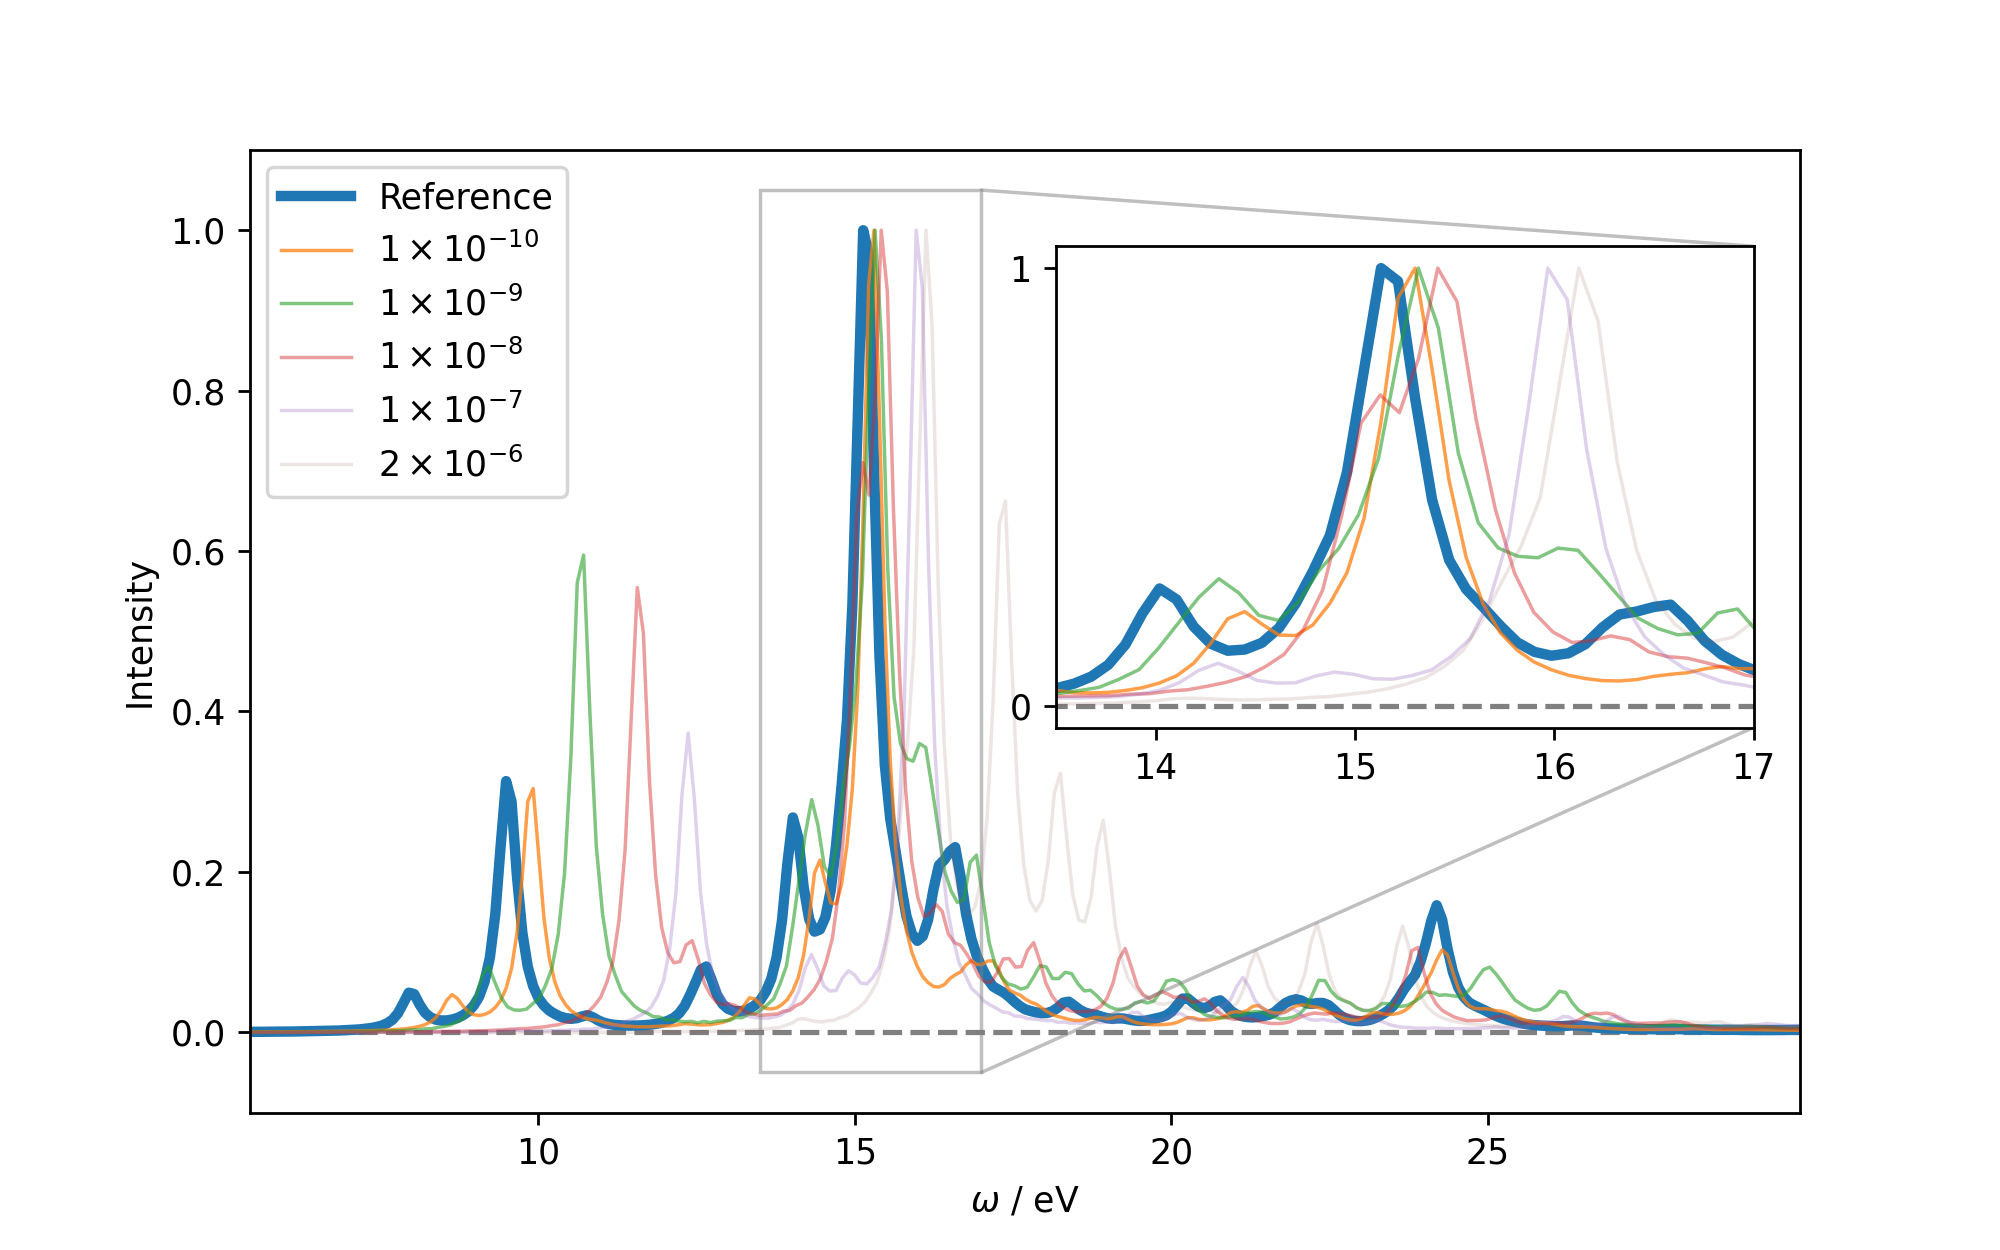
\includegraphics[scale=.6]{p3/figures/pno_abs.png}
    \caption{Reference and PNO absorption spectra for five cutoffs: 
    [$1\times 10^{-10}$, $1\times 10^{-9}$, $1\times 10^{-8}$, $1\times 10^{-7}$, 
    $2\times 10^{-6}$] corresponding to [$93\%$, $82\%$, $63\%$, $44\%$, $24\%$]
    of the MO virtual space, respectively.}
    \label{fig:pno_abs}
\end{figure}
%For all truncated PNO virtual spaces considered, the base peak appears to within 1.5 eV of the 
%reference. 
Overall, truncated PNO virtual spaces approximate the position of the base peak well,
with the smallest space predicting a base peak within 1.5 eV of the reference,
and the two largest spaces predict this peak to within 0.2 eV of the reference.
Convergence to the reference base peak occurs from the right, indicating
a lowering of excited state energies as the size of the virtual space increases. 
This trend can also be seen for the smaller peak near 10 eV. However, convergence of the shoulder 
peaks on either side of the base peak, indicated by the inset of 
Figure~\ref{fig:pno_abs}, is less predictable. Even the largest spaces considered
do not correctly predict the excitation energy, with no clear advantage to having
93\% of the virtual space as compared to just 83\% for predicting these peaks.
This trend continues into the higher-energy range of the spectrum, with the 
performance of each cutoff being nearly indistinguishable. 

Performance of the PAO space is shown in Figure~\ref{fig:pao_abs}. 
\begin{figure} 
    \centering
    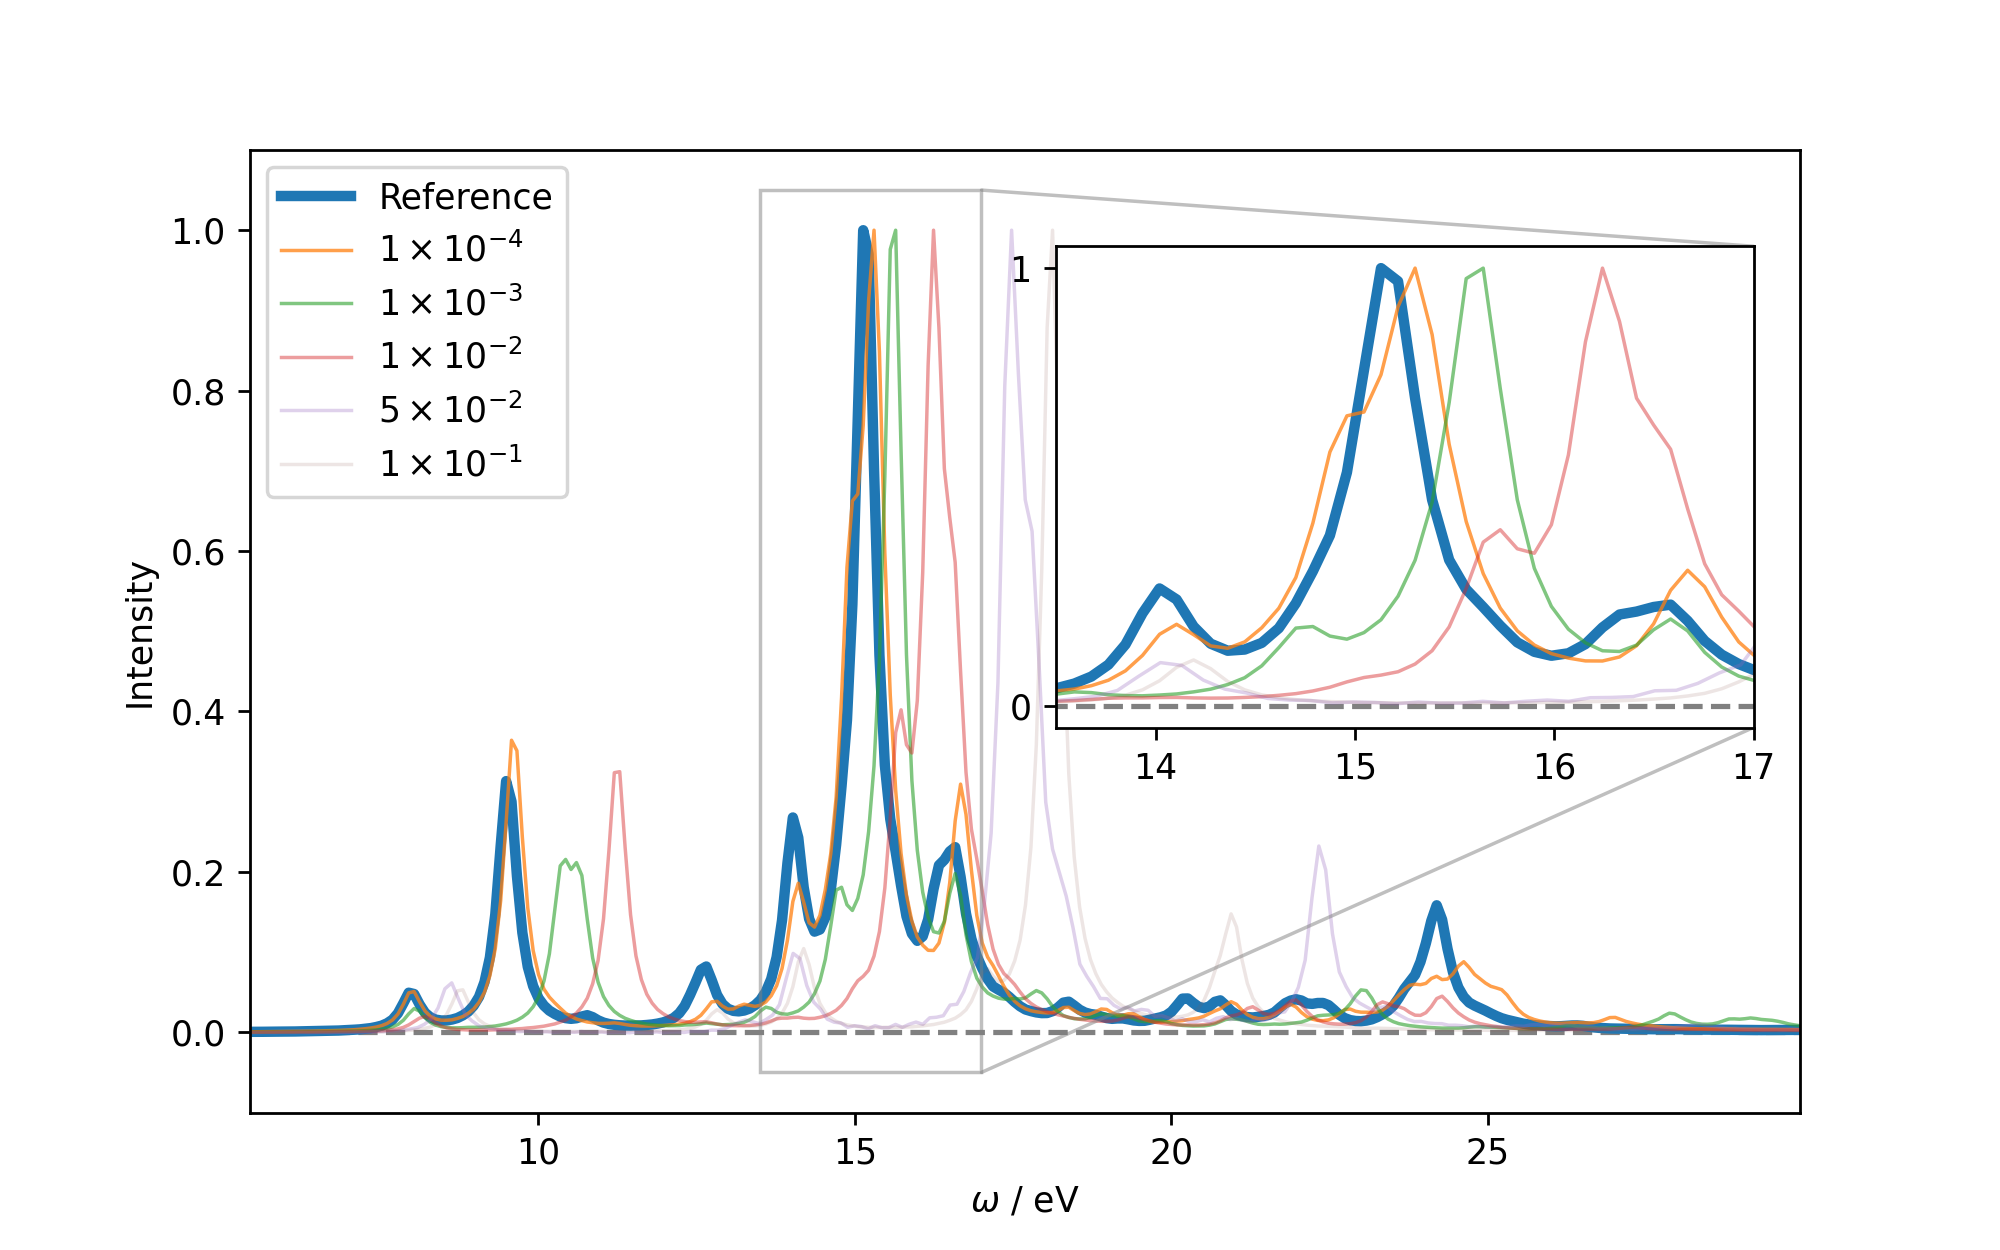
\includegraphics[scale=.6]{p3/figures/pao_abs.png}
    \caption{Reference and PAO absorption spectra for five cutoffs: 
    [$1\times 10^{-4}$, $1\times 10^{-3}$, $1\times 10^{-2}$, $5\times 10^{-2}$, 
    $1\times 10^{-6}$] corresponding to [$95\%$,$86\%$,$63\%$,$46\%$,$23\%$]
    of the MO virtual space, respectively.}
    \label{fig:pao_abs}
\end{figure}
The largest truncated PAO virtual space, on average 95\% of the MO space, accurately 
predicts the excitation energies for each major peak below 17 eV. Particularly around 10 eV, 
this is noticeably improved performance relative to the largest PNO space tested, 
with only a 2\% difference in the average size of the virtual space. 
However, accuracy rapidly declines even at 86\% of the virtual space, where the base peak
position is already worse than what was predicted with a PNO space of just 63\% of the 
MO space. Performance continues to degrade as energy increases and the average size of 
the PAO space decreases. For the final two cutoffs, at averages of 46\% and 23\% of the
MO space, the base peaks are 3 eV or more away from the reference, and no peak is 
exhibited near 25 eV. These spaces also fail to predict the second largest peak, the 
excitation just below 10 eV. 

\subsubsection{ECD} \label{sss:ecd}
Overall, neither scheme produced adequate results upon truncation of the virtual space. 
This result is not entirely surprising -- in studies of local correlation applied to 
response theory by Crawford \textit{et al}., 
\cite{McAlexander2016,Kumar2017,Crawford2019,DCunha2021} 
traditional schemes proved inaccurate for another 
electric dipole--electric dipole property, the electric polarizability.
In terms of response theory,
the polarizability (and the refractive index) is related to the \textit{real} part 
of the electric dipole--electric dipole linear response tensor 
($\boldsymbol{\alpha}_{ij}$ in Eq.~(\ref{eq:mu_exp})), 
while absorption
is related to the \textit{imaginary} part. Indeed, all linear absorptive properties
such as absorption and CD 
are related to the imaginary component of a linear response tensor, while dispersive 
properties such as refractive index and 
circular birefringence (also known as optical rotation)
are related to the real component.
\cite{Barron2004,Norman2011}
To continue, we will look at another absorptive property which is related to the mixed
electric dipole--magnetic dipole linear response tensor -- ECD.

The ECD spectrum is obtained from the Fourier transform of Eq.~(\ref{eq:ecd}).
Being a bisignate, mixed-response property, ECD is a considerable computational
challenge, similar to its dispersive counterpart circular birefringence. 
Figure~\ref{fig:pno_ecd} shows the results for an ECD spectrum in the same PNO 
orbital spaces used in the previous section.
\begin{figure} 
    \centering
    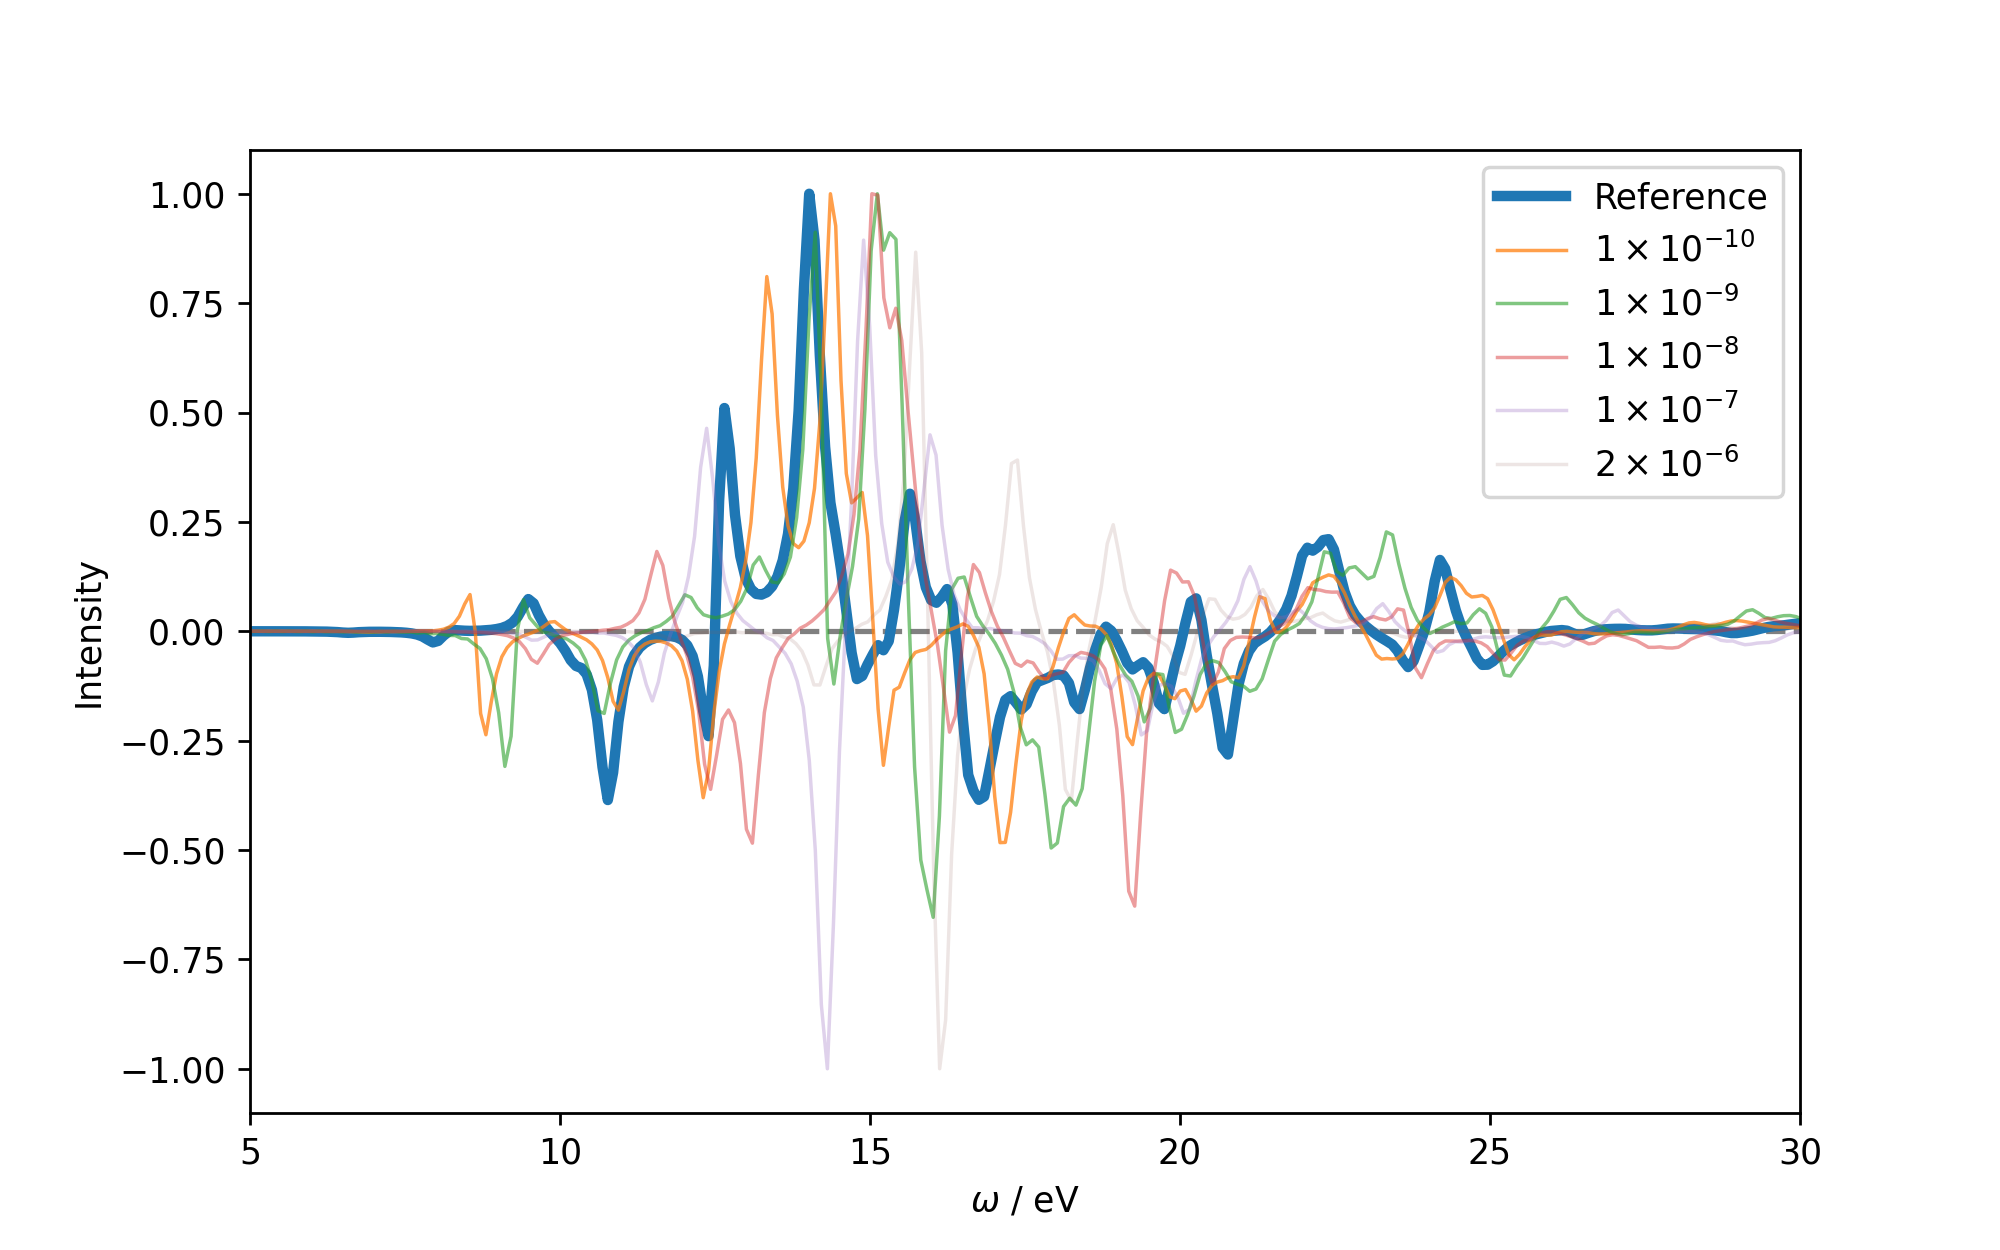
\includegraphics[scale=.6]{p3/figures/pno_ecd.png}
    \caption{Reference and PNO ECD spectra for five cutoffs: 
    [$1\times 10^{-10}$, $1\times 10^{-9}$, $1\times 10^{-8}$, $1\times 10^{-7}$, 
    $2\times 10^{-6}$] corresponding to [$93\%$,$82\%$,$63\%$,$44\%$,$24\%$]
    of the MO virtual space, respectively.}
    \label{fig:pno_ecd}
\end{figure}
The dynamic response of the magnetic dipole to the electric field in this frequency 
range is considerably more complicated than that of the electric dipole. Below 60\% of
the MO space, virtually all distinguishing characteristics of the reference 
spectrum are unidentifiable. Further, at 82\%, the base peak appears to be a pair of 
peaks, more resembling the pair of peaks appearing just above 15 eV in the 
reference spectrum, with the major peak just below 15 eV being the second strongest.
At an average of 93\%, the overall \textit{shape} of the spectrum in the 10 eV to 
20 eV range more closely resembles that of the reference; however, the excitation
energies are, in some cases, even less accurate than those of smaller PNO spaces.
The trend of lowering excited state energies with increased virtual space seen in 
Section~\ref{sss:ecd} is no longer discernible. 

As in the case of absorption, the PAO basis is not noticeably more efficient at
approximating the full MO space than the PNO space. Figure~\ref{fig:pao_ecd} 
shows the results using the same truncated PAO spaces as in Section~$\ref{sss:abs}$.
\begin{figure} 
    \centering
    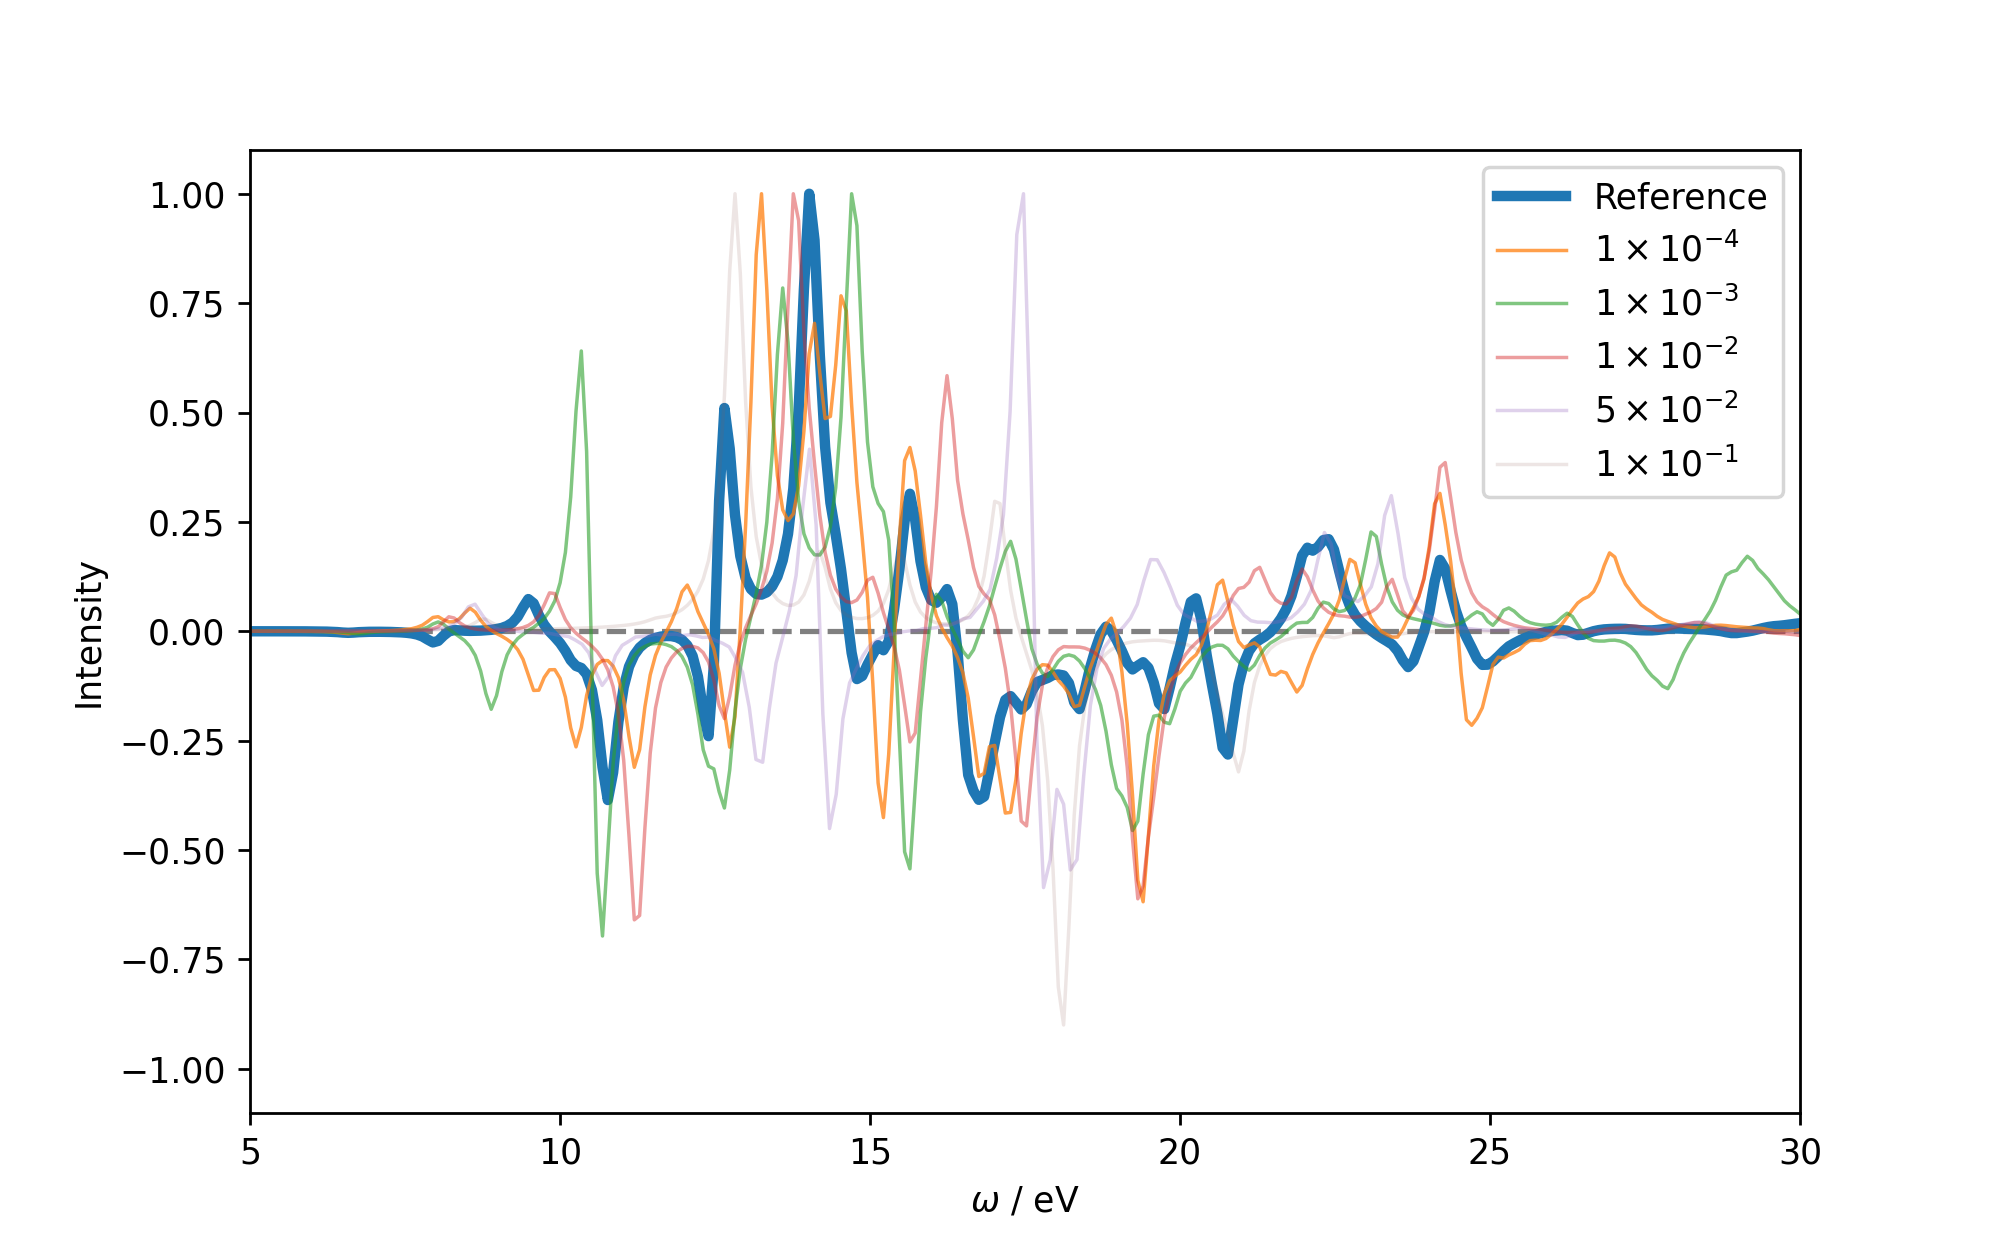
\includegraphics[scale=.6]{p3/figures/pao_ecd.png}
    \caption{Reference and PAO ECD spectra for five cutoffs: 
    [$1\times 10^{-4}$, $1\times 10^{-3}$, $1\times 10^{-2}$, $5\times 10^{-2}$, 
    $1\times 10^{-6}$] corresponding to [$95\%$,$86\%$,$63\%$,$46\%$,$23\%$]
    of the MO virtual space, respectively.}
    \label{fig:pao_ecd}
\end{figure}
The performance of the PAO basis near the base peak varies wildly with truncation,
as in the PNO case. In the low-frequency region, the PAO results are considerably 
worse -- see the two negative peaks between 10 eV and 15 eV. Curiously, the 
largest PAO spaces considered predict significant peaks above 25 eV that are not 
present in the reference, any of the PNO spaces tested, or the smaller PAO
spaces. This suggests a strong sensitivity of the response of the wave function
to the completeness threshold used for determining the occupied domains.
%fundamentally different electronic structure in the
%presence of the perturbing field, which is a direct result of the charge-based 
%completeness threshold used for determining the occupied domains.
%albeit at very large frequencies which are of little practical use.

\subsection{Amplitude Dynamics} \label{ss:amps}
As evidenced by the preceding data, the truncated PNO and PAO virtual spaces do not
efficiently model the wave function in the presence of a perturbing EMF. As noted in
Section~\ref{sss:abs}, these shortcomings are well-documented in the case of response
theory. However, a real-time formalism offers the opportunity to analyze the wave 
function in great detail over time, perhaps shedding light on \textit{where} and 
\textit{how} the locally correlated wave functions are deficient. The following
section will scrutinize the $t_\mu$ and $\lambda_\mu$ amplitudes of 
Eqs.~(\ref{eq:t_mu}) and (\ref{eq:l_mu}), respectively, in hopes of determining the 
important fluctuations in the wave function and whether these spaces sufficiently 
capture these changes.

Response to external perturbations by the CC amplitudes give rise to
dynamic energetics and properties. In the past, distributions of perturbed amplitudes
(relative to their ground-state counterparts) have been used to justify the 
difficulty in computing response functions with local correlation methods in the 
frequency domain. 
\cite{McAlexander2016,Crawford2019,DCunha2021} 
However, initial findings show that in RTCC, the relative distribution of amplitudes 
by magnitude is not significantly impacted.\cite{Crawford2019} 
Despite this, typical means of exploiting amplitude
sparsity have been shown to be inefficient by the preceding sections. 
First, to understand the response of 
the amplitudes to the external perturbation, we plot the 
change in the norm of the amplitude tensors relative to the ground-state amplitudes 
as a function of time in Figure~\ref{fig:norm}.
\begin{figure} 
    \centering
    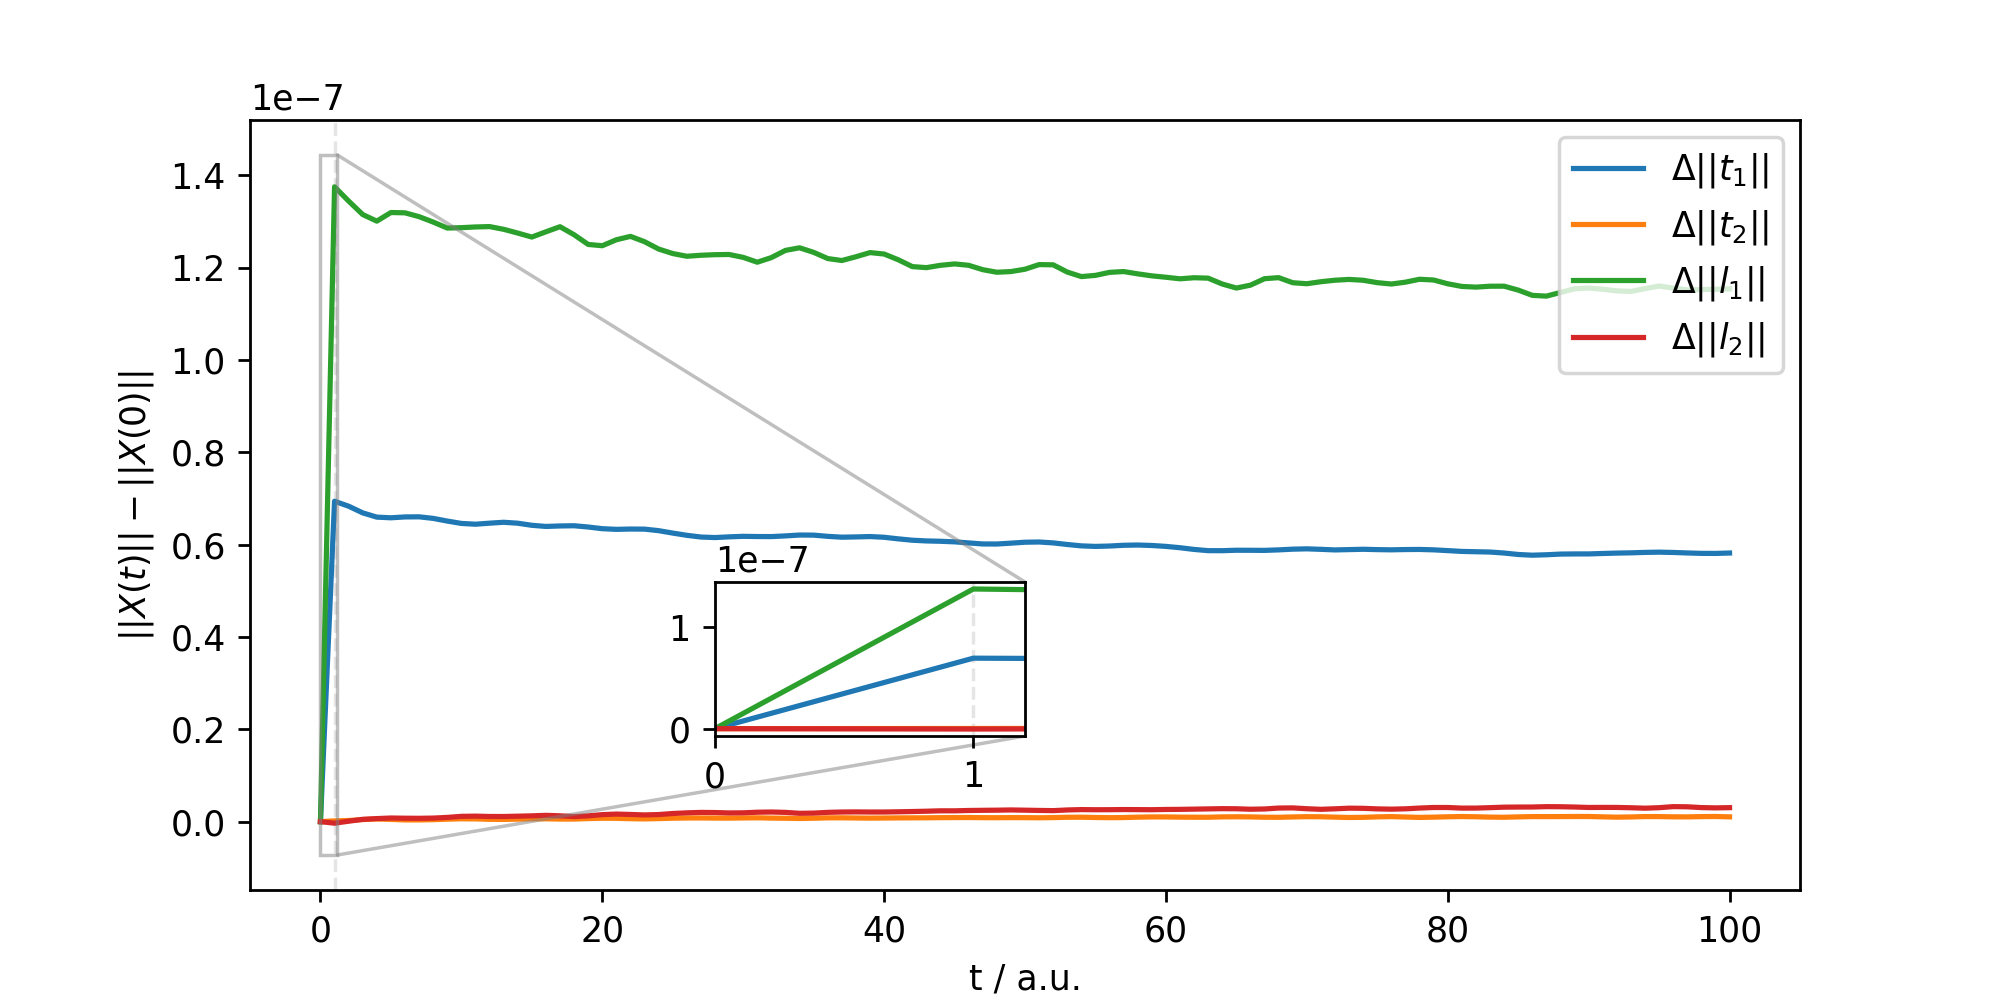
\includegraphics[scale=.6]{p3/figures/amp_norm.png}
    \caption{Time-dependent change in the norm of the amplitude 
    tensors relative to the ground-state amplitudes.
    (Field and step parameters remain unchanged, and 
    the amplitude norm is taken at every 1 a.u.)}
    \label{fig:norm}
\end{figure}
Results for the untruncated PNO and PAO spaces are identical to those
for the MO space, as the unitary transformations resulting from untruncated localized virtual spaces
in Eqs.~(\ref{eq:rotate}) preserves the tensor norm.
Amplitude norms from propagations carried out in truncated PNO and PAO spaces
are nearly indistinguishable (see SI).

Figure~\ref{fig:norm} shows that the magnitude of the response by the wave function
is predominantly within the singles amplitudes $t_1$ and $\lambda_1$. This is 
consistent with the notion that singles are paramount for the computation of 
response properties.\cite{Christiansen1995,Koch1997} However, the form of Eq.~(\ref{eq:pair_D})
does not include any contributions by singles, due to being built from MP2-level
amplitudes where singles do not contribute until at least the second order 
in the wave function and fourth order in the energy. This suggests that even in schemes
which seek to include the EMF perturbation in the construction of the reduced virtual space,
such as PNO++,\cite{DCunha2021} response of the singles should be considered.

Aside from the matrix norm, we can also inspect the individual amplitudes to track
their evolution in time. The heat maps in Figure~\ref{fig:amps} show the difference 
in $t_1$ amplitudes, relative to the ground state, for three time steps selected 
from the first 100 a.u. of the simulation.
\begin{figure}
    \begin{subfigure}{.5\textwidth}
        \centering
        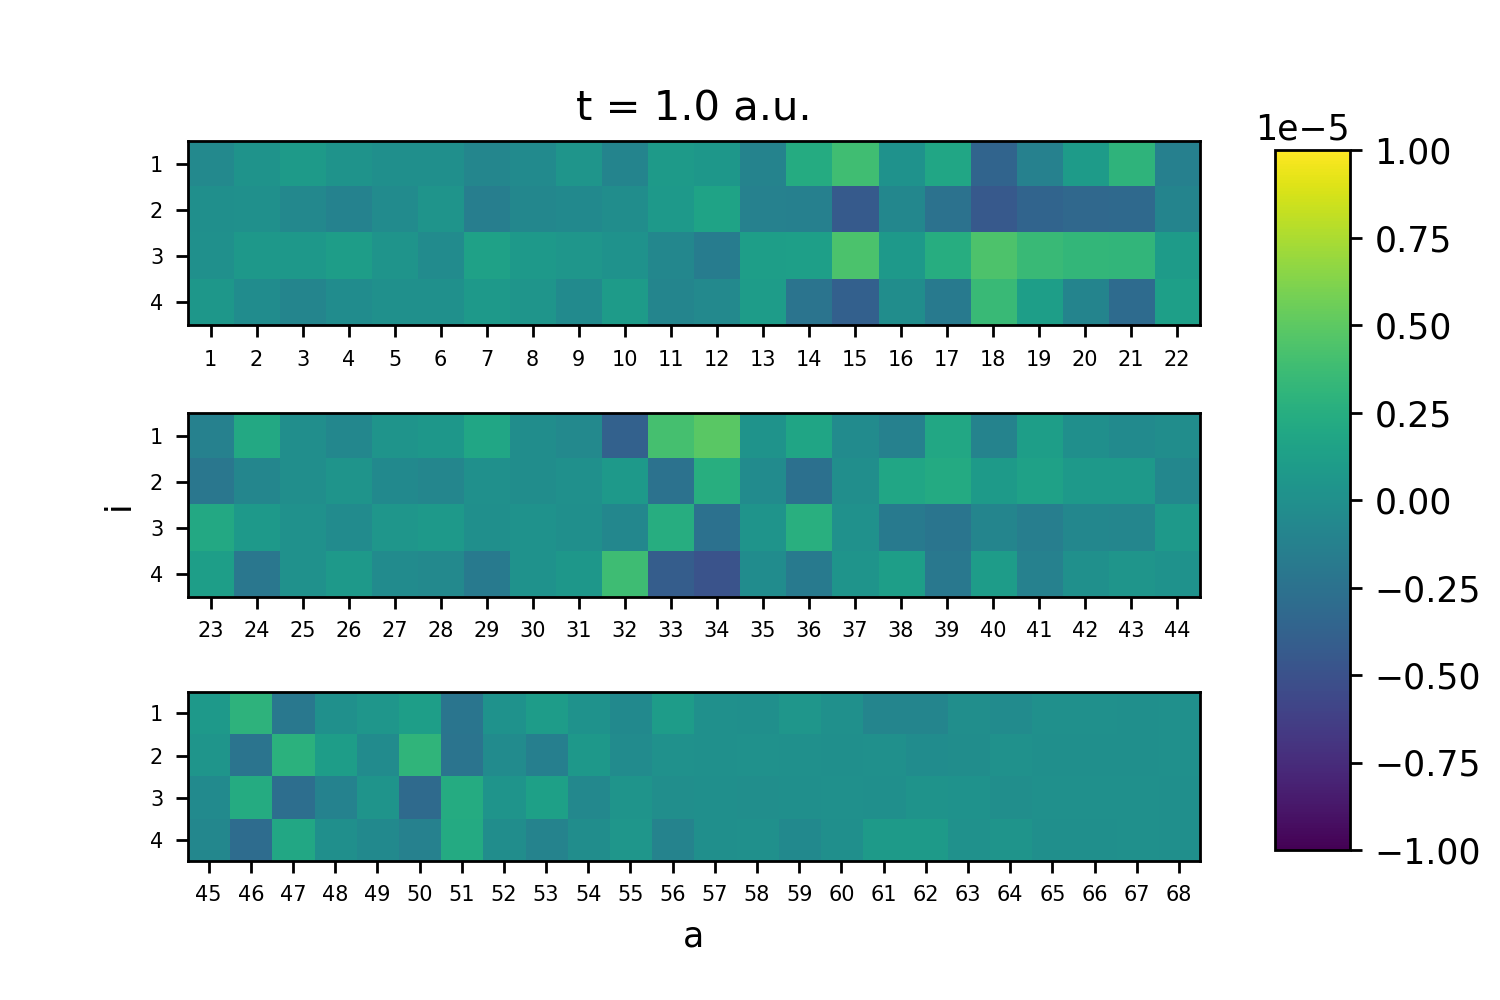
\includegraphics[scale=0.5]{p3/figures/MO_delta_t1_1.png}
        \caption{}
        \label{fig:MO_t1_1}
    \end{subfigure}%
    \begin{subfigure}{.5\textwidth}
        \centering
        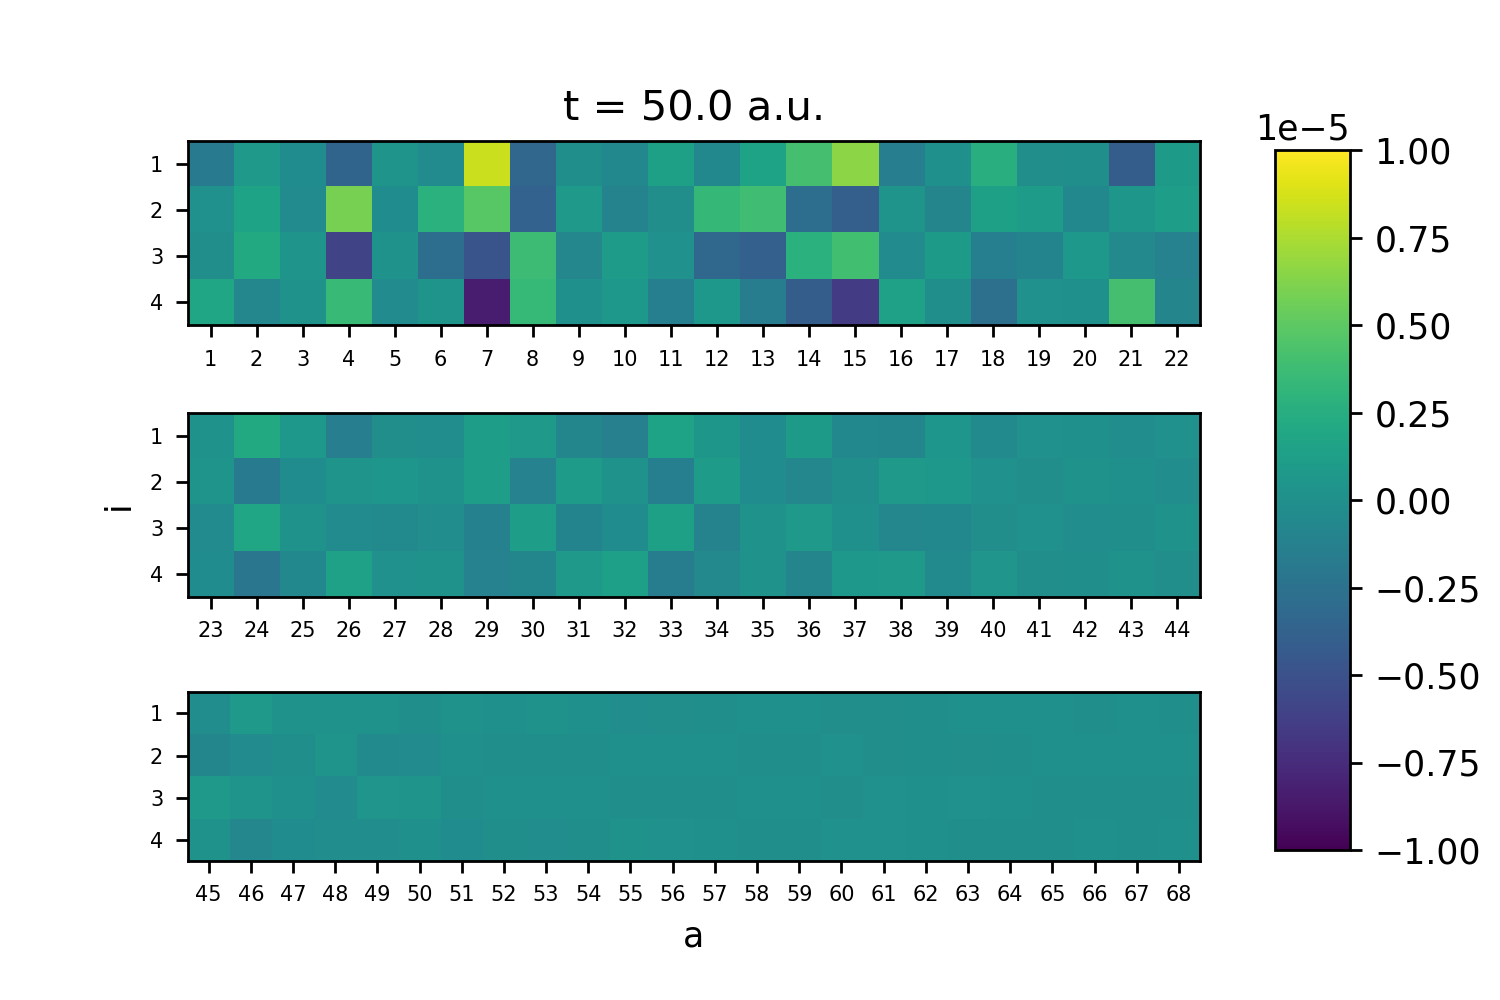
\includegraphics[scale=0.5]{p3/figures/MO_delta_t1_50.png}
        \caption{}
        \label{fig:MO_t1_50}
    \end{subfigure}
    \begin{subfigure}{.5\textwidth}
        \centering
        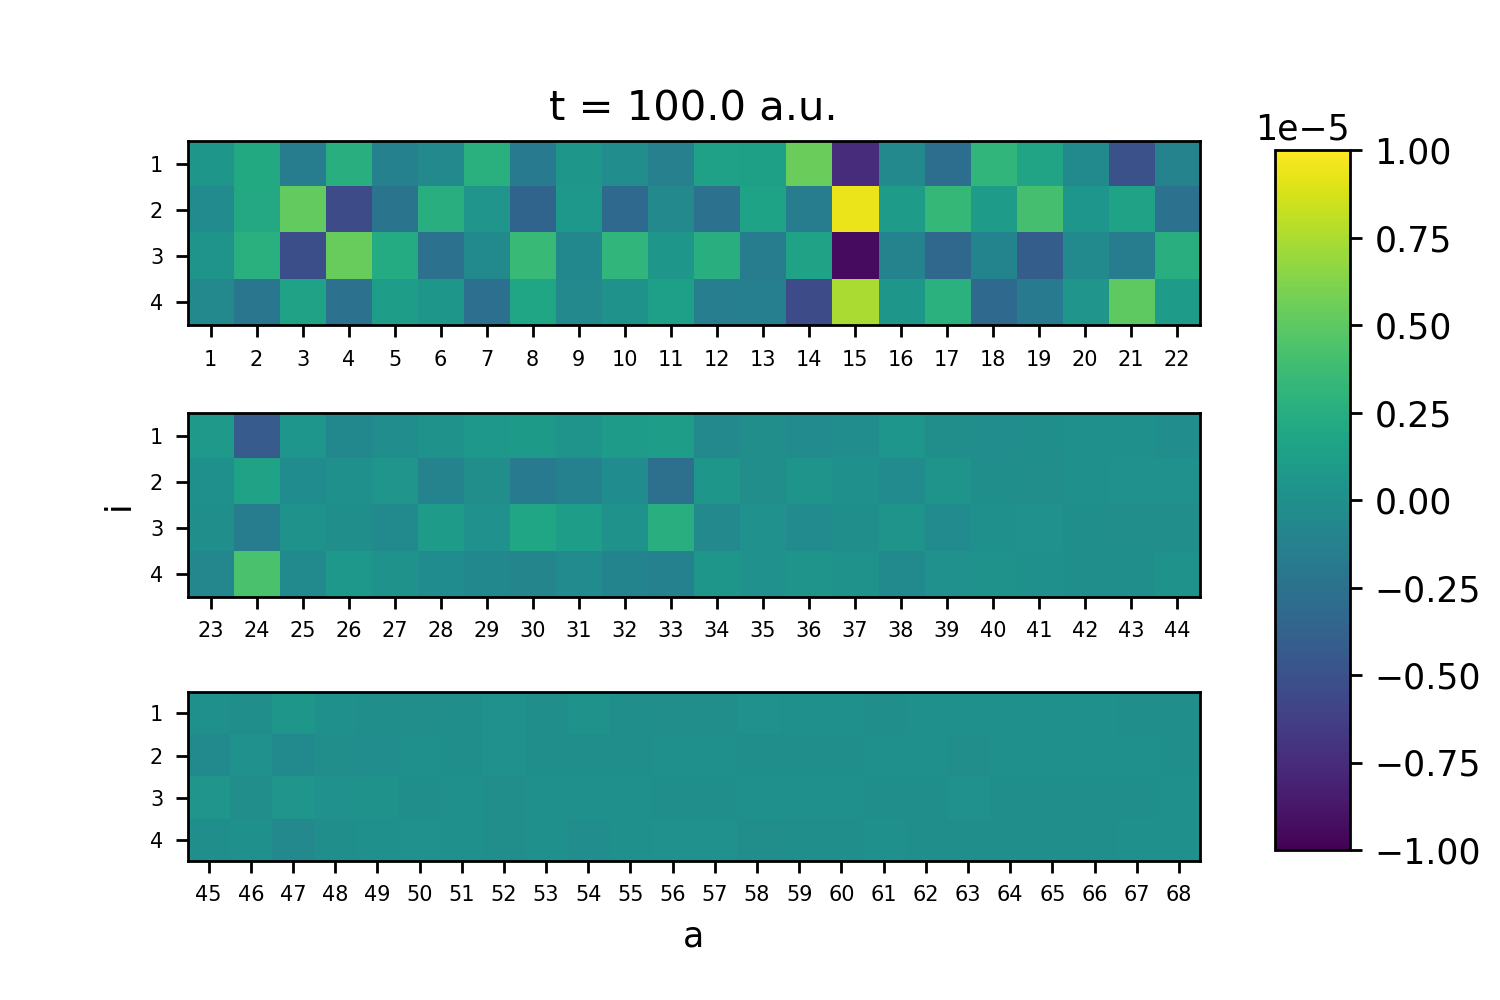
\includegraphics[scale=0.5]{p3/figures/MO_delta_t1_100.png}
        \caption{}
        \label{fig:MO_t1_100}
    \end{subfigure}
    \caption{MO-basis $t_1$ amplitude deviations from $t = 0$ after (a) 1 a.u., (b) 50 a.u., and 
    (c) 100 a.u. of time propagation. Each row contains the same four occupied orbital indices
    and a subset of virtual indices as indicated by the x-axis labels.}
    \label{fig:amps}
\end{figure}
The amplitudes are ordered by the orbital energies of the associated MOs. 
The amplitudes which experience significant oscillations vary throughout the simulation,
though there are several discernible trends. First, most large amplitude deviations
are associated with all occupied orbitals simultaneously. This is due to the relatively small size of 
the system, with only four occupied orbitals, all of which are likely important in the
description of the ground- and excited-state wave functions. Secondly, 
at any given time during the propagation,
a large number of amplitudes have not significantly deviated from their ground state values.
This supports the notion
that relative sparsity is maintained within the amplitudes throughout the simulation,
but this sparsity is distributed differently throughout the amplitude tensors as
the wave function is propagated.  

A third trend is that amplitudes which respond strongly tend to be associated with 
low-energy virtual orbitals. Chemical intuition would suggest that energetically 
low-lying molecular orbitals will be the most involved in electronic excitations.
However, while amplitude responses are indeed larger for lower-energy virtual orbitals, 
smaller amplitude 
deviations in Figure~\ref{fig:amps} extend far into the virtual space. This explains
the difficulty of simply truncating with respect to orbital energy: the 
high-energy MOs are still important to the time-evolution of the wave function 
in the presence of an EMF. 

Figure~\ref{fig:pno_amps} shows the $t_1$ amplitudes for the same simulation,
rotated into the untruncated PNO basis using $Q_{ii}$ as defined in
Eq.~(\ref{eq:Q_pno}).
\begin{figure}
    \begin{subfigure}{.5\textwidth}
        \centering
        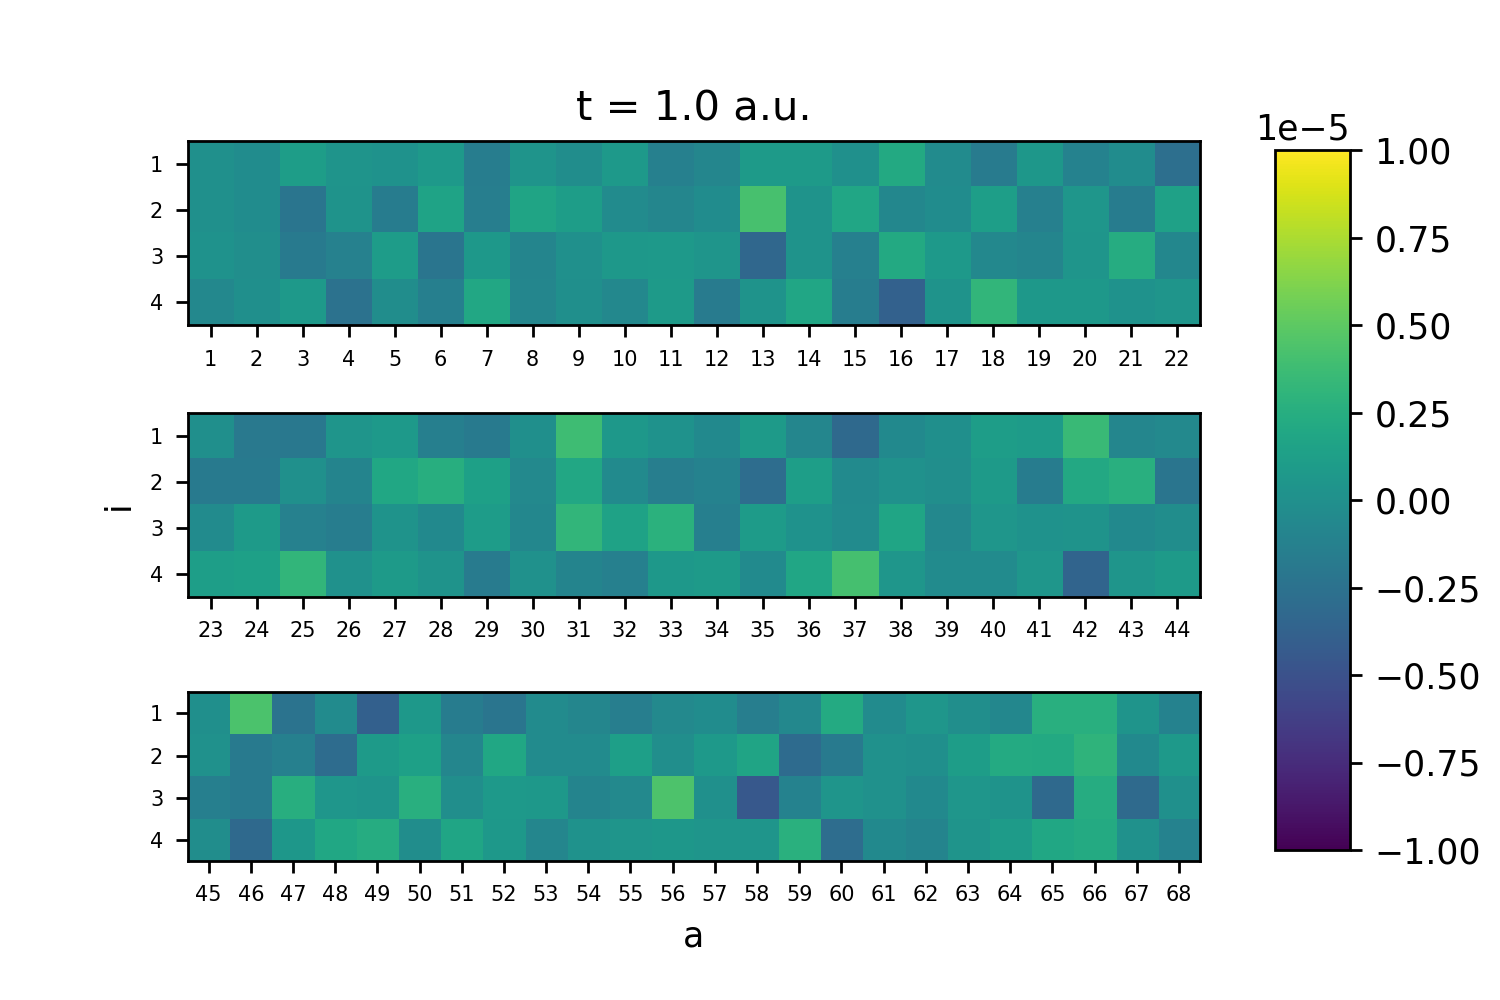
\includegraphics[scale=0.5]{p3/figures/PNO_delta_t1_1.png}
        \caption{}
        \label{fig:PNO_t1_1}
    \end{subfigure}%
    \begin{subfigure}{.5\textwidth}
        \centering
        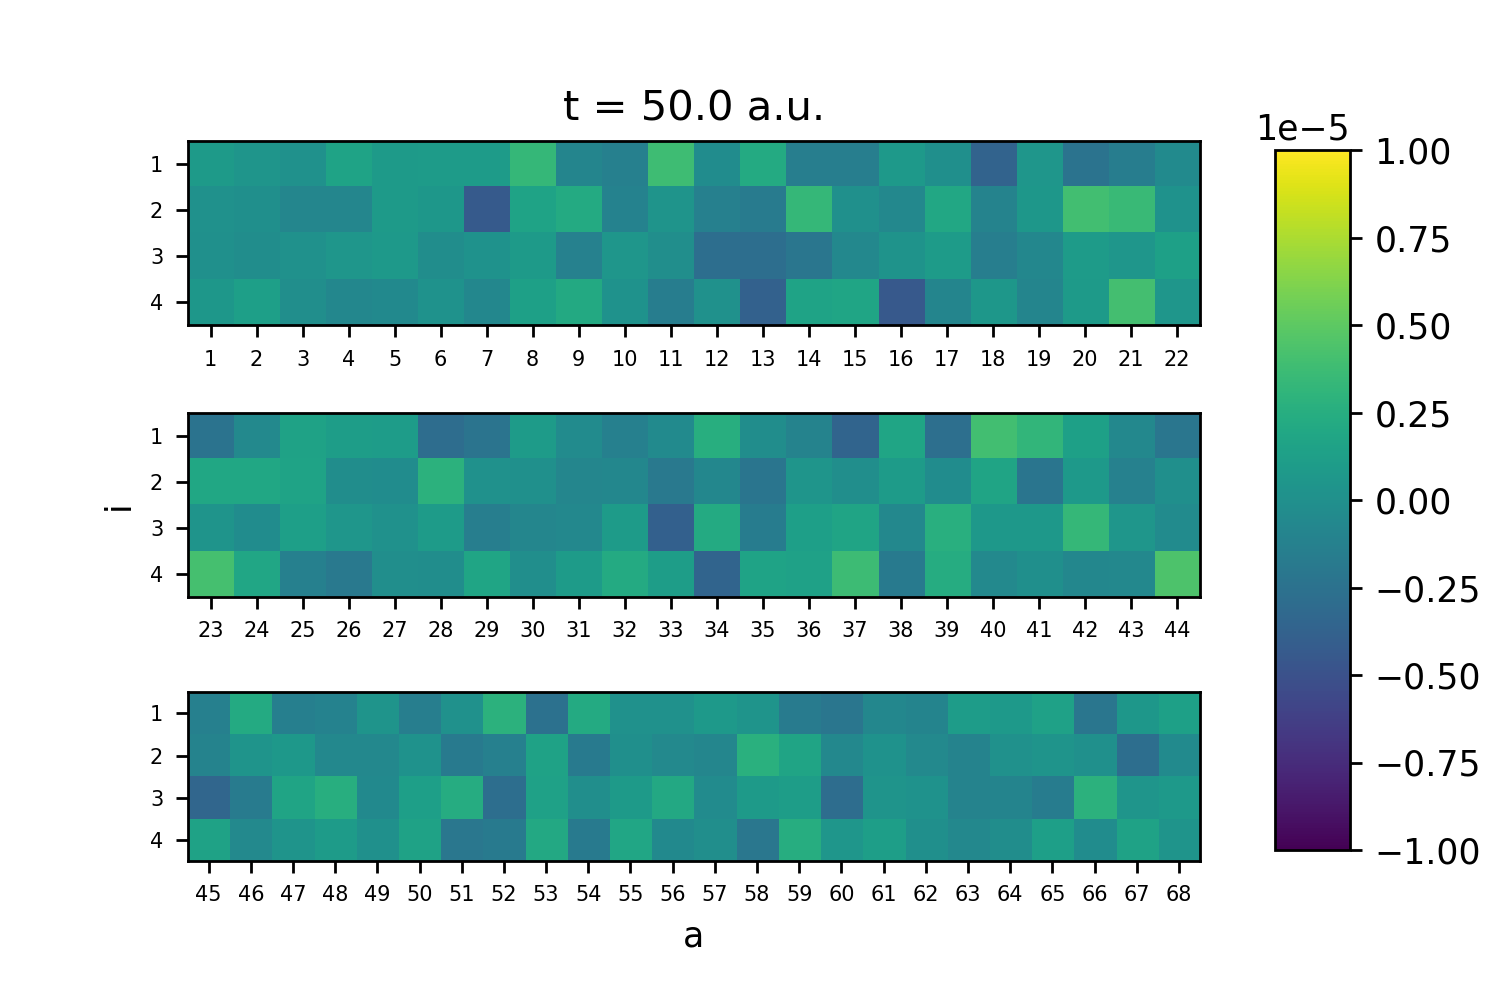
\includegraphics[scale=0.5]{p3/figures/PNO_delta_t1_50.png}
        \caption{}
        \label{fig:PNO_t1_50}
    \end{subfigure}
    \begin{subfigure}{.5\textwidth}
        \centering
        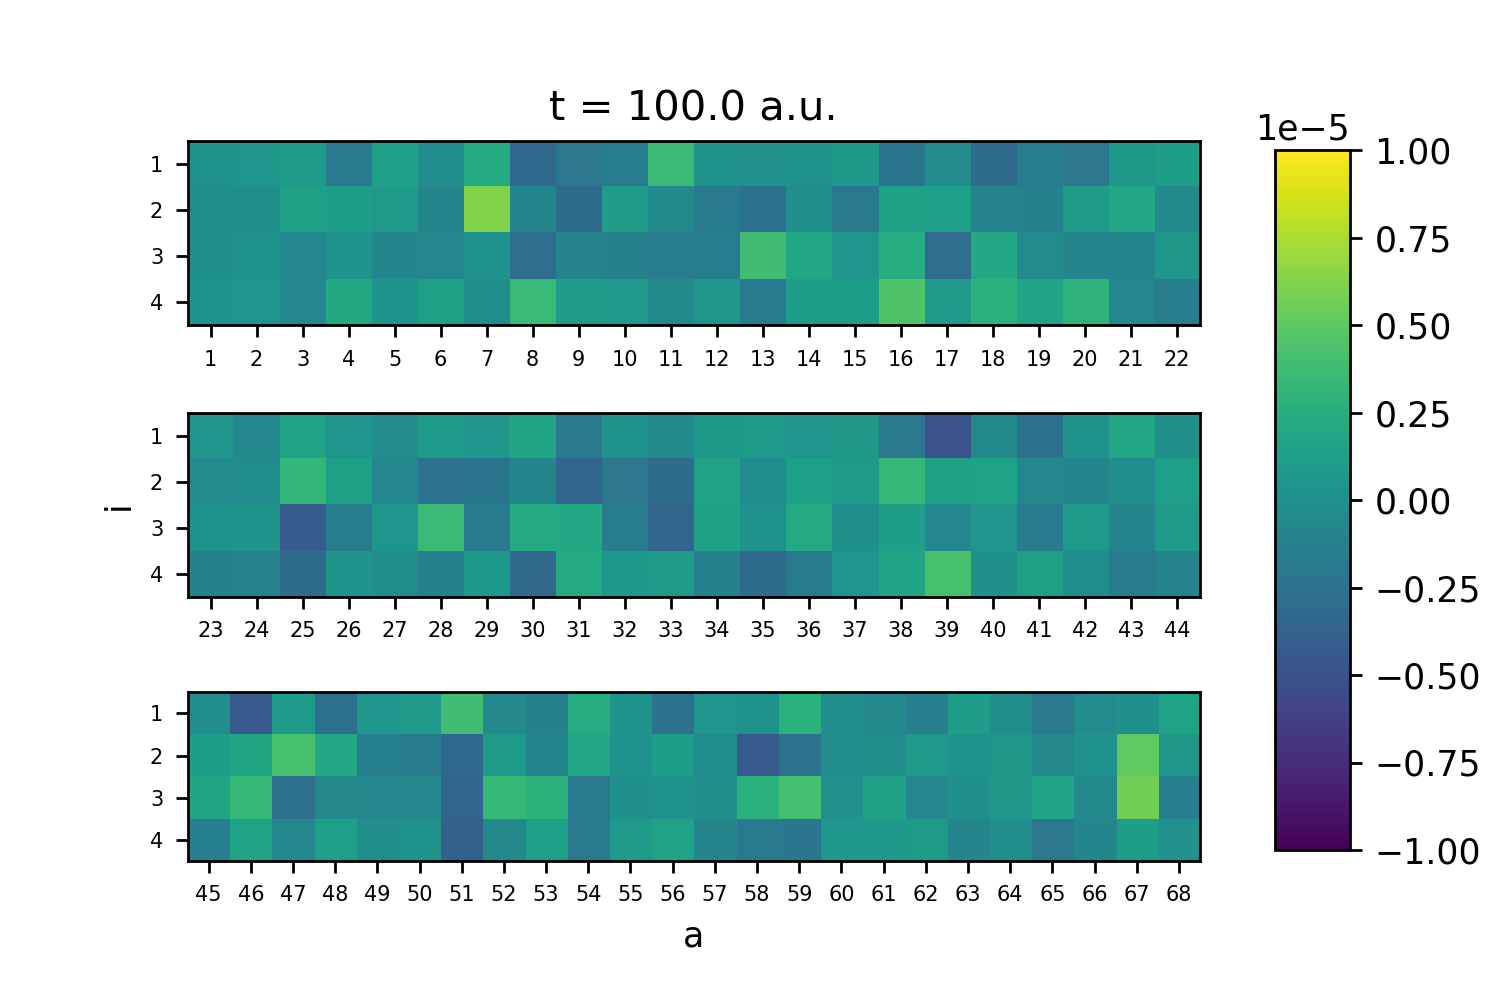
\includegraphics[scale=0.5]{p3/figures/PNO_delta_t1_100.png}
        \caption{}
        \label{fig:PNO_t1_100}
    \end{subfigure}
    \caption{PNO-basis $t_1$ amplitude deviations from $t = 0$ after (a) 1 a.u., (b) 50 a.u., and 
    (c) 100 a.u. of time propagation. Each row contains the same four occupied orbital indices
    and a subset of virtual indices as indicated by the x-axis labels.}
    \label{fig:pno_amps}
\end{figure}
(It should be noted that, due to redundancy in the AO-based virtual 
spaces for each pair, PAO-basis amplitudes cannot be compared directly in 
this manner.)
It can be immediately seen that the amplitude deviations
are less sparse in the PNO basis after the application of the EMF. 
Many more amplitudes exhibit
perceivable differences, and strong deviations (magnitudes approaching 
$1\times 10^{-5}$) are no longer present. This is a clear demonstration
of the issue with truncating orbital spaces based on the present criterion ---
rather than exploiting sparsity, the amplitude tensors have become less sparse.
It may also suggest a recipe for building a more appropriate 
virtual space for truncation. 
In the following section, we propose some alternative schemes based on the 
literature and the results of this study.
%In the following section, we compare a selection
%of orbitals which correspond to strong amplitude deviations in the MO basis 
%(specifically virtuals 3, 4, 7, and 15)
%based on orbital spatial extent to determine if this may be a possible criterion 
%for truncation of the virtual space.

\subsection{Possible Alternatives} \label{ss:alt}
\begin{figure}
    \centering
    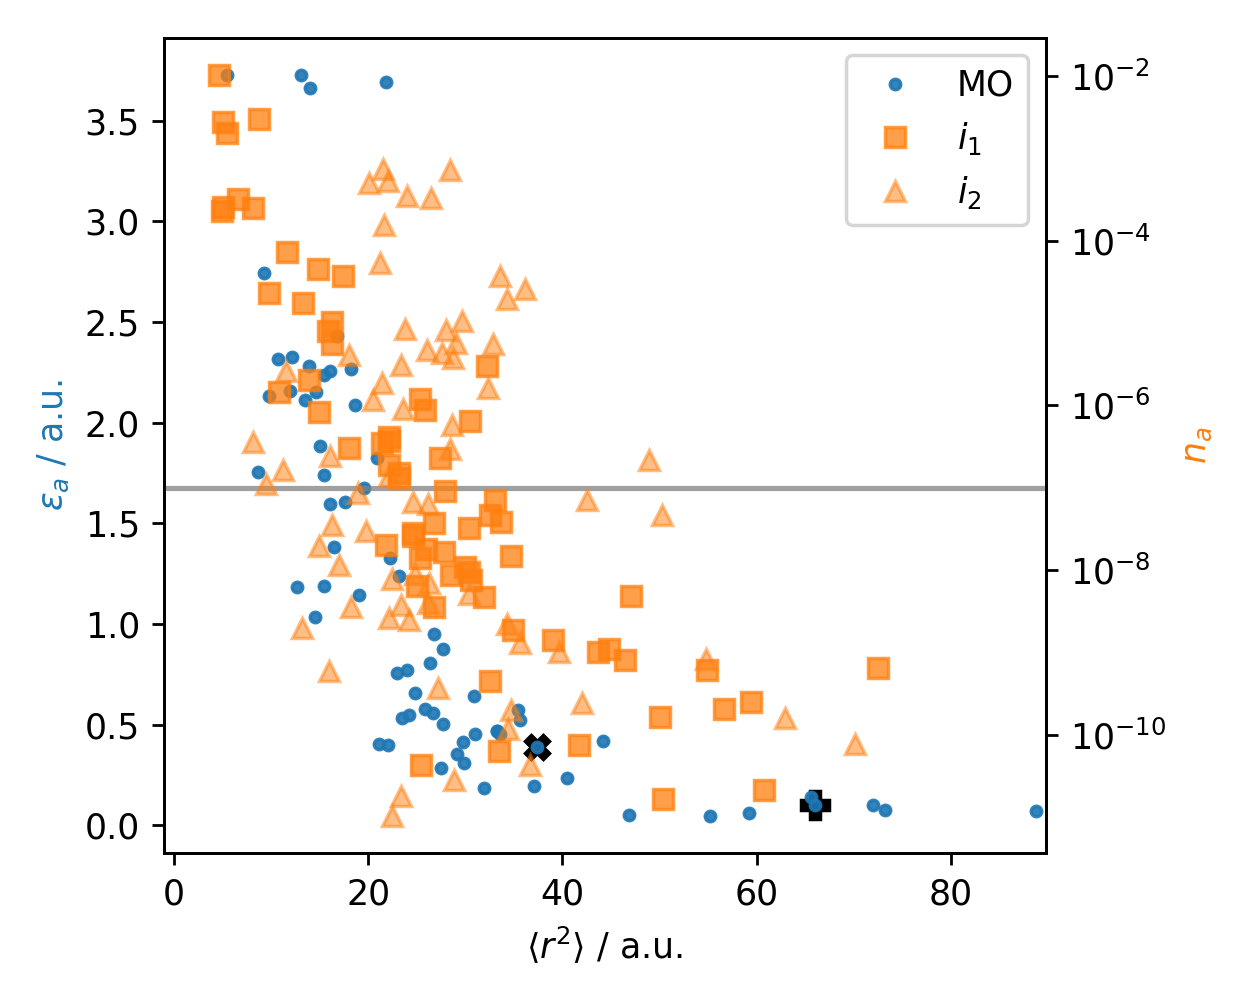
\includegraphics[scale=0.75]{p3/figures/extent.png}
    \caption{Virtual MO energy $\epsilon_a$ and the
    occupation number $n_a$ (plotted on a log scale)
    for unique PNO spaces $i_1$ and $i_2$ 
    versus orbital extent in arbitrary units.
    Virtual MOs 7 and 15 are denoted by a solid $\boldsymbol{+}$ 
    and $\boldsymbol{\times}$, respectively.
    The horizontal line denotes a PNO cutoff 
    of $1\times 10^{-7}$.}
    \label{fig:extent}
\end{figure}
Figure~\ref{fig:extent} shows the virtual MO energy $\epsilon_a$ and the 
PNO occupation number $n_a$ plotted against the orbital extent
$\langle r^2 \rangle$ in arbitrary units. 
In the PNO basis, a unique virtual space is prepared
for every occupied pair, resulting in 16 unique spaces for the four occupied
spatial orbitals $i$. However, for transforming
a single orbital index, we only require the diagonal rotation matrices,
\textit{i.e.}, $Q_{ii}$. There are four such spaces; however, by symmetry,
only two are unique. Both are included in Figure~\ref{fig:extent}. 

Truncation of the PNO space begins from the bottom of Figure~\ref{fig:extent}. 
At an occupation number cutoff of $1\times 10^{-7}$ (indicated by a horizontal
line), all orbitals below this line are neglected in the PNO space. Roughly
66\% of the virtual space lies in this region. From these data, it is clear
that even modest truncation of the virtual space neglects the diffuse 
regions of the wave function, which are important for excited-state
properties in systems with significantly delocalized characteristics,
such as systems containing Rydberg-type excitations.

%Table~\ref{ta:ext} reports the orbital extent $\langle r\rangle$ for virtual orbitals $a$
%corresponding to four of the strongest deviations in Figure~\ref{fig:amps}. 
%These orbitals are labeled 4, 7, 8, and 15, in
%both the MO and PNO basis. In the PNO basis, a unique virtual space is prepared
%for every occupied pair, resulting in 16 unique spaces for the four occupied
%spatial orbitals $i$. However, for transforming
%a single orbital index, we only require the diagonal rotation matrices,
%\textit{i.e.}, $Q_{ii}$. There are four such spaces; however, by symmetry, the domains of occupied
%orbitals 1 and 4 are the same, as are 2 and 3. Thus, orbital extents for only those
%two unique orbital spaces $i_1$ and $i_2$  are shown.
%\begin{table}
%    \centering
%    \begin{tabular}{|c|c|c|c|}
%        \hline
%%        $a$ &   MO  &   PNO   &        \\  
%        $a$ &  MO  &   \multicolumn{2}{c|}{PNO} \\  
%        \hline
%%        \multicolumn{2}{|c|}{}  & $i_1$   & $i_2$  \\ 
%            &       & $i_1$   & $i_2$  \\
%        \hline
%%         3  & 59.23 & 7.9     & -24.67 \\ 
%%        \hline
%         4  & 88.76 & -13.08  & -3.13  \\ 
%        \hline
%         7  & 66.00 & 0.73    & -0.07  \\ 
%        \hline
%         8  & 65.56 & -3.91   & -10.35 \\ 
%        \hline
%         15 & 37.39 & -15.11  &  1.32  \\
%        \hline
%    \end{tabular}
%    \caption{Orbital spatial extent of four selected virtual orbitals in the MO
%    and PNO spaces.}
%    \label{ta:ext}
%\end{table}
%A full table of virtual orbital extents can be found in the SI. 
%In the MO basis, the orbitals in Table~\ref{ta:ext} 
%correspond to the strongest amplitude deviations in Figure~\ref{fig:amps}.
%These are also some of the most diffuse orbitals in this basis,
%far larger than the average orbital extent of 26.62.
%As expected, the spatial extent of the PNOs built upon the MOs
%are much more localized. This shows that, in the MO basis,
%strong deviations are predominantly exhibited by amplitudes 
%corresponding to virtual orbitals with a larger spatial extent,
%creating sparsity. In the PNO basis, however, the deviations 
%are evenly spread across a large number of amplitudes corresponding
%to orbitals with relatively small spatial extent, resulting in 
%less sparsity in the amplitude tensor. 
%These findings suggest that virtual domains built for excited state
%properties should seek to include orbitals with large spatial extent,
%and any truncation criterion should preserve these orbitals.

Spatial extent alone may not be a suitable criterion for truncation -- 
this would have obvious a negative impact on the accuracy of the 
correlation energy, which is inherently local in nature. 
Additionally, Figure~\ref{fig:extent} highlights virtual MOs 7 
($\boldsymbol{+}$) and 15 ($\boldsymbol{\times}$),
which correspond to the strongest deviations in 
Figures~\ref{fig:MO_t1_50} and \ref{fig:MO_t1_100}, respectively.
That these orbitals are of varying extent
demonstrates that both diffuse and contracted orbitals play a role in 
the wave function dynamics.
In order to attain a balanced description of wave function components 
important for both energy and property calculations, the combination 
of appropriately determined spaces such as the combined PNO++ approach
has been fruitful. Still neglected in this approach
are the singles amplitudes, which are absent in the MP2 wave functions
used to approximate the occupied pair domains. Schemes to include 
these effects, such as approximate CC2-level $t_1$ guess amplitudes,
may further improve the space and allow greater flexibility for 
truncation. The prospect of utilizing these 
methodologies within the current framework is promising, and work is 
underway to explore their efficiency.

%conc.tex

\section{Conclusions} \label{conc} Here we present the first application
of local correlation to RTCC simulations. The popular PNO and PAO virtual
space localization schemes are applied to the calculation of dynamic electric
and magnetic dipole moments in the presence of an explicit electric field,
providing absorption and ECD spectra, respectively. 
For a helical H$_2$ tetramer, truncation of the
localized virtual space to successively larger fractions of the canonical
virtual space resulted in convergence to the canonical result; however, this
convergence is slow, and errors in excitation energies and intensity are
present even in some of the largest spaces tested, especially for ECD. This
corroborates the results of recent studies applying locally correlated
methods to the prediction of dynamic properties in the frequency domain
using response theory.

%As in the frequency domain, there are a number of possible approaches
%to building a more appropriate virtual space which preserves accuracy in
%response properties upon aggressive truncation. 
Examining the amplitude
dynamics during the propagation, it is shown that the $t_1$ and $\lambda_1$
amplitudes respond most strongly to the field -- a large increase in the
norm of these matrices is observed upon application of the field, followed
by a steady oscillation. The $t_2$ and $\lambda_2$ tensors, by comparison,
remain relatively static throughout. 
These oscillations are largely, but not completely, localized to a selection 
of only a few orbitals, as evidenced by consideration of 
time-dependent deviations in the $t_1$ amplitudes from the ground-state.
In the localized virtual spaces tested,
these oscillations are delocalized throughout the $t_1$ and $\lambda_1$
matrices. 

Orbital extent alone cannot explain the shortcomings of 
the PNO space; however, its effect is significant. 
These results provide an insight into the importance of 
singly-substituted determinants in the time-dependent wave function in the 
presence of an electric field, as well as a potential metric to gauge the 
performance of new localization schemes for frequency- or time-domain 
calculations of dynamic response properties.
In order to attain a balanced description of wave function components 
important for both energy and property calculations, the combination 
of appropriately determined spaces such as the combined PNO++ approach
has been fruitful.\cite{DCunha2021} 
Still neglected in this approach
are the singles amplitudes, which are absent in the MP2 wave functions
used to approximate the occupied pair domains. Schemes to include 
these effects, such as approximate CC2-level $t_1$ guess amplitudes,
may further improve the space and allow greater flexibility for 
truncation. The prospect of utilizing these 
methodologies within the current framework is promising, and work is 
underway to explore their efficiency.


    \chapter{PAPER 3} \label{ch:p3}
%% Introduction

\section{Introduction} \label{se:intro} Dynamic molecular properties induced
by the absorption, scattering, or refraction of an electromagnetic field
(EMF) give rise to a number of experimental techniques for the detailed
investigation and characterization of molecular light-matter interactions
and structure.\cite{Barron2004} Among these properties are absorbance,
circular dichroism (CD), birefringence, Raman scattering, and many more.
These techniques are essential for modern synthetic chemistry in both
research and industrial settings.

Theoretical chemistry has become a ``full partner with experiment''
\cite{Goddard1985} in this regard, providing high-quality benchmark
calculations for affirming or even predicting many molecular properties,
saving time, and increasing certainty in spectral assignments and
molecular structure determination. Computing dynamic properties with
current \textit{ab initio} methods generally involves frequency-domain
perturbation theory, referred to as response theory, to directly calculate
the quantity of interest. \cite{Crawford2006,Norman2011,Helgaker2012}
Coupled cluster (CC) response theory\cite{Koch1990,Pedersen1997} has
emerged as a robust solution to frequency-domain property calculations,
when its cost is not prohibitive.\cite{Crawford2018,Crawford2019} Many
techniques for circumventing the high-degree polynomial scaling of
coupled cluster methods exist, with extensions of these to property
calculations and response theory providing promising results.
\cite{McAlexander2016,Kumar2017,Howard2018,DCunha2021}

However, there are several drawbacks to the response
formalism.\cite{Langhoff,Goings2018,Li2020} First and foremost, the
perturbations must be ``small'' relative to the intramolecular forces
present in the system. This immediately precludes the possibility of
simulating high-energy experiments such as X-ray spectroscopy, which
have numerous applications in materials science and beyond. Second,
only broadband excitations can be modeled straightforwardly: response
theory typically assumes a single, uniform ``kick'' perturbation
across all frequencies. Experimental apparatus, on the other hand,
can make use of complex, multi-phase procedures involving tuned laser
pulses, pump-probe analysis, \textit{etc}.\cite{Maiuri2020} Finally,
temporally controlled multi-photon events such as high harmonic generation
(HHG)\cite{Lewenstein1994,Gorlach} lie outside the realm of the response
formalism. Together, these drawbacks mean a wide variety of experiments
cannot be predicted or supplemented with response theory calculations. To
overcome this, we must move to non-perturbative, time-domain electronic
structure theory, \cite{Goings2018,Crawford2019,Li2020} where there are
fewer limitations on the form of the perturbing EMF.

The alternative of real-time CC (RTCC) methods has been discussed
nearly as far back as the origins of CC itself in the realm of nuclear
physics.\cite{Hoodbhoy1978,Hoodbhoy1979,Gunnarsson78} More recently, a
renewed interest in real-time coupled cluster has developed for the reasons
discussed above. In the past 10 years, several implementations have been
reported, \cite{Huber2011,Kvaal2012,Nascimento2019,Pedersen2019,Park2019}
with new insights into the aspects of numerical
integration\cite{Pedersen2019,Kristiansen2020} and
interpretation\cite{Pedersen2019,Pedersen2021} as
well as applications for a number of spectral properties.
\cite{Nascimento2016,Nascimento2017,Nascimento2019,Park2019,Park2021b}
Orbital adaptive\cite{Kvaal2012} and orbital optimized\cite{Sato2018}
variants have also explored the limitations of unrelaxed canonical
Hartree Fock orbitals, and the effects of alternative reference
orbitals on the propagation of unphysical imaginary components to
energetics and electric dipole moments. 
Notably absent are studies
on the ability to \textit{reduce} the cost of real-time coupled
cluster methods. 
% TDC comment: "Wouldn't Padé approximants fall into this category?"  
% answer: yes, but no one has used Padé for CC yet (to my knowledge) 

Real-time time-dependent density functional theory
(RT-TDDFT) calculations, a cheaper alternative introduced in the 1990s
(then called the \textit{time-dependent local-density approximation}),
\cite{Yabana1996,Yabana1997,Yabana1999,Bertsch2000} have become routine.
\cite{Lopata2011,Castro2015,Tussupbayev2015,Goings2016a,Bruner2016,Goings2018,Sun2019a,Li2020}
Efforts to reduce the cost of RT-TDDFT have largely focused on reducing
simulation time, utilizing techniques such as Pad\'e approximants to
accelerate the convergence of the Fourier transform,\cite{Bruner2016}
and fitting schemes to avoid the Fourier transform all together,
eliminating the problem of short trajectories resulting in low-resolution
spectra.\cite{Ding2013} Repisky \textit{et al.} introduced the concept of 
dipole pair contributions,\cite{Repisky2015,Kadek2015}
which are typically less complicated than the total electric dipole,
and so these may be individually approximated efficiently using the 
techniques mentioned above.   
\cite{Bruner2016} However, the problems of frequency-domain DFT carry
over directly to the time domain, such as the underestimation of excited
state energies\cite{Peach2008} and difficulties arising from the adiabatic
approximation.\cite{Fuks2013,Fuks2015,Bruner2016} We refer the reader to
a recent, comprehensive review article\cite{Li2020} and citations therein
for a more complete discussion of these challenges. Regardless, the success
of RT-TDDFT under most conditions combined with its drastically reduced
computational cost make it the only viable method for large molecules
at present.

Borrowing from the vast literature of reduced-scaling ground-state or
frequency-domain CC, there are numerous potential candidates for reducing the
cost of RTCC, besides adapting the successful approaches implemented for RT-TDDFT.
First, the standard non-perturbative truncated approaches used
for properties such as CC2\cite{Christiansen1995} and CC3\cite{Koch1997}
are immediately possible, as are property-optimized basis sets.
\cite{Wolinski1990,Sadlej1977,Roos1985,Sadlej1991a,Benkova2005,Baranowska2010,Baranowska2013,Aharon2020a,Howard2018}
Further, details of implementation such as choice of intermediates, the
effects of single- or mixed-precision, or the use of graphical processing
units have only just begun to be explored. \cite{Wang2022} 
An alternative formulation developed by DePrince and Bartlett, 
dubbed the time-dependent equation-of-motion CC (TD-EOM-CC)
\cite{Nascimento2016,Nascimento2017,Nascimento2019,Park2019,Park2021b}
method, reduces the cost by targeting the difficulty of
numerical integration of multiple ``stiff'' coupled differential
equations. By selecting a given moment function to propagate in time,
the coupled sets of $t$- and $\lambda$-amplitude expressions do
not have to be propagated, reducing both the number and difficulty
of numerical integrations required. 

Absent from this list is the family of local correlation methods,\cite{Werner2006}
which have been wildly successful for reduced-scaling approaches to
ground state energies for correlated methods and selected properties.
\cite{Crawford2019,Aharon2020a,DCunha2021,Kodrycka2022} These methods seek to
build a reduced virtual orbital space based on lower-cost criteria, such
as (pair) energies from low-order perturbation theory or atomic orbital
charge analysis. While still only routine for ground-state calculations,
these methods and variants thereof have shown promise in the calculation
of selected response properties.

In this work, we report the first application of local correlation to 
RTCC. This is achieved through a simulation approach,\cite{Hampel1996} 
which forgoes computational savings in favor of algorithmic simplicity, 
for the purposes of rapid exploration and development. 
The effects of occupied and virtual space localization are considered for the simulations of small
hydrogen clusters in the presence of electric field perturbations. Absorption cross sections as
well as electronic CD (ECD) spectra are computed using successively smaller fractions of the canonical
orbital space using the popular 
projected atomic orbital (PAO)
\cite{Pulay1983,Saebo1985,Saebo1986,Saebo1993}
and pair natural orbital (PNO)
\cite{Neese2009,Neese2009a}
schemes. The results are analyzed with respect to full-space simulations. 
Finally, wave function amplitude dynamics are investigated
in order to determine the extent to which these schemes suppress or cause large amplitude 
deviations, which cause instabilities in numerical integration and spurious oscillations in the 
dipole trajectory.

%% Computational details
\section{Computational Details} \label{se:comp}
The CC wave function for a helical H$_2$ tetramer was propagated
for 1000 a.u., with a time step of 0.02 a.u., in the presence of an explicit electric field. A short pulse
approximating a Dirac delta pulse was applied to generate all possible excited states. Atomic coordinates
are found in the supplementary information (SI).

To approximate a Dirac delta pulse, we apply a narrow time-dependent Gaussian field 
of the form
\begin{equation}
    E(t) = \textrm{F}e^{-\frac{(t-\nu)^{2}}{2\sigma^2}}
\end{equation}
with field strength $\textrm{F}$, center $\nu$, and standard deviation $\sigma$.
The field is propagated in the y-direction, which is along the helical axis of the system.
All calculations in this work use a field defined by $\textrm{F} = 1\times 10^{-3}$,
$\nu = 0.05$, and $\sigma = 0.01$, all in atomic units. Electric and magnetic 
dipole moments were damped using a damping function of the form $e^{-t\tau}$, 
with $\tau = 150$.

The reference simulation was performed in the MO space following a localization of the occupied
orbitals using the Pipek-Mezey procedure.\cite{Pipek1989} All PNO and PAO spaces were also 
built following the same occupied orbital localization. These simulations
were then repeated in both the PNO and PAO virtual spaces, with cutoffs
corresponding to average virtual orbital domains containing roughly 20\%, 40\%, 60\%,
80\%, and 90\% of the untruncated MO virtual space, as well as untruncated PNO- and PAO-basis
simulations to ascertain the effects of the virtual space localization on
the amplitude dynamics of the wave function. 

The effect of local correlation was computed using a simulation approach\cite{Hampel1996},
in which all tensor contractions are done in the MO basis. In every 
CC iteration, before the 
energy denominator is applied when computing an update to the amplitude tensors, the residuals
are transformed into the local basis using $\textbf{Q}$ and into the semi-canonical
basis using $\textbf{L}$. These matrices are computed from either Eqs.~(\ref{eq:Q_pno}) 
and (\ref{eq:L_pno}), respectively, for PNOs, or Eqs.~(\ref{eq:Q_pao}) and (\ref{eq:L_pao}),
respectively, for PAOs. The residuals in the localized basis $\tilde{r}_\mu$ are 
computed by
\begin{subequations} \label{eq:rotate}
\begin{equation} \label{eq:rotate_r1}
    \tilde{\textbf{r}}_i = \textbf{L}_{ii}^T\textbf{Q}_{ii}^T\textbf{r}_i
\end{equation}
\begin{equation} \label{eq:rotate_r2}
    \tilde{\textbf{r}}_{ij} = \textbf{L}_{ij}^T\textbf{Q}_{in}^T\textbf{r}_{ij}\textbf{Q}_{in}\textbf{L}_{ij}
\end{equation}
\end{subequations}
where $r_\mu$ are the residuals from Eqs.~(\ref{eq:t_res}) or (\ref{eq:l_res}). 
Once the energy denominator is applied, the resulting amplitude step is back-transformed
into the MO basis. This process is also applied to the residual, without the
application of the energy denominator, in every step of the time propagation.
To include 
adequately diffuse basis functions, the cc-pVDZ basis
set augmented with diffuse functions\cite{Dunning1989,Woon1994} was used throughout.  

For absorption spectra, 
the imaginary component of the Fourier transform of the \textit{induced} electric dipole 
$\tilde{\mu} = (\langle\mu\rangle - \mu_0)$ following an electric-field kick 
may be directly divided by the Fourier transform of the field strength to yield the spectrum. 
In the case of circular dichroism spectra, however, it is advantageous to first 
analyze the Fourier transform of the derivative of the field. 
For a Dirac delta pulse $E_\delta(t) = \kappa\delta(t)$, 
the Fourier transform of the derivative yields
\begin{equation}
    \textrm{FFT}[E_\delta] = i\omega\kappa.
\end{equation}
Therefore, for such a field, the CD is proportional to the negative of the 
\textit{real} part of the Fourier 
transform of the induced magnetic dipole. 
In practice, the assumption of a Dirac delta pulse is sufficient, provided
a thin Gaussian or Lorentzian pulse is used. 

Discrete Fourier transformation was done using a wrapper to the \texttt{fft} submodule
of the SciPy python library.\cite{scipy} 
All methods were implemented in the Python-based coupled
cluster package, PyCC\cite{pycc}, a NumPy-based\cite{numpy} open-source code developed 
in the Crawford group for the testing and implementation of novel coupled cluster methods. 
The code utilizes the Psi4 electronic
structure package\cite{Smith2020} for integral generation and computing reference 
wave functions. 
The RTCC code makes use of the \texttt{opt\_einsum} package\cite{opteinsum} for tensor contractions,
and time propagation is performed using an in-house suite of integrators. The integrator
used throughout this work was the fourth-order Runge-Kutta method.\cite{rk}


%%results.tex

\section{Results and Discussion} \label{se:results} 
Here we present results from the first applications of local correlation to RTCC.
Results are examined
by the convergence of absorption and ECD spectra to the reference results
in Section \ref{ss:spectra}, followed by an analysis of the amplitude
dynamics in Section \ref{ss:amps}. 
%Section \ref{ss:ext} considers the
%effects of localization on orbital spatial extent between PAO and PNO
%virtual spaces, and contrasts these results with the amplitude data in
%an attempt to explain their performance. 
Section \ref{ss:alt} explores some potential solutions for building
appropriate virtual spaces for truncation, such as considerations
of orbital extent,
perturbation-aware virtual spaces\cite{Crawford2019,DCunha2021}, and 
including or focusing on the effects of the singles amplitudes. 
%Finally, we present an alternative solution dubbed ``Semi-static RTCC'' 
%(SS-RTCC) in Section \ref{ss:ssrtcc} in which the doubles amplitudes 
%($t_2$ and $\lambda_2$ in Eqs.~(\ref{eq:diff_t}) and (\ref{eq:diff_l}), 
%respectively) are frozen after the determination of the ground-state wave 
%function, and only the singles amplitudes are allowed to respond to the 
%incident perturbation. 

\subsection{Absorption and ECD Spectra} \label{ss:spectra}
\subsubsection{Absorption} \label{sss:abs}
Absorption spectra are obtained from the Fourier transform of Eq.~(\ref{eq:abs}).
Figure~\ref{fig:pno_abs} shows the normalized absorption spectrum obtained from
a reference propagation along with five PNO cutoffs. The average truncated virtual 
orbital spaces are from roughly 20\% to 90\% of the MO virtual space (see caption). 
\begin{figure} 
    \centering
    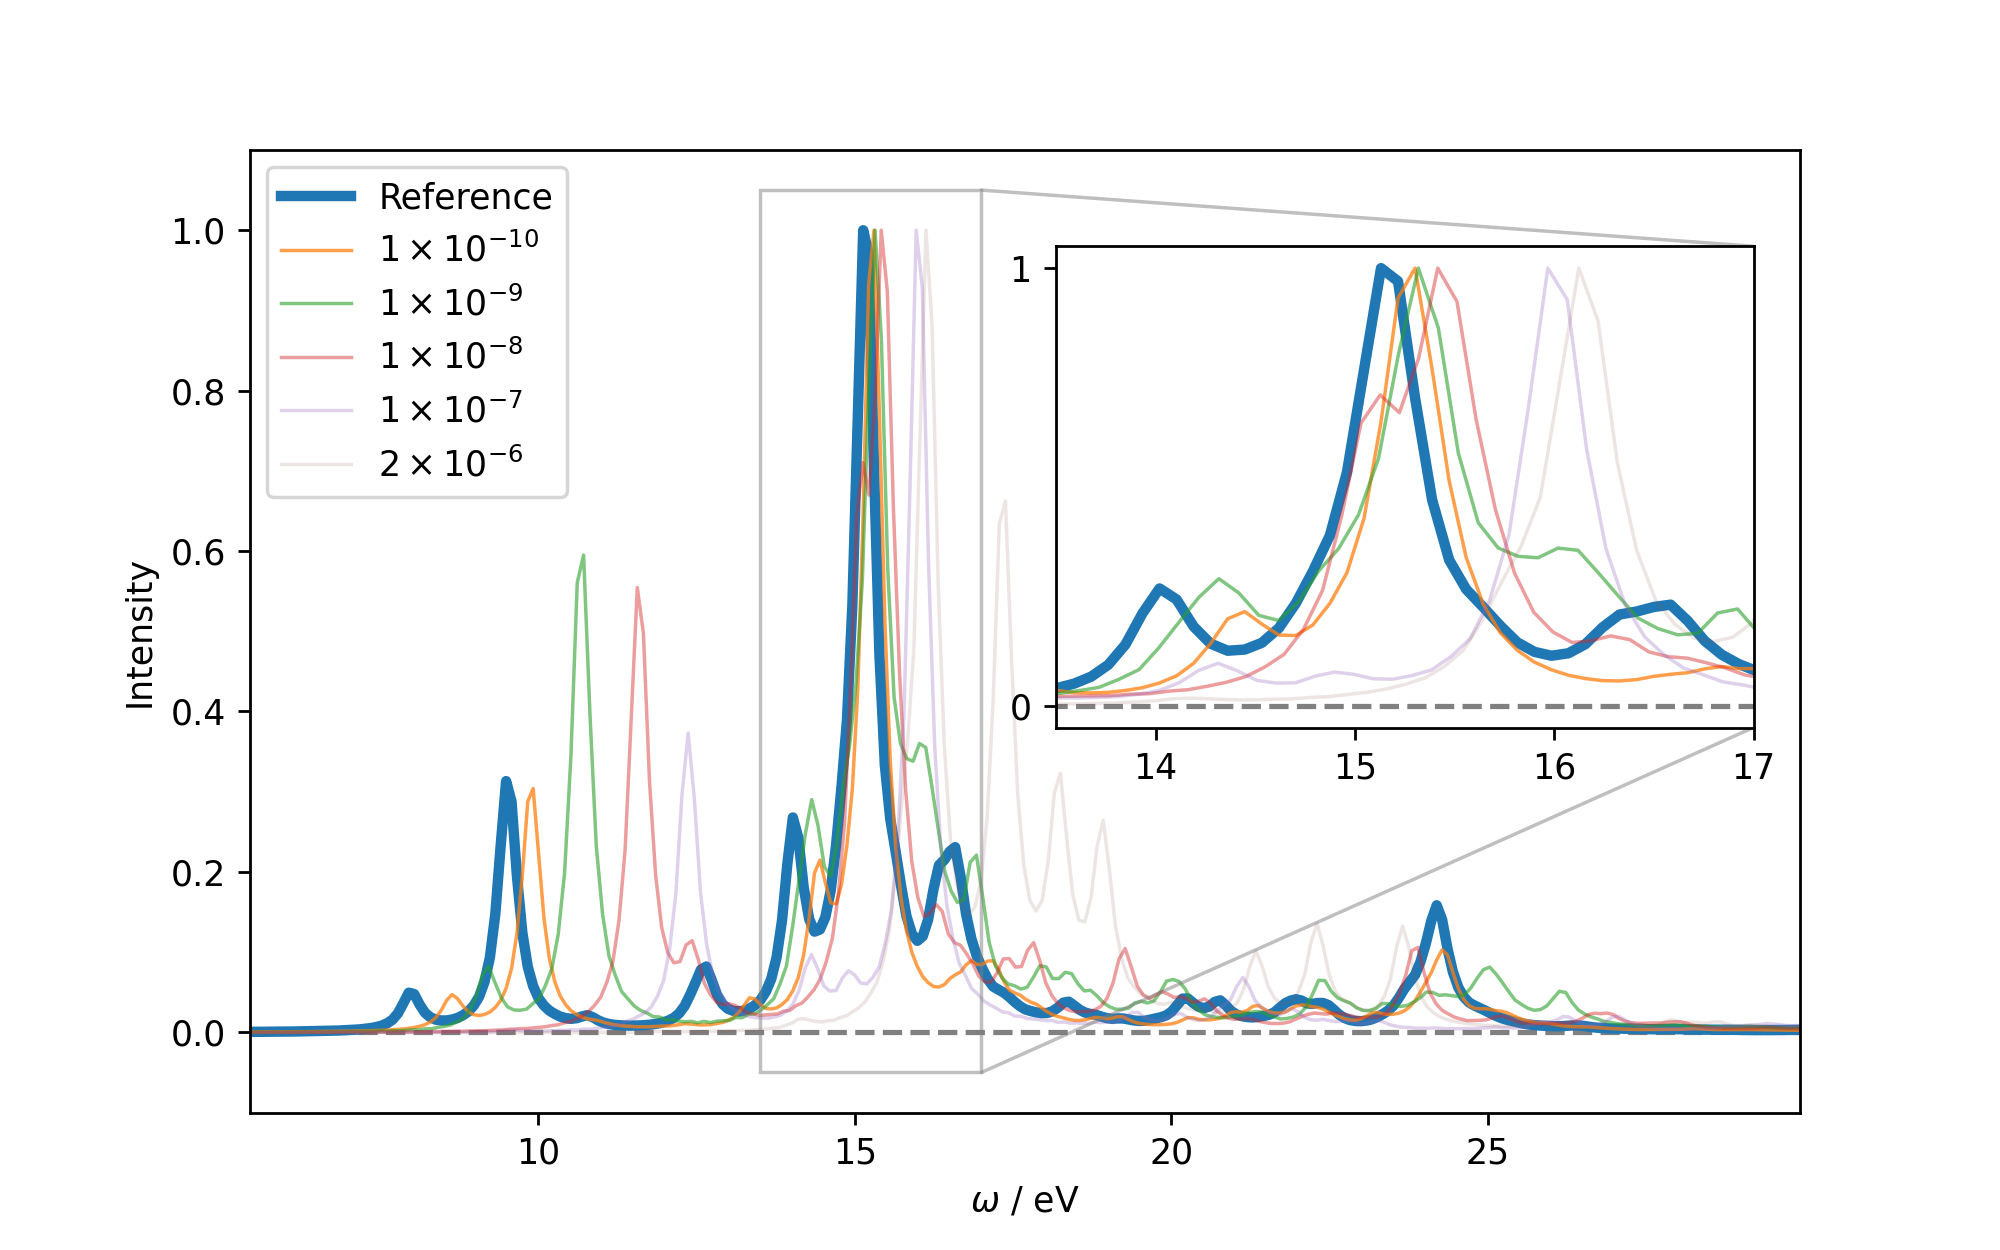
\includegraphics[scale=.6]{p3/figures/pno_abs.png}
    \caption{Reference and PNO absorption spectra for five cutoffs: 
    [$1\times 10^{-10}$, $1\times 10^{-9}$, $1\times 10^{-8}$, $1\times 10^{-7}$, 
    $2\times 10^{-6}$] corresponding to [$93\%$, $82\%$, $63\%$, $44\%$, $24\%$]
    of the MO virtual space, respectively.}
    \label{fig:pno_abs}
\end{figure}
%For all truncated PNO virtual spaces considered, the base peak appears to within 1.5 eV of the 
%reference. 
Overall, truncated PNO virtual spaces approximate the position of the base peak well,
with the smallest space predicting a base peak within 1.5 eV of the reference,
and the two largest spaces predict this peak to within 0.2 eV of the reference.
Convergence to the reference base peak occurs from the right, indicating
a lowering of excited state energies as the size of the virtual space increases. 
This trend can also be seen for the smaller peak near 10 eV. However, convergence of the shoulder 
peaks on either side of the base peak, indicated by the inset of 
Figure~\ref{fig:pno_abs}, is less predictable. Even the largest spaces considered
do not correctly predict the excitation energy, with no clear advantage to having
93\% of the virtual space as compared to just 83\% for predicting these peaks.
This trend continues into the higher-energy range of the spectrum, with the 
performance of each cutoff being nearly indistinguishable. 

Performance of the PAO space is shown in Figure~\ref{fig:pao_abs}. 
\begin{figure} 
    \centering
    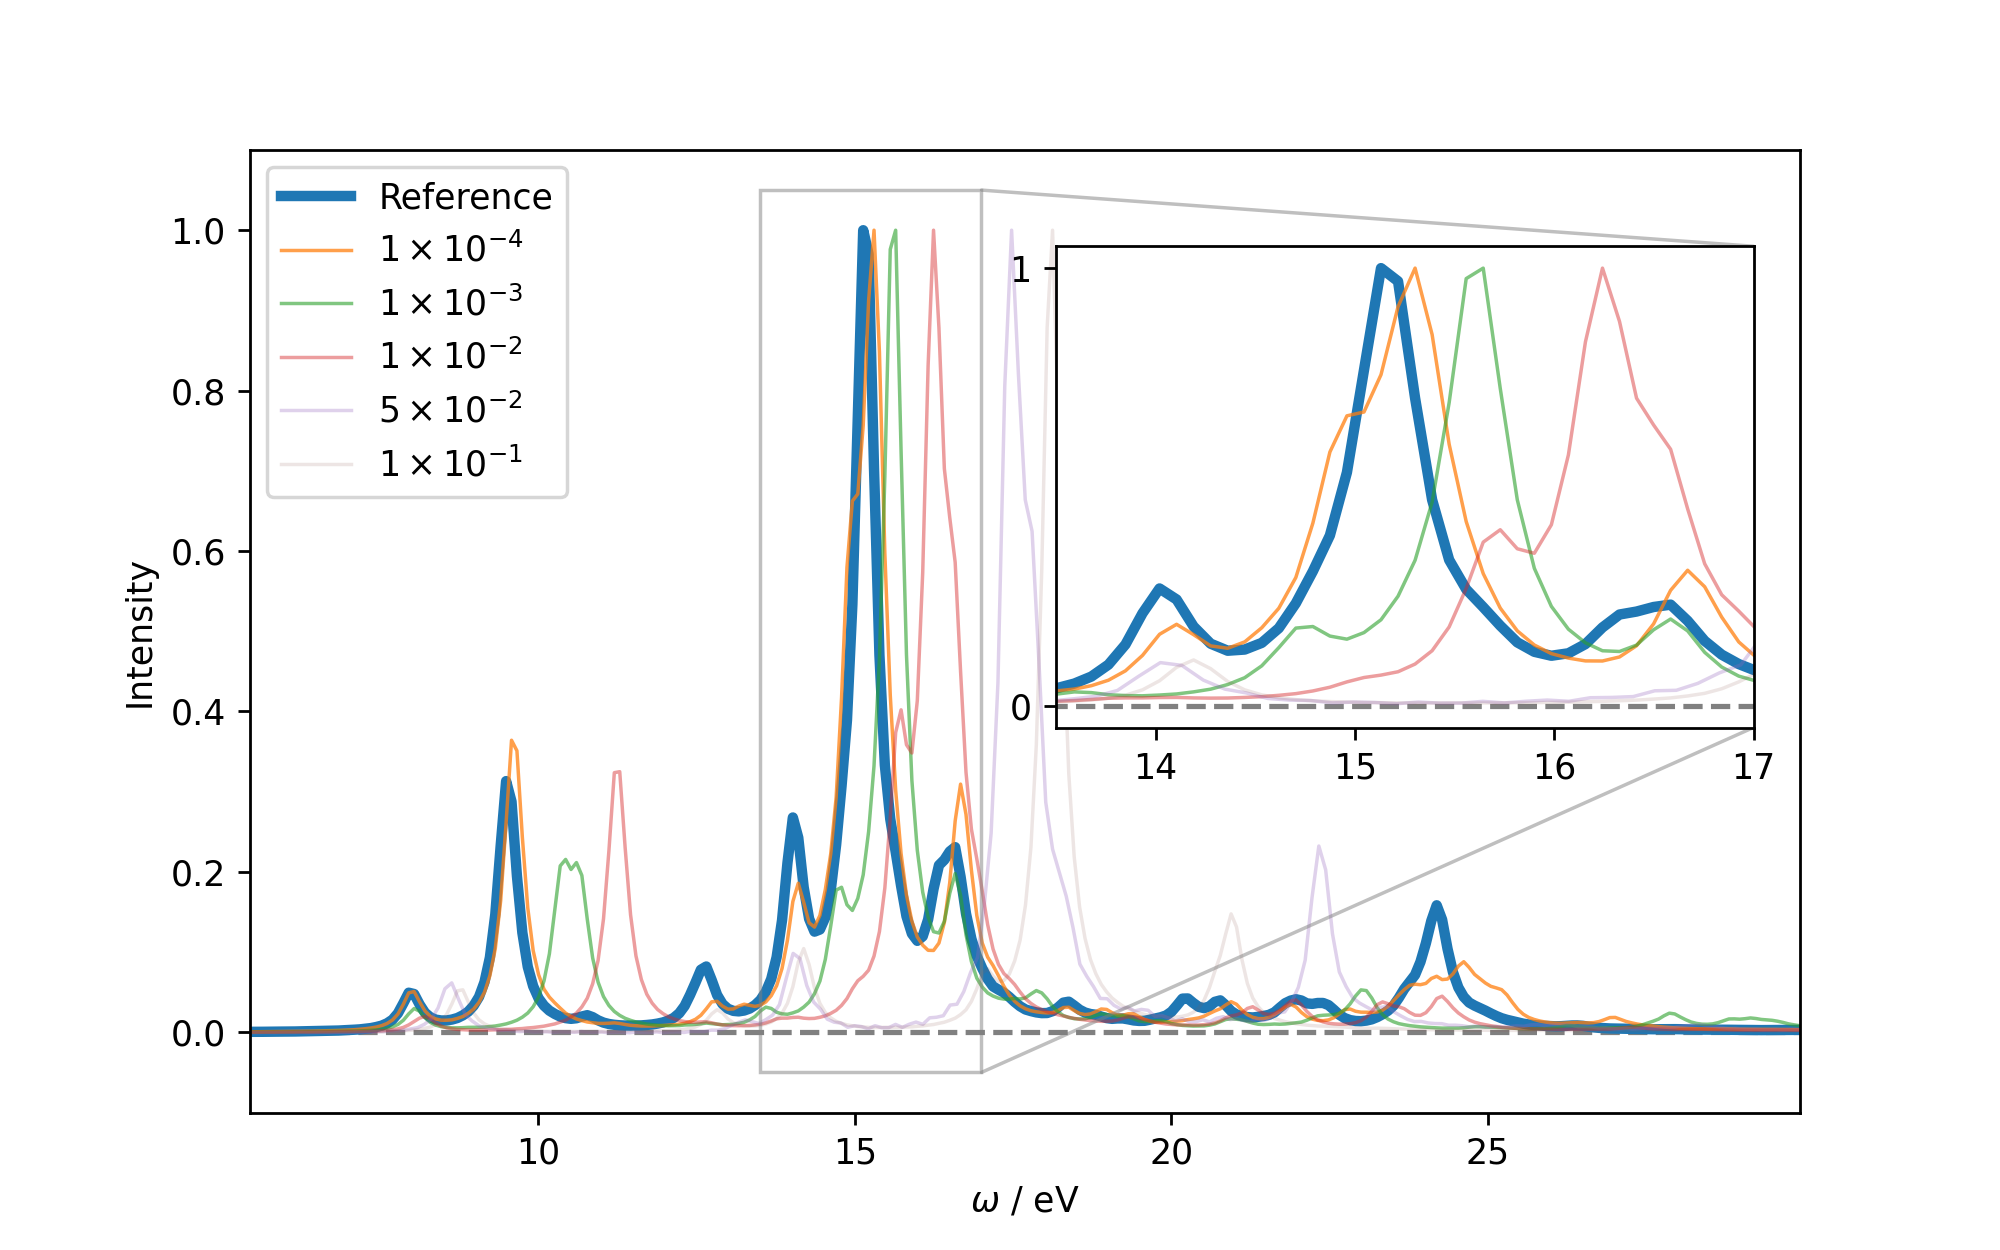
\includegraphics[scale=.6]{p3/figures/pao_abs.png}
    \caption{Reference and PAO absorption spectra for five cutoffs: 
    [$1\times 10^{-4}$, $1\times 10^{-3}$, $1\times 10^{-2}$, $5\times 10^{-2}$, 
    $1\times 10^{-6}$] corresponding to [$95\%$,$86\%$,$63\%$,$46\%$,$23\%$]
    of the MO virtual space, respectively.}
    \label{fig:pao_abs}
\end{figure}
The largest truncated PAO virtual space, on average 95\% of the MO space, accurately 
predicts the excitation energies for each major peak below 17 eV. Particularly around 10 eV, 
this is noticeably improved performance relative to the largest PNO space tested, 
with only a 2\% difference in the average size of the virtual space. 
However, accuracy rapidly declines even at 86\% of the virtual space, where the base peak
position is already worse than what was predicted with a PNO space of just 63\% of the 
MO space. Performance continues to degrade as energy increases and the average size of 
the PAO space decreases. For the final two cutoffs, at averages of 46\% and 23\% of the
MO space, the base peaks are 3 eV or more away from the reference, and no peak is 
exhibited near 25 eV. These spaces also fail to predict the second largest peak, the 
excitation just below 10 eV. 

\subsubsection{ECD} \label{sss:ecd}
Overall, neither scheme produced adequate results upon truncation of the virtual space. 
This result is not entirely surprising -- in studies of local correlation applied to 
response theory by Crawford \textit{et al}., 
\cite{McAlexander2016,Kumar2017,Crawford2019,DCunha2021} 
traditional schemes proved inaccurate for another 
electric dipole--electric dipole property, the electric polarizability.
In terms of response theory,
the polarizability (and the refractive index) is related to the \textit{real} part 
of the electric dipole--electric dipole linear response tensor 
($\boldsymbol{\alpha}_{ij}$ in Eq.~(\ref{eq:mu_exp})), 
while absorption
is related to the \textit{imaginary} part. Indeed, all linear absorptive properties
such as absorption and CD 
are related to the imaginary component of a linear response tensor, while dispersive 
properties such as refractive index and 
circular birefringence (also known as optical rotation)
are related to the real component.
\cite{Barron2004,Norman2011}
To continue, we will look at another absorptive property which is related to the mixed
electric dipole--magnetic dipole linear response tensor -- ECD.

The ECD spectrum is obtained from the Fourier transform of Eq.~(\ref{eq:ecd}).
Being a bisignate, mixed-response property, ECD is a considerable computational
challenge, similar to its dispersive counterpart circular birefringence. 
Figure~\ref{fig:pno_ecd} shows the results for an ECD spectrum in the same PNO 
orbital spaces used in the previous section.
\begin{figure} 
    \centering
    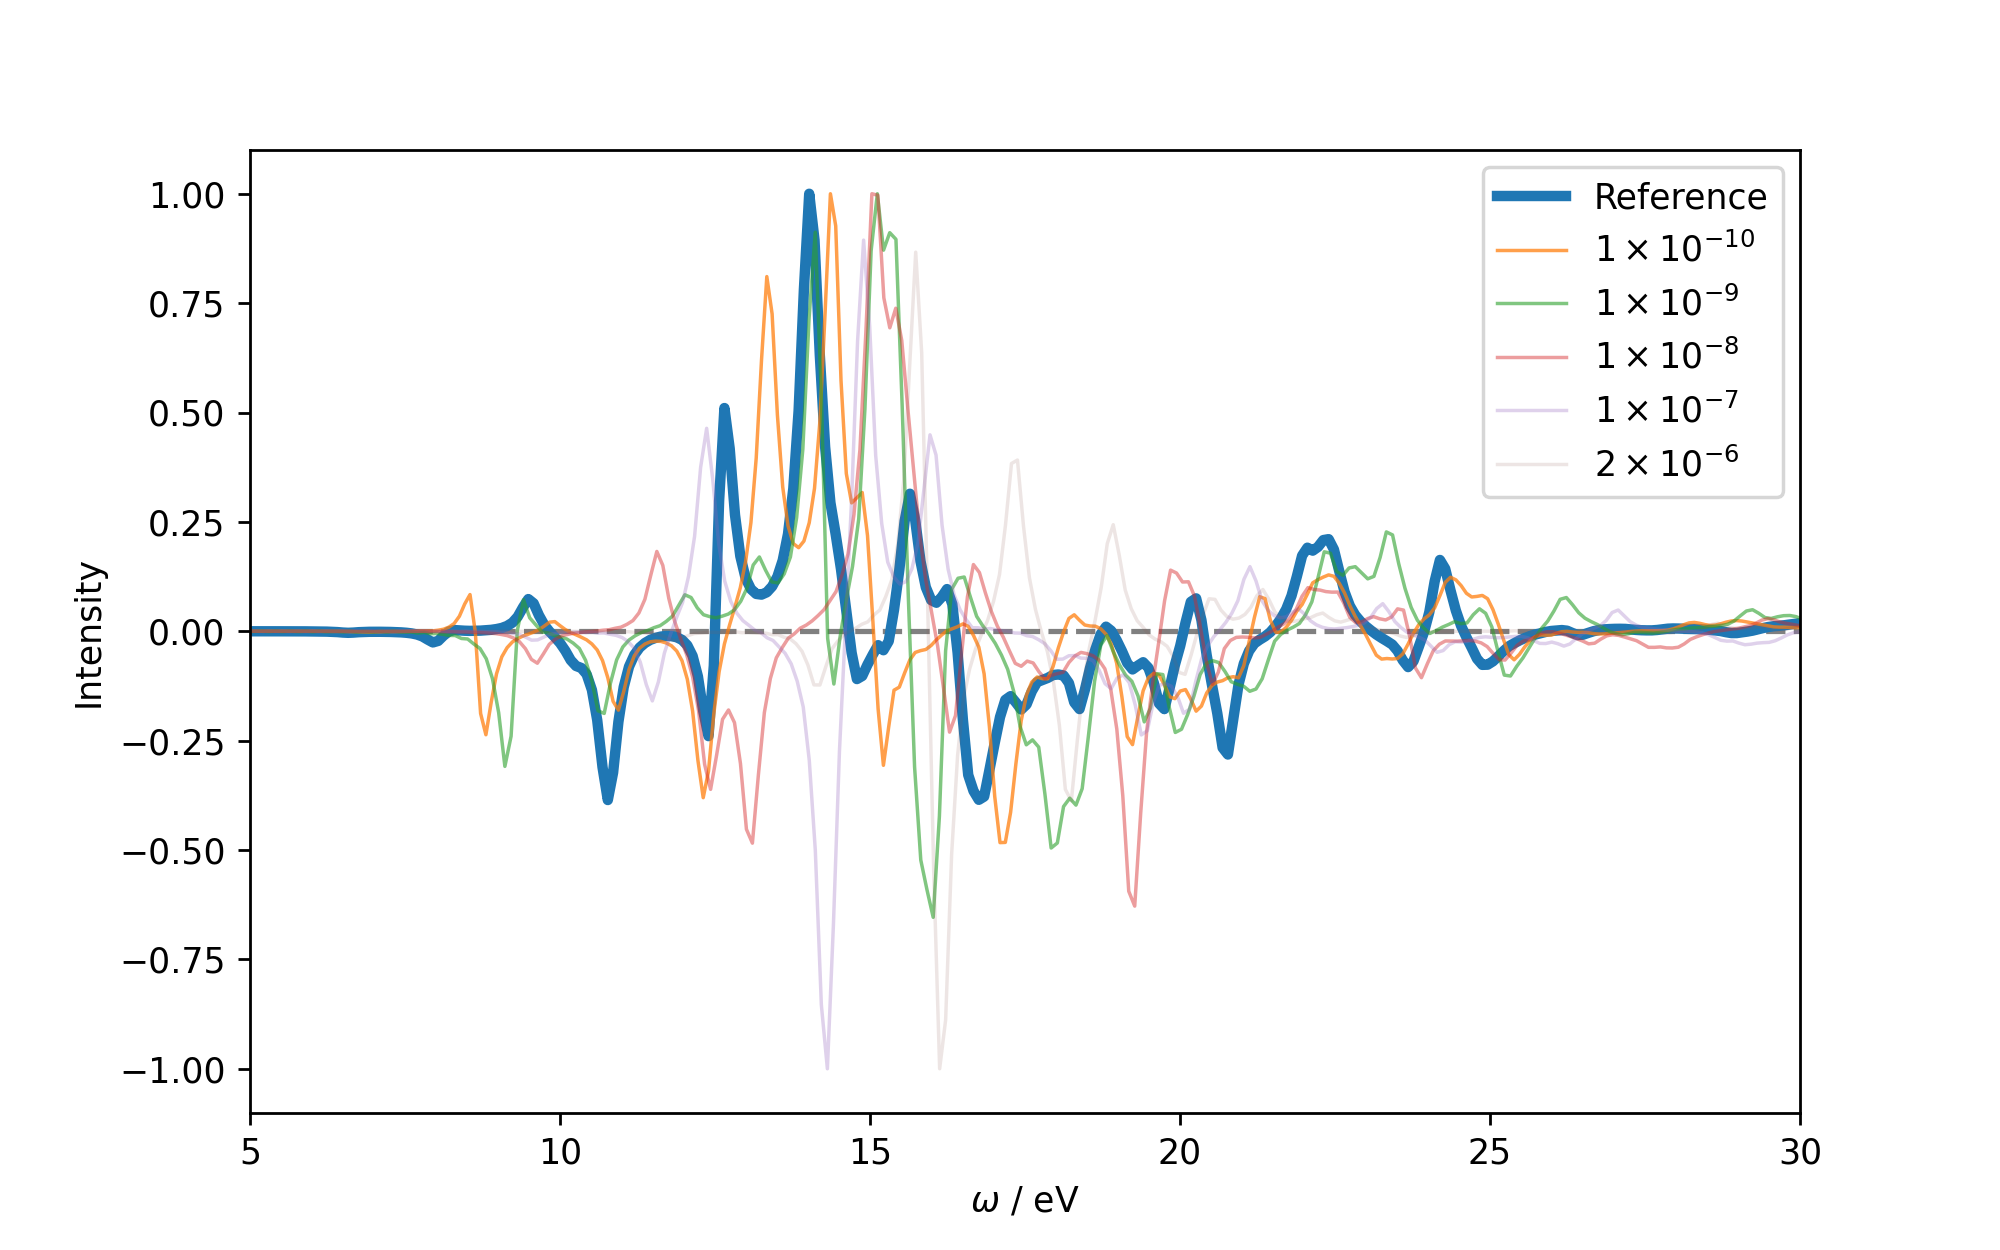
\includegraphics[scale=.6]{p3/figures/pno_ecd.png}
    \caption{Reference and PNO ECD spectra for five cutoffs: 
    [$1\times 10^{-10}$, $1\times 10^{-9}$, $1\times 10^{-8}$, $1\times 10^{-7}$, 
    $2\times 10^{-6}$] corresponding to [$93\%$,$82\%$,$63\%$,$44\%$,$24\%$]
    of the MO virtual space, respectively.}
    \label{fig:pno_ecd}
\end{figure}
The dynamic response of the magnetic dipole to the electric field in this frequency 
range is considerably more complicated than that of the electric dipole. Below 60\% of
the MO space, virtually all distinguishing characteristics of the reference 
spectrum are unidentifiable. Further, at 82\%, the base peak appears to be a pair of 
peaks, more resembling the pair of peaks appearing just above 15 eV in the 
reference spectrum, with the major peak just below 15 eV being the second strongest.
At an average of 93\%, the overall \textit{shape} of the spectrum in the 10 eV to 
20 eV range more closely resembles that of the reference; however, the excitation
energies are, in some cases, even less accurate than those of smaller PNO spaces.
The trend of lowering excited state energies with increased virtual space seen in 
Section~\ref{sss:ecd} is no longer discernible. 

As in the case of absorption, the PAO basis is not noticeably more efficient at
approximating the full MO space than the PNO space. Figure~\ref{fig:pao_ecd} 
shows the results using the same truncated PAO spaces as in Section~$\ref{sss:abs}$.
\begin{figure} 
    \centering
    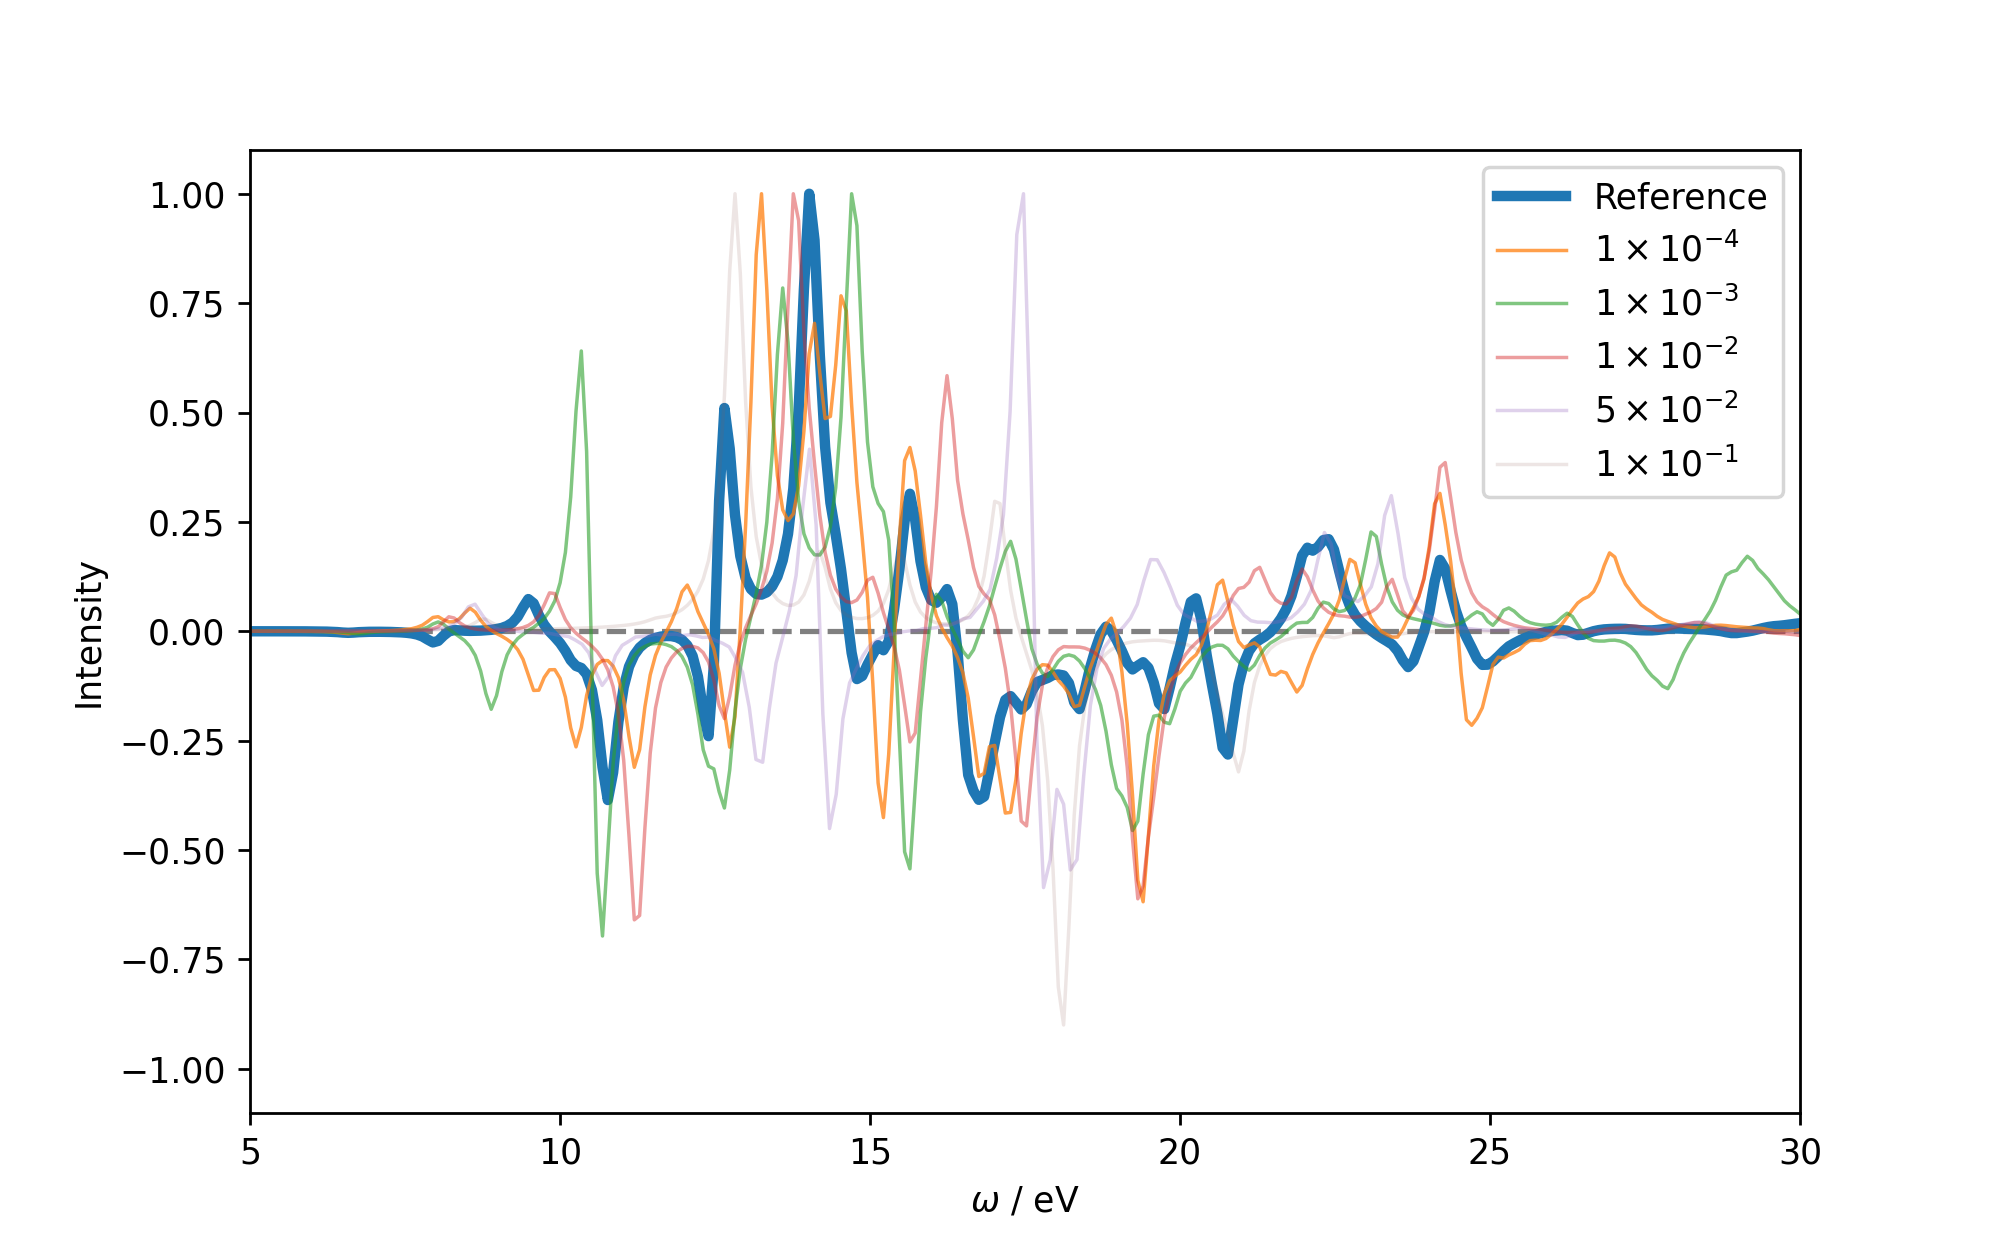
\includegraphics[scale=.6]{p3/figures/pao_ecd.png}
    \caption{Reference and PAO ECD spectra for five cutoffs: 
    [$1\times 10^{-4}$, $1\times 10^{-3}$, $1\times 10^{-2}$, $5\times 10^{-2}$, 
    $1\times 10^{-6}$] corresponding to [$95\%$,$86\%$,$63\%$,$46\%$,$23\%$]
    of the MO virtual space, respectively.}
    \label{fig:pao_ecd}
\end{figure}
The performance of the PAO basis near the base peak varies wildly with truncation,
as in the PNO case. In the low-frequency region, the PAO results are considerably 
worse -- see the two negative peaks between 10 eV and 15 eV. Curiously, the 
largest PAO spaces considered predict significant peaks above 25 eV that are not 
present in the reference, any of the PNO spaces tested, or the smaller PAO
spaces. This suggests a strong sensitivity of the response of the wave function
to the completeness threshold used for determining the occupied domains.
%fundamentally different electronic structure in the
%presence of the perturbing field, which is a direct result of the charge-based 
%completeness threshold used for determining the occupied domains.
%albeit at very large frequencies which are of little practical use.

\subsection{Amplitude Dynamics} \label{ss:amps}
As evidenced by the preceding data, the truncated PNO and PAO virtual spaces do not
efficiently model the wave function in the presence of a perturbing EMF. As noted in
Section~\ref{sss:abs}, these shortcomings are well-documented in the case of response
theory. However, a real-time formalism offers the opportunity to analyze the wave 
function in great detail over time, perhaps shedding light on \textit{where} and 
\textit{how} the locally correlated wave functions are deficient. The following
section will scrutinize the $t_\mu$ and $\lambda_\mu$ amplitudes of 
Eqs.~(\ref{eq:t_mu}) and (\ref{eq:l_mu}), respectively, in hopes of determining the 
important fluctuations in the wave function and whether these spaces sufficiently 
capture these changes.

Response to external perturbations by the CC amplitudes give rise to
dynamic energetics and properties. In the past, distributions of perturbed amplitudes
(relative to their ground-state counterparts) have been used to justify the 
difficulty in computing response functions with local correlation methods in the 
frequency domain. 
\cite{McAlexander2016,Crawford2019,DCunha2021} 
However, initial findings show that in RTCC, the relative distribution of amplitudes 
by magnitude is not significantly impacted.\cite{Crawford2019} 
Despite this, typical means of exploiting amplitude
sparsity have been shown to be inefficient by the preceding sections. 
First, to understand the response of 
the amplitudes to the external perturbation, we plot the 
change in the norm of the amplitude tensors relative to the ground-state amplitudes 
as a function of time in Figure~\ref{fig:norm}.
\begin{figure} 
    \centering
    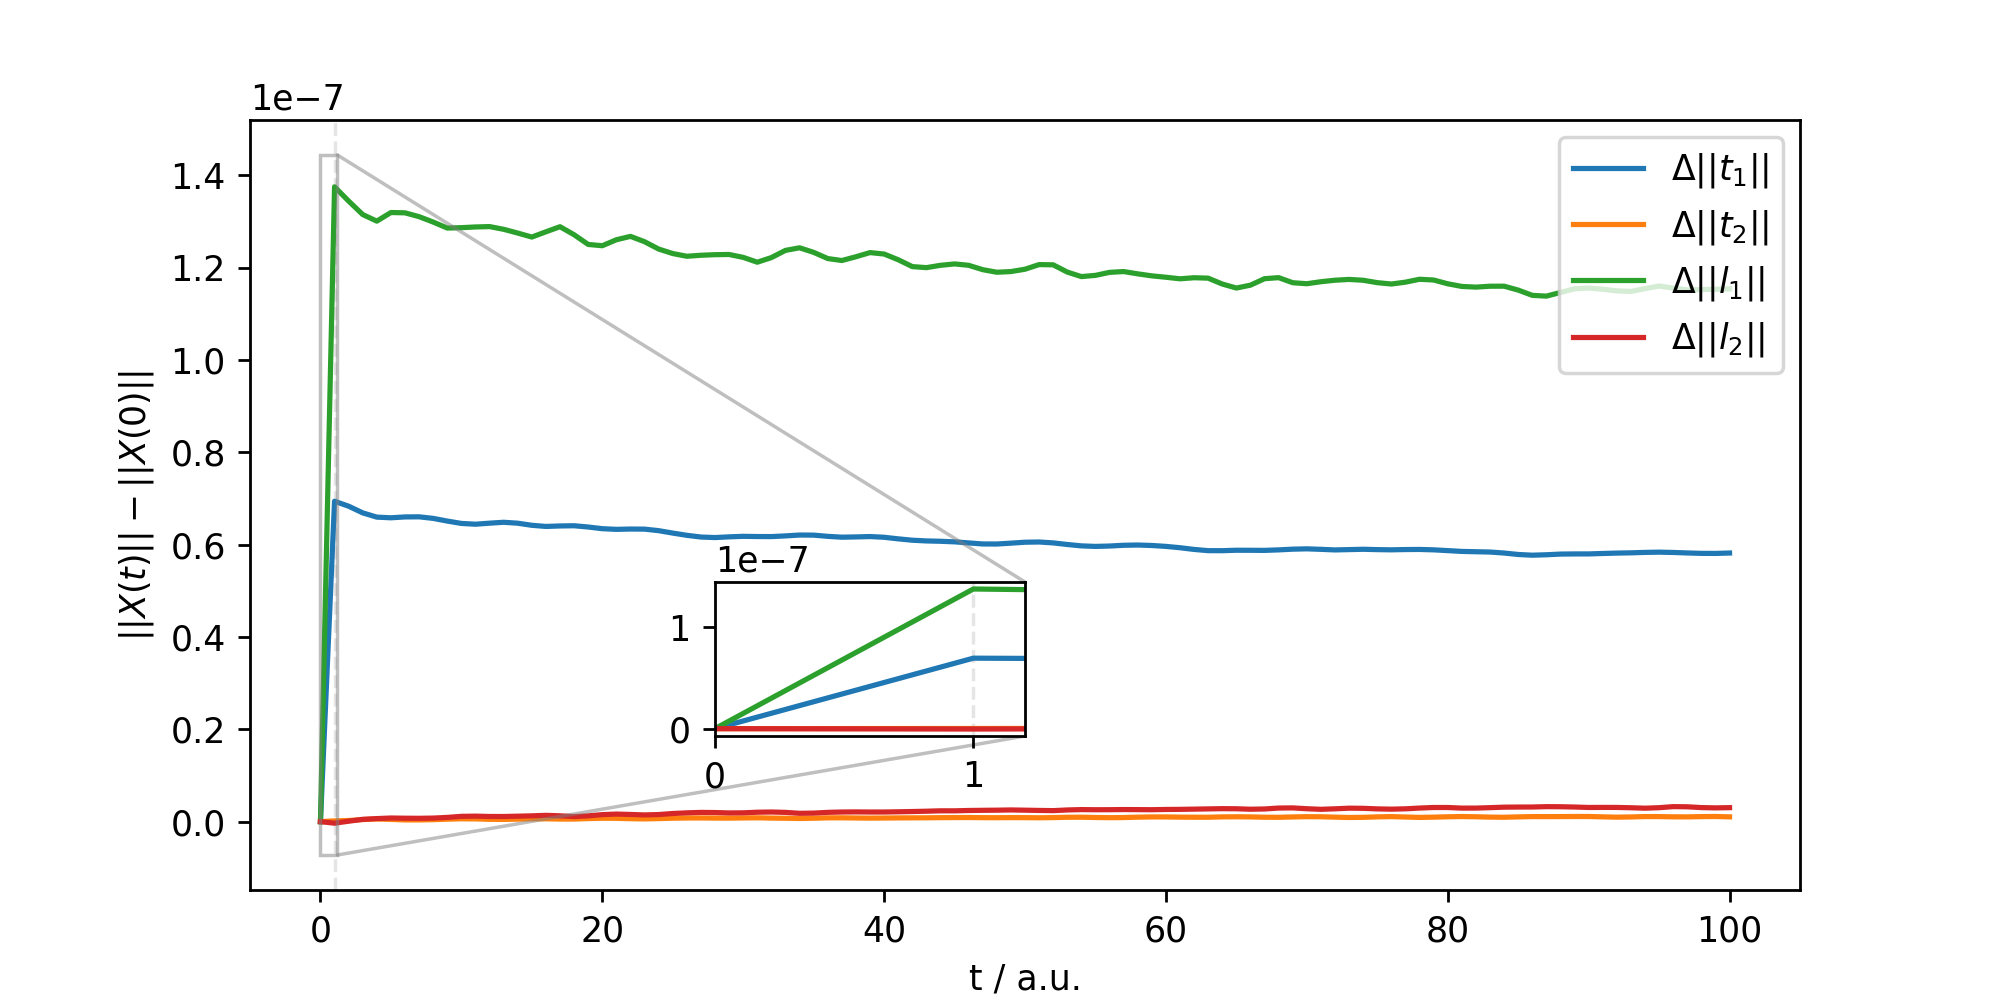
\includegraphics[scale=.6]{p3/figures/amp_norm.png}
    \caption{Time-dependent change in the norm of the amplitude 
    tensors relative to the ground-state amplitudes.
    (Field and step parameters remain unchanged, and 
    the amplitude norm is taken at every 1 a.u.)}
    \label{fig:norm}
\end{figure}
Results for the untruncated PNO and PAO spaces are identical to those
for the MO space, as the unitary transformations resulting from untruncated localized virtual spaces
in Eqs.~(\ref{eq:rotate}) preserves the tensor norm.
Amplitude norms from propagations carried out in truncated PNO and PAO spaces
are nearly indistinguishable (see SI).

Figure~\ref{fig:norm} shows that the magnitude of the response by the wave function
is predominantly within the singles amplitudes $t_1$ and $\lambda_1$. This is 
consistent with the notion that singles are paramount for the computation of 
response properties.\cite{Christiansen1995,Koch1997} However, the form of Eq.~(\ref{eq:pair_D})
does not include any contributions by singles, due to being built from MP2-level
amplitudes where singles do not contribute until at least the second order 
in the wave function and fourth order in the energy. This suggests that even in schemes
which seek to include the EMF perturbation in the construction of the reduced virtual space,
such as PNO++,\cite{DCunha2021} response of the singles should be considered.

Aside from the matrix norm, we can also inspect the individual amplitudes to track
their evolution in time. The heat maps in Figure~\ref{fig:amps} show the difference 
in $t_1$ amplitudes, relative to the ground state, for three time steps selected 
from the first 100 a.u. of the simulation.
\begin{figure}
    \begin{subfigure}{.5\textwidth}
        \centering
        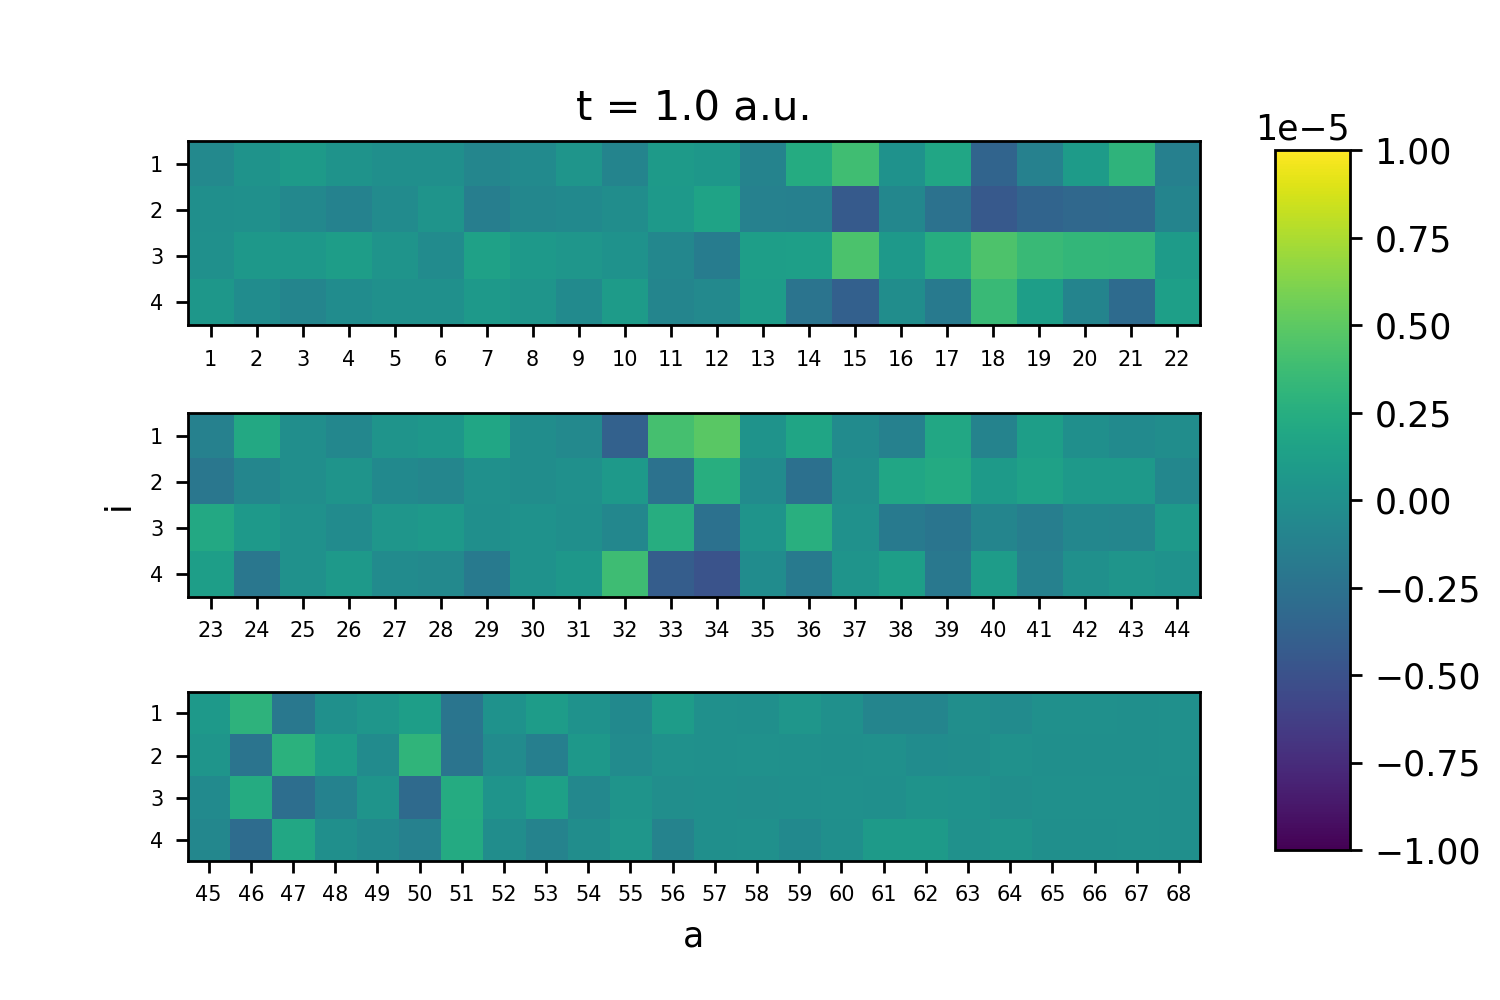
\includegraphics[scale=0.5]{p3/figures/MO_delta_t1_1.png}
        \caption{}
        \label{fig:MO_t1_1}
    \end{subfigure}%
    \begin{subfigure}{.5\textwidth}
        \centering
        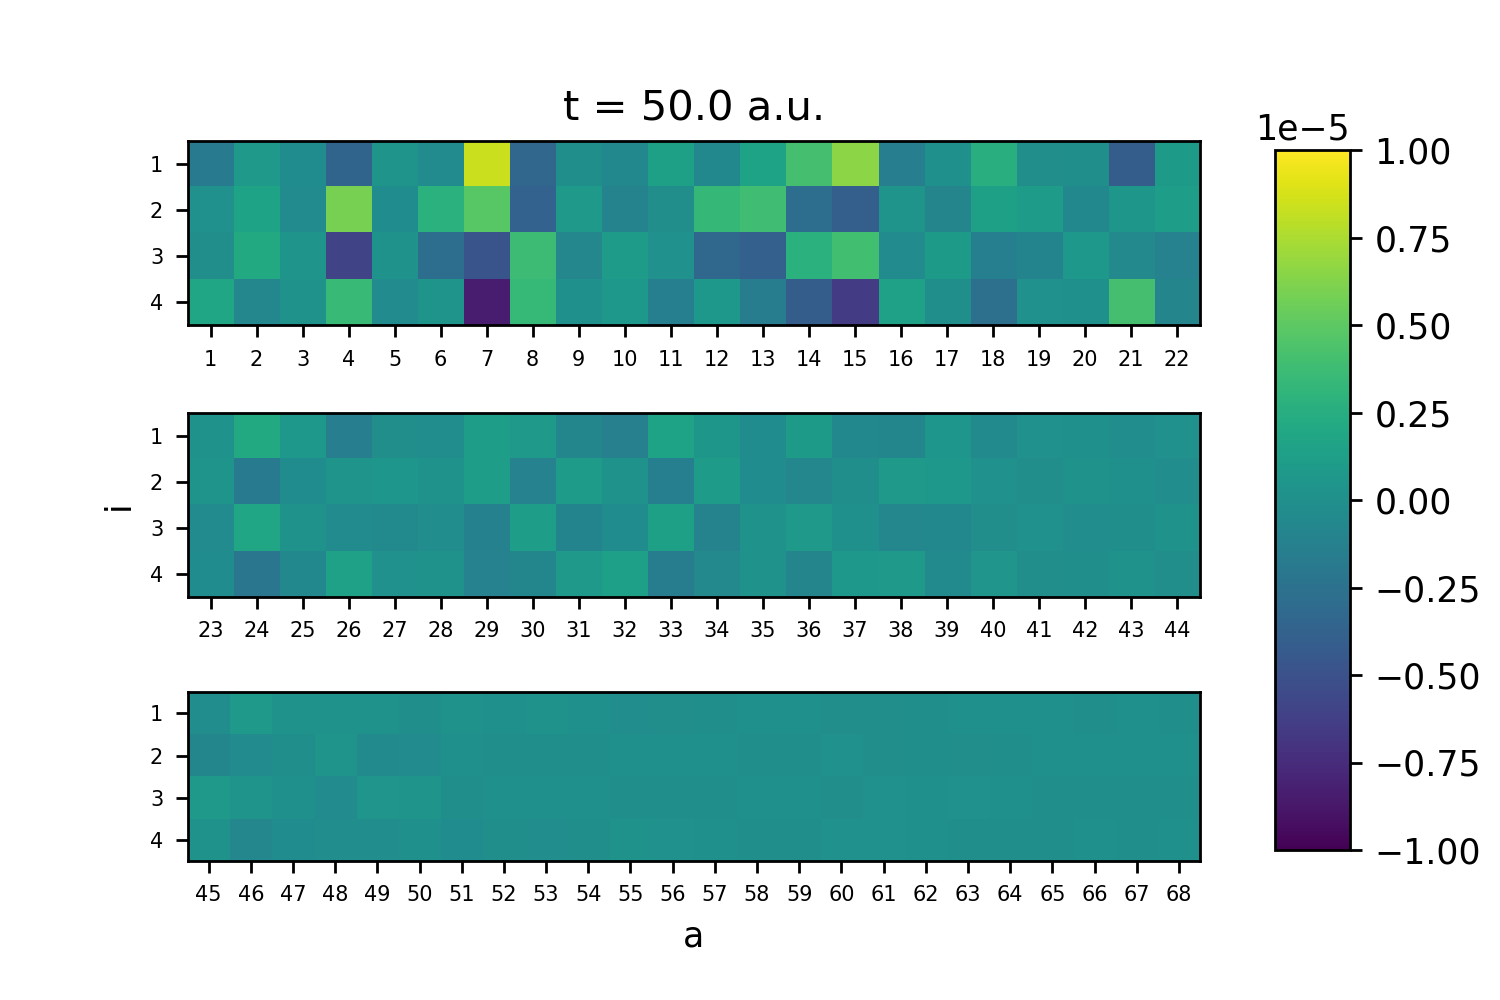
\includegraphics[scale=0.5]{p3/figures/MO_delta_t1_50.png}
        \caption{}
        \label{fig:MO_t1_50}
    \end{subfigure}
    \begin{subfigure}{.5\textwidth}
        \centering
        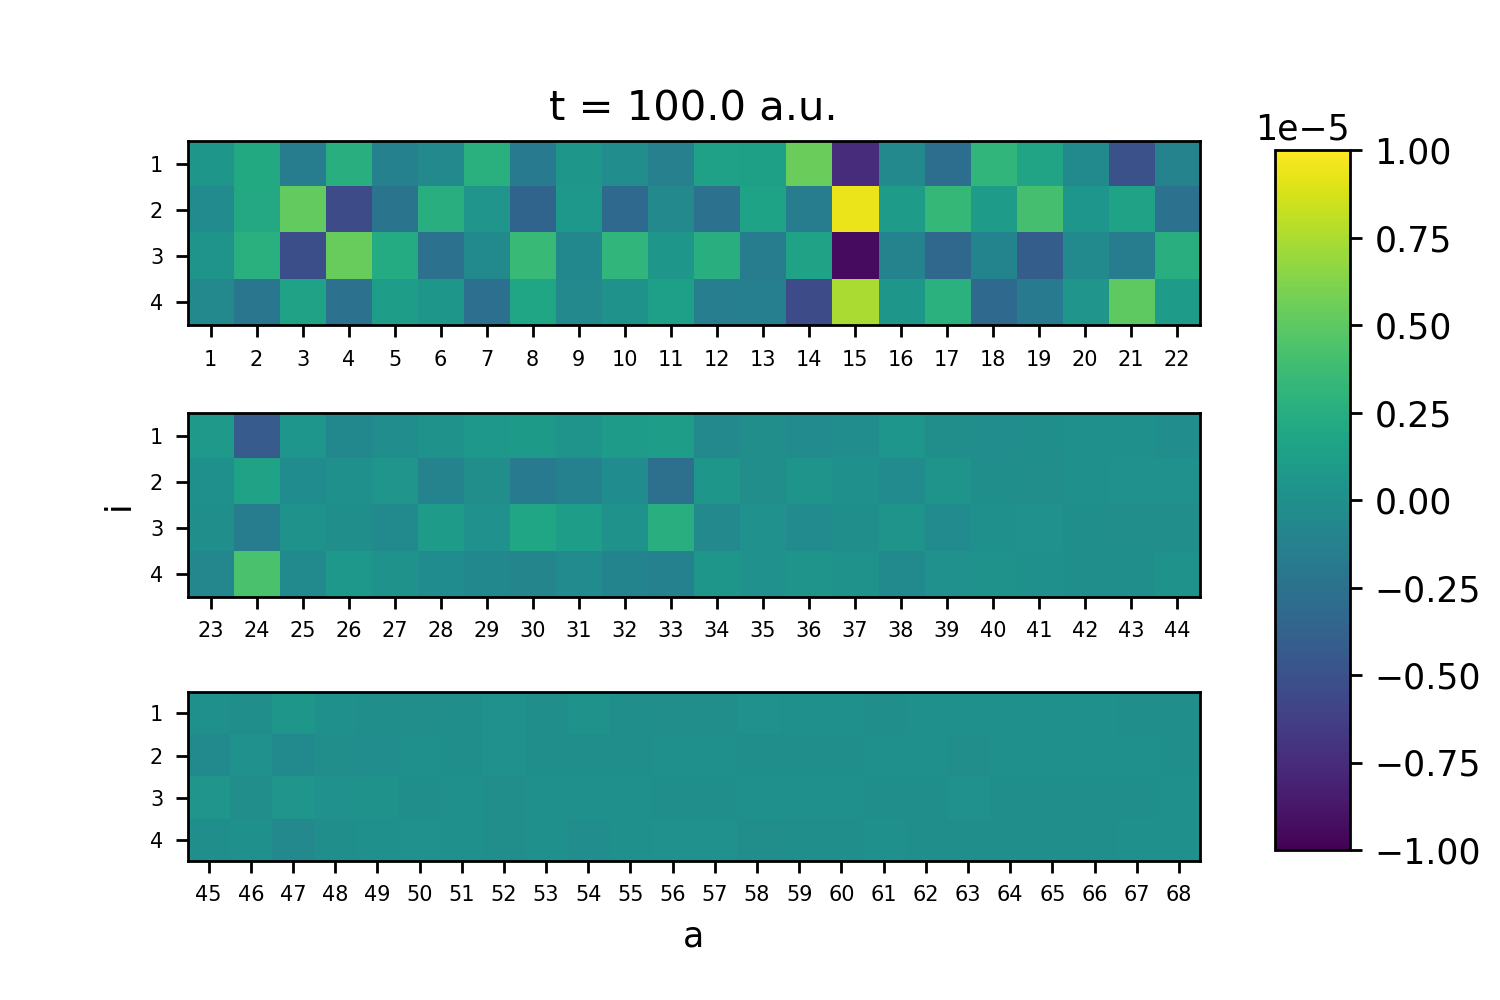
\includegraphics[scale=0.5]{p3/figures/MO_delta_t1_100.png}
        \caption{}
        \label{fig:MO_t1_100}
    \end{subfigure}
    \caption{MO-basis $t_1$ amplitude deviations from $t = 0$ after (a) 1 a.u., (b) 50 a.u., and 
    (c) 100 a.u. of time propagation. Each row contains the same four occupied orbital indices
    and a subset of virtual indices as indicated by the x-axis labels.}
    \label{fig:amps}
\end{figure}
The amplitudes are ordered by the orbital energies of the associated MOs. 
The amplitudes which experience significant oscillations vary throughout the simulation,
though there are several discernible trends. First, most large amplitude deviations
are associated with all occupied orbitals simultaneously. This is due to the relatively small size of 
the system, with only four occupied orbitals, all of which are likely important in the
description of the ground- and excited-state wave functions. Secondly, 
at any given time during the propagation,
a large number of amplitudes have not significantly deviated from their ground state values.
This supports the notion
that relative sparsity is maintained within the amplitudes throughout the simulation,
but this sparsity is distributed differently throughout the amplitude tensors as
the wave function is propagated.  

A third trend is that amplitudes which respond strongly tend to be associated with 
low-energy virtual orbitals. Chemical intuition would suggest that energetically 
low-lying molecular orbitals will be the most involved in electronic excitations.
However, while amplitude responses are indeed larger for lower-energy virtual orbitals, 
smaller amplitude 
deviations in Figure~\ref{fig:amps} extend far into the virtual space. This explains
the difficulty of simply truncating with respect to orbital energy: the 
high-energy MOs are still important to the time-evolution of the wave function 
in the presence of an EMF. 

Figure~\ref{fig:pno_amps} shows the $t_1$ amplitudes for the same simulation,
rotated into the untruncated PNO basis using $Q_{ii}$ as defined in
Eq.~(\ref{eq:Q_pno}).
\begin{figure}
    \begin{subfigure}{.5\textwidth}
        \centering
        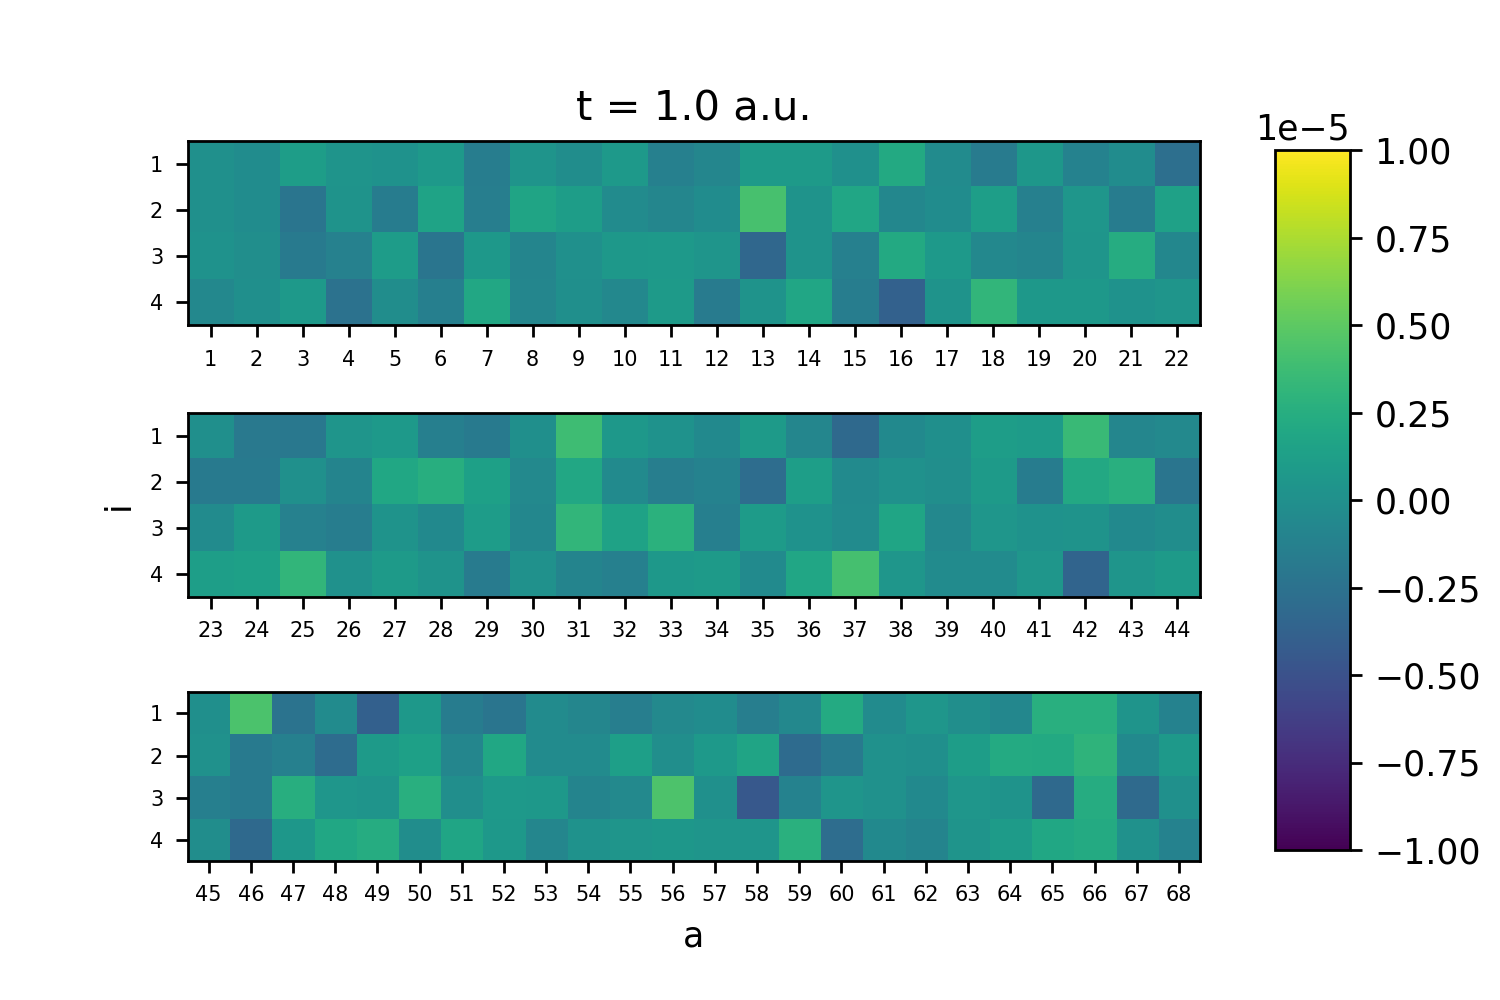
\includegraphics[scale=0.5]{p3/figures/PNO_delta_t1_1.png}
        \caption{}
        \label{fig:PNO_t1_1}
    \end{subfigure}%
    \begin{subfigure}{.5\textwidth}
        \centering
        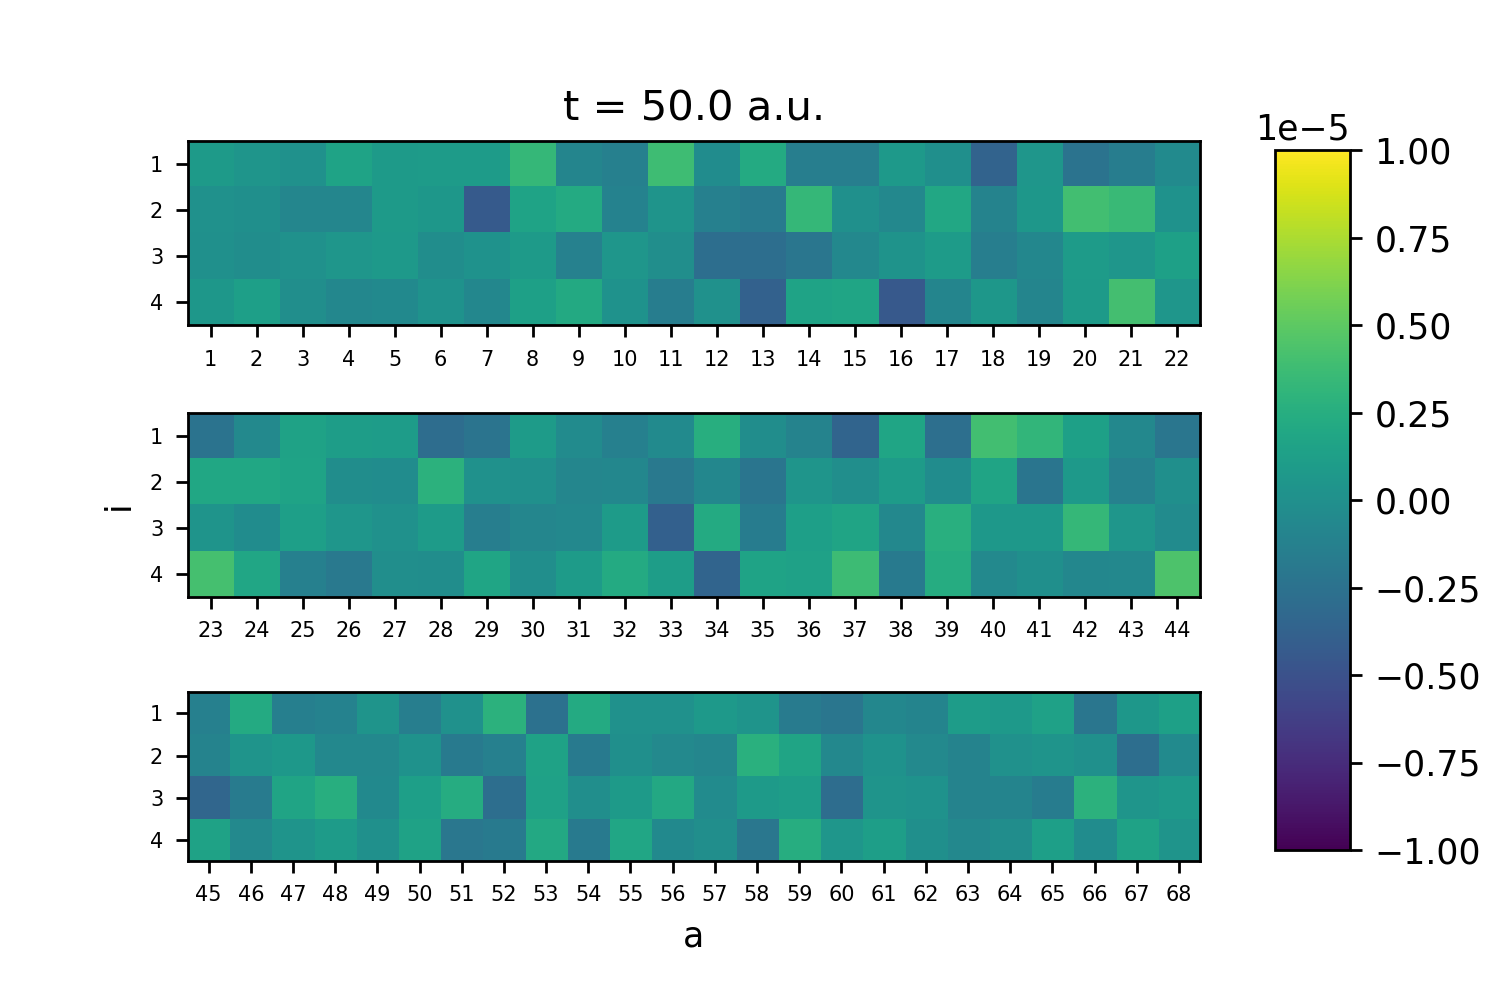
\includegraphics[scale=0.5]{p3/figures/PNO_delta_t1_50.png}
        \caption{}
        \label{fig:PNO_t1_50}
    \end{subfigure}
    \begin{subfigure}{.5\textwidth}
        \centering
        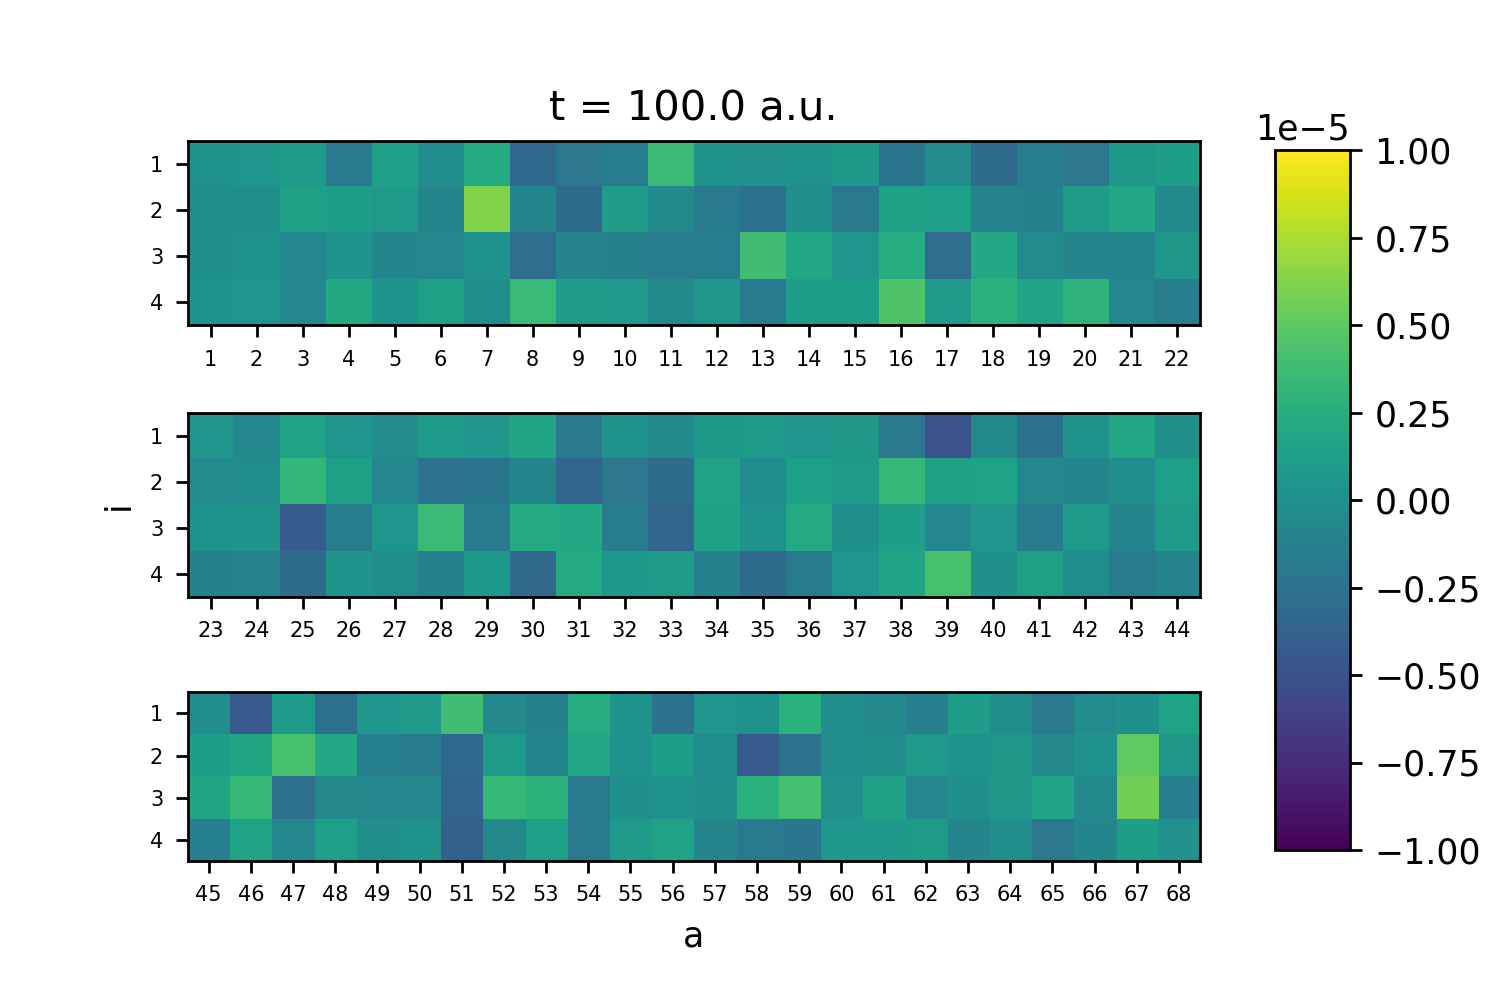
\includegraphics[scale=0.5]{p3/figures/PNO_delta_t1_100.png}
        \caption{}
        \label{fig:PNO_t1_100}
    \end{subfigure}
    \caption{PNO-basis $t_1$ amplitude deviations from $t = 0$ after (a) 1 a.u., (b) 50 a.u., and 
    (c) 100 a.u. of time propagation. Each row contains the same four occupied orbital indices
    and a subset of virtual indices as indicated by the x-axis labels.}
    \label{fig:pno_amps}
\end{figure}
(It should be noted that, due to redundancy in the AO-based virtual 
spaces for each pair, PAO-basis amplitudes cannot be compared directly in 
this manner.)
It can be immediately seen that the amplitude deviations
are less sparse in the PNO basis after the application of the EMF. 
Many more amplitudes exhibit
perceivable differences, and strong deviations (magnitudes approaching 
$1\times 10^{-5}$) are no longer present. This is a clear demonstration
of the issue with truncating orbital spaces based on the present criterion ---
rather than exploiting sparsity, the amplitude tensors have become less sparse.
It may also suggest a recipe for building a more appropriate 
virtual space for truncation. 
In the following section, we propose some alternative schemes based on the 
literature and the results of this study.
%In the following section, we compare a selection
%of orbitals which correspond to strong amplitude deviations in the MO basis 
%(specifically virtuals 3, 4, 7, and 15)
%based on orbital spatial extent to determine if this may be a possible criterion 
%for truncation of the virtual space.

\subsection{Possible Alternatives} \label{ss:alt}
\begin{figure}
    \centering
    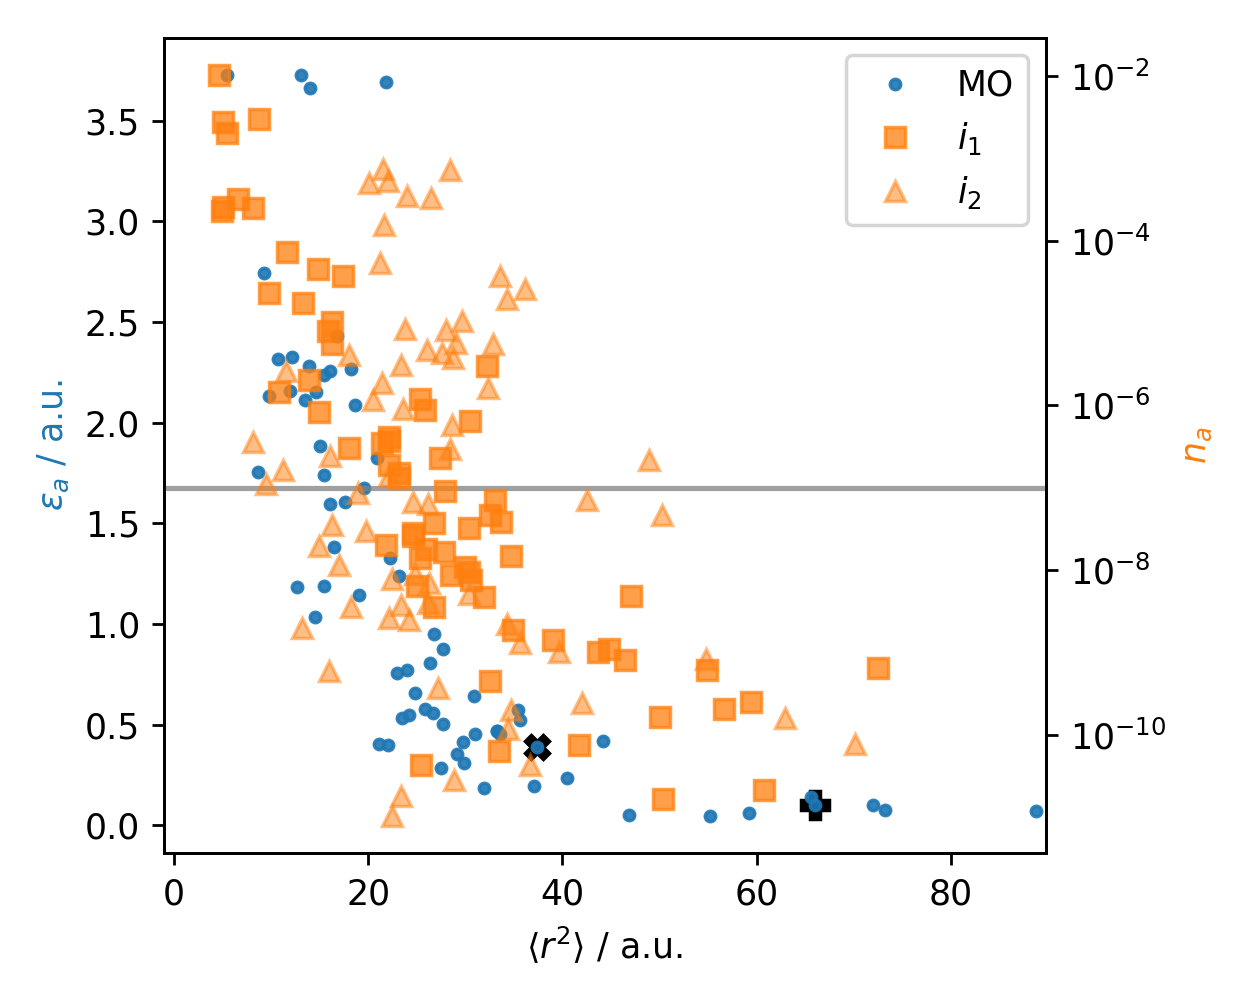
\includegraphics[scale=0.75]{p3/figures/extent.png}
    \caption{Virtual MO energy $\epsilon_a$ and the
    occupation number $n_a$ (plotted on a log scale)
    for unique PNO spaces $i_1$ and $i_2$ 
    versus orbital extent in arbitrary units.
    Virtual MOs 7 and 15 are denoted by a solid $\boldsymbol{+}$ 
    and $\boldsymbol{\times}$, respectively.
    The horizontal line denotes a PNO cutoff 
    of $1\times 10^{-7}$.}
    \label{fig:extent}
\end{figure}
Figure~\ref{fig:extent} shows the virtual MO energy $\epsilon_a$ and the 
PNO occupation number $n_a$ plotted against the orbital extent
$\langle r^2 \rangle$ in arbitrary units. 
In the PNO basis, a unique virtual space is prepared
for every occupied pair, resulting in 16 unique spaces for the four occupied
spatial orbitals $i$. However, for transforming
a single orbital index, we only require the diagonal rotation matrices,
\textit{i.e.}, $Q_{ii}$. There are four such spaces; however, by symmetry,
only two are unique. Both are included in Figure~\ref{fig:extent}. 

Truncation of the PNO space begins from the bottom of Figure~\ref{fig:extent}. 
At an occupation number cutoff of $1\times 10^{-7}$ (indicated by a horizontal
line), all orbitals below this line are neglected in the PNO space. Roughly
66\% of the virtual space lies in this region. From these data, it is clear
that even modest truncation of the virtual space neglects the diffuse 
regions of the wave function, which are important for excited-state
properties in systems with significantly delocalized characteristics,
such as systems containing Rydberg-type excitations.

%Table~\ref{ta:ext} reports the orbital extent $\langle r\rangle$ for virtual orbitals $a$
%corresponding to four of the strongest deviations in Figure~\ref{fig:amps}. 
%These orbitals are labeled 4, 7, 8, and 15, in
%both the MO and PNO basis. In the PNO basis, a unique virtual space is prepared
%for every occupied pair, resulting in 16 unique spaces for the four occupied
%spatial orbitals $i$. However, for transforming
%a single orbital index, we only require the diagonal rotation matrices,
%\textit{i.e.}, $Q_{ii}$. There are four such spaces; however, by symmetry, the domains of occupied
%orbitals 1 and 4 are the same, as are 2 and 3. Thus, orbital extents for only those
%two unique orbital spaces $i_1$ and $i_2$  are shown.
%\begin{table}
%    \centering
%    \begin{tabular}{|c|c|c|c|}
%        \hline
%%        $a$ &   MO  &   PNO   &        \\  
%        $a$ &  MO  &   \multicolumn{2}{c|}{PNO} \\  
%        \hline
%%        \multicolumn{2}{|c|}{}  & $i_1$   & $i_2$  \\ 
%            &       & $i_1$   & $i_2$  \\
%        \hline
%%         3  & 59.23 & 7.9     & -24.67 \\ 
%%        \hline
%         4  & 88.76 & -13.08  & -3.13  \\ 
%        \hline
%         7  & 66.00 & 0.73    & -0.07  \\ 
%        \hline
%         8  & 65.56 & -3.91   & -10.35 \\ 
%        \hline
%         15 & 37.39 & -15.11  &  1.32  \\
%        \hline
%    \end{tabular}
%    \caption{Orbital spatial extent of four selected virtual orbitals in the MO
%    and PNO spaces.}
%    \label{ta:ext}
%\end{table}
%A full table of virtual orbital extents can be found in the SI. 
%In the MO basis, the orbitals in Table~\ref{ta:ext} 
%correspond to the strongest amplitude deviations in Figure~\ref{fig:amps}.
%These are also some of the most diffuse orbitals in this basis,
%far larger than the average orbital extent of 26.62.
%As expected, the spatial extent of the PNOs built upon the MOs
%are much more localized. This shows that, in the MO basis,
%strong deviations are predominantly exhibited by amplitudes 
%corresponding to virtual orbitals with a larger spatial extent,
%creating sparsity. In the PNO basis, however, the deviations 
%are evenly spread across a large number of amplitudes corresponding
%to orbitals with relatively small spatial extent, resulting in 
%less sparsity in the amplitude tensor. 
%These findings suggest that virtual domains built for excited state
%properties should seek to include orbitals with large spatial extent,
%and any truncation criterion should preserve these orbitals.

Spatial extent alone may not be a suitable criterion for truncation -- 
this would have obvious a negative impact on the accuracy of the 
correlation energy, which is inherently local in nature. 
Additionally, Figure~\ref{fig:extent} highlights virtual MOs 7 
($\boldsymbol{+}$) and 15 ($\boldsymbol{\times}$),
which correspond to the strongest deviations in 
Figures~\ref{fig:MO_t1_50} and \ref{fig:MO_t1_100}, respectively.
That these orbitals are of varying extent
demonstrates that both diffuse and contracted orbitals play a role in 
the wave function dynamics.
In order to attain a balanced description of wave function components 
important for both energy and property calculations, the combination 
of appropriately determined spaces such as the combined PNO++ approach
has been fruitful. Still neglected in this approach
are the singles amplitudes, which are absent in the MP2 wave functions
used to approximate the occupied pair domains. Schemes to include 
these effects, such as approximate CC2-level $t_1$ guess amplitudes,
may further improve the space and allow greater flexibility for 
truncation. The prospect of utilizing these 
methodologies within the current framework is promising, and work is 
underway to explore their efficiency.

%%conc.tex

\section{Conclusions} \label{conc} Here we present the first application
of local correlation to RTCC simulations. The popular PNO and PAO virtual
space localization schemes are applied to the calculation of dynamic electric
and magnetic dipole moments in the presence of an explicit electric field,
providing absorption and ECD spectra, respectively. 
For a helical H$_2$ tetramer, truncation of the
localized virtual space to successively larger fractions of the canonical
virtual space resulted in convergence to the canonical result; however, this
convergence is slow, and errors in excitation energies and intensity are
present even in some of the largest spaces tested, especially for ECD. This
corroborates the results of recent studies applying locally correlated
methods to the prediction of dynamic properties in the frequency domain
using response theory.

%As in the frequency domain, there are a number of possible approaches
%to building a more appropriate virtual space which preserves accuracy in
%response properties upon aggressive truncation. 
Examining the amplitude
dynamics during the propagation, it is shown that the $t_1$ and $\lambda_1$
amplitudes respond most strongly to the field -- a large increase in the
norm of these matrices is observed upon application of the field, followed
by a steady oscillation. The $t_2$ and $\lambda_2$ tensors, by comparison,
remain relatively static throughout. 
These oscillations are largely, but not completely, localized to a selection 
of only a few orbitals, as evidenced by consideration of 
time-dependent deviations in the $t_1$ amplitudes from the ground-state.
In the localized virtual spaces tested,
these oscillations are delocalized throughout the $t_1$ and $\lambda_1$
matrices. 

Orbital extent alone cannot explain the shortcomings of 
the PNO space; however, its effect is significant. 
These results provide an insight into the importance of 
singly-substituted determinants in the time-dependent wave function in the 
presence of an electric field, as well as a potential metric to gauge the 
performance of new localization schemes for frequency- or time-domain 
calculations of dynamic response properties.
In order to attain a balanced description of wave function components 
important for both energy and property calculations, the combination 
of appropriately determined spaces such as the combined PNO++ approach
has been fruitful.\cite{DCunha2021} 
Still neglected in this approach
are the singles amplitudes, which are absent in the MP2 wave functions
used to approximate the occupied pair domains. Schemes to include 
these effects, such as approximate CC2-level $t_1$ guess amplitudes,
may further improve the space and allow greater flexibility for 
truncation. The prospect of utilizing these 
methodologies within the current framework is promising, and work is 
underway to explore their efficiency.


    %conc.tex

\section{Conclusions} \label{conc} Here we present the first application
of local correlation to RTCC simulations. The popular PNO and PAO virtual
space localization schemes are applied to the calculation of dynamic electric
and magnetic dipole moments in the presence of an explicit electric field,
providing absorption and ECD spectra, respectively. 
For a helical H$_2$ tetramer, truncation of the
localized virtual space to successively larger fractions of the canonical
virtual space resulted in convergence to the canonical result; however, this
convergence is slow, and errors in excitation energies and intensity are
present even in some of the largest spaces tested, especially for ECD. This
corroborates the results of recent studies applying locally correlated
methods to the prediction of dynamic properties in the frequency domain
using response theory.

%As in the frequency domain, there are a number of possible approaches
%to building a more appropriate virtual space which preserves accuracy in
%response properties upon aggressive truncation. 
Examining the amplitude
dynamics during the propagation, it is shown that the $t_1$ and $\lambda_1$
amplitudes respond most strongly to the field -- a large increase in the
norm of these matrices is observed upon application of the field, followed
by a steady oscillation. The $t_2$ and $\lambda_2$ tensors, by comparison,
remain relatively static throughout. 
These oscillations are largely, but not completely, localized to a selection 
of only a few orbitals, as evidenced by consideration of 
time-dependent deviations in the $t_1$ amplitudes from the ground-state.
In the localized virtual spaces tested,
these oscillations are delocalized throughout the $t_1$ and $\lambda_1$
matrices. 

Orbital extent alone cannot explain the shortcomings of 
the PNO space; however, its effect is significant. 
These results provide an insight into the importance of 
singly-substituted determinants in the time-dependent wave function in the 
presence of an electric field, as well as a potential metric to gauge the 
performance of new localization schemes for frequency- or time-domain 
calculations of dynamic response properties.
In order to attain a balanced description of wave function components 
important for both energy and property calculations, the combination 
of appropriately determined spaces such as the combined PNO++ approach
has been fruitful.\cite{DCunha2021} 
Still neglected in this approach
are the singles amplitudes, which are absent in the MP2 wave functions
used to approximate the occupied pair domains. Schemes to include 
these effects, such as approximate CC2-level $t_1$ guess amplitudes,
may further improve the space and allow greater flexibility for 
truncation. The prospect of utilizing these 
methodologies within the current framework is promising, and work is 
underway to explore their efficiency.


    %%%% ADDING TO TRY TO FIX BIB....
    \bibliographystyle{achemso}

      
	% This is the standard bibtex file. Do not include the .bib extension in <bib_file_name>.
	% Uncomment the following lines to include your bibliography: 
	\bibliography{thesis,p1/p1,p2/p2}
%	\bibliographystyle{plainnat}   

	% This formats the chapter name to appendix to properly define the headers:
%	\appendix
	% Add your appendices here. You must leave the appendices enclosed in the appendices environment in order for the table of contents to be correct.
%	\begin{appendices}
%		\chapter{First Appendix} \label{app:appendix_one}
%			\section{Section one} \label{ase:app_one_sect_1}
%				\lipsum[1-3]
%			\section{Section two} \label{ase:app_one_sect_2}
%				\lipsum[1-3]
%		\chapter{Second Appendix} \label{app:appendix_two}
%			\lipsum[2]
%	\end{appendices}

\end{document}

